%%%%%%%%%%%%%%%%%%%%%%%%%%%%%%%%%%%%%%%%%
% Classicthesis Typographic Thesis
% LaTeX Template
% Version 1.3 (15/2/14)
%
% This template has been downloaded from:
% http://www.LaTeXTemplates.com
%
% Original author:
% André Miede (http://www.miede.de)
%
% License:
% CC BY-NC-SA 3.0 (http://creativecommons.org/licenses/by-nc-sa/3.0/)
%
% General Tips:
% 1) Make sure to edit the classicthesis-config.file
% 2) New enumeration (A., B., C., etc in small caps): \begin{aenumerate} \end{aenumerate}
% 3) For margin notes: \marginpar or \graffito{}
% 4) Do not use bold fonts in this style, it is designed around them
% 5) Use tables as in the examples
% 6) See classicthesis-preamble.sty for useful commands
%
%%%%%%%%%%%%%%%%%%%%%%%%%%%%%%%%%%%%%%%%%

%  the FONT is  PALATINO, or a slight variation


%%%%%%%%%%%%%%%%%%%%%%%%%%%%%%%%%%%%%%%%%%%
%    Pauls Modified figures
%%%%%%%%%%%%%%%%%%%%%%%%%%%%%%%%%%%%%%%%%%%
%
% \fig
% {fraction of textwidth 0.0-1.0}
% {file location}
% {Start of thesis caption}
% {Full Caption}
% {image label}
%
% EXAMPLE
% \fig
% {1.0}
% {Images/fig1.pdf}
% {Small Description}
% {Very detailed and long Description of what the image is}
% {fig:fig1}

%%%%%%%%%%%%%%%%%%%%%%%%%%%%%%%%%%%%%%%%%%
%----------------------------------------------------------------------------------------
%	PACKAGES AND OTHER DOCUMENT CONFIGURATIONS
%----------------------------------------------------------------------------------------

% change twoside to oneside for single sided.

\documentclass[
		oneside,openright,titlepage,numbers=noenddot,headinclude=rue,%1headlines,
                footinclude=true,cleardoublepage=empty,
                BCOR=5mm,paper=a4,fontsize=12pt, % Binding correction, paper type and font size
                ngerman,american, % Languages
                ]{scrreprt} 
  
  
  
                
% Includes the file which contains all the document configurations and packages - make sure to edit this file
%%%%%%%%%%%%%%%%%%%%%%%%%%%%%%%%%%%%%%%%%
% Thesis Configuration File
%
% The main lines to change in this file are in the DOCUMENT VARIABLES
% section, the rest of the file is for advanced configuration.
%
%%%%%%%%%%%%%%%%%%%%%%%%%%%%%%%%%%%%%%%%%

%----------------------------------------------------------------------------------------
%	DOCUMENT VARIABLES
%	Fill in the lines below to enter your information into the thesis template
%	Each of the commands can be cited anywhere in the thesis
%----------------------------------------------------------------------------------------

%Remove drafting to get rid of the '[ Date - classicthesis version 4.0 ]' text at the bottom of every page
\PassOptionsToPackage{linedheaders,eulerchapternumbers,listings, pdfspacing, subfig,beramono,eulermath,parts,dottedtoc,floatperchapter}{classicthesis}
% Available options: drafting parts nochapters linedheaders eulerchapternumbers beramono eulermath pdfspacing minionprospacing tocaligned dottedtoc manychapters listings floatperchapter subfig
% Adding 'dottedtoc' will make page numbers in the table of contents flushed right with dots leading to them

%\newcommand{\myTitle}{Theoretical and Computational Analysis of Electrical Properties of Nanowire Networks \xspace}
\newcommand{\myTitle}{Transport Properties of Disordered Nanowire Networks: from Conducting Thin Films to Neuromorphic Applications \xspace}
%\newcommand{\mySubtitle}{ What it is: With all the Kinds, Causes, Symptomes, Prognostickes, and Several Cures of it. In Three Maine Partitions with their several Sections, Members, and Subsections. Philosophically, Medicinally, Historically, Opened and Cut Up\xspace}
\newcommand{\myDegree}{Doktor-Ingenieur (Dr.-Ing.)\xspace}
\newcommand{\myName}{\xspace}
\newcommand{\myProf}{Colin J. O'Callaghan\xspace}
\newcommand{\myOtherProf}{Put name here\xspace}
\newcommand{\mySupervisor}{Put name here\xspace}
\newcommand{\myFaculty}{School of Physics\xspace}
\newcommand{\myDepartment}{Put data here\xspace}
\newcommand{\myUni}{Trinity College Dublin\xspace}
\newcommand{\myLocation}{Darmstadt\xspace}
\newcommand{\myTime}{\today}
%\newcommand{\myVersion}{version 4.0\xspace}

%----------------------------------------------------------------------------------------
%	USEFUL COMMANDS
%----------------------------------------------------------------------------------------

\newcommand{\ie}{i.\,e.}
\newcommand{\Ie}{I.\,e.}
\newcommand{\eg}{e.\,g.}
\newcommand{\Eg}{E.\,g.} 

\newcounter{dummy} % Necessary for correct hyperlinks (to index, bib, etc.)
\providecommand{\mLyX}{L\kern-.1667em\lower.25em\hbox{Y}\kern-.125emX\@}

%----------------------------------------------------------------------------------------
%	PACKAGES
%----------------------------------------------------------------------------------------

\usepackage{lipsum} % Used for inserting dummy 'Lorem ipsum' text into the template

%------------------------------------------------
 
\PassOptionsToPackage{latin9}{inputenc} % latin9 (ISO-8859-9) = latin1+"Euro sign"
\usepackage{inputenc}
 
 %------------------------------------------------

%\PassOptionsToPackage{ngerman,american}{babel}  % Change this to your language(s)
% Spanish languages need extra options in order to work with this template
%\PassOptionsToPackage{spanish,es-lcroman}{babel}
\usepackage{babel}

%------------------------------------------------			

\PassOptionsToPackage{numbers,sort&compress,super}{natbib} % add square into arguments if square brackets wanted
 \usepackage{natbib}
 
 
 %------------------------------------------------

\PassOptionsToPackage{fleqn}{amsmath} % Math environments and more by the AMS 
 \usepackage{amsmath}
 
 %------------------------------------------------

\PassOptionsToPackage{T1}{fontenc} % T2A for cyrillics
\usepackage{fontenc}

%------------------------------------------------

\usepackage{xspace} % To get the spacing after macros right

%------------------------------------------------

\usepackage{mparhack} % To get marginpar right

%------------------------------------------------

\usepackage{fixltx2e} % Fixes some LaTeX stuff 

%------------------------------------------------

\PassOptionsToPackage{smaller}{acronym} % Include printonlyused in the first bracket to only show acronyms used in the text
\usepackage{acronym} % nice macros for handling all acronyms in the thesis

%------------------------------------------------
\usepackage{ amssymb }
\usepackage[colorinlistoftodos]{todonotes}
%------------------------------------------------

%\renewcommand*{\acsfont}[1]{\textssc{#1}} % For MinionPro
%\renewcommand{\bflabel}[1]{{#1}\hfill} % Fix the list of acronyms

%------------------------------------------------

\PassOptionsToPackage{pdftex}{graphicx}
\usepackage{graphicx} 

%----------------------------------------------------------------------------------------
%	FLOATS: TABLES, FIGURES AND CAPTIONS SETUP
%----------------------------------------------------------------------------------------

\usepackage{tabularx} % Better tables
\setlength{\extrarowheight}{3pt} % Increase table row height
\newcommand{\tableheadline}[1]{\multicolumn{1}{c}{\spacedlowsmallcaps{#1}}}
\newcommand{\myfloatalign}{\centering} % To be used with each float for alignment
\usepackage{caption}
\captionsetup{format=hang,font=small}
\usepackage{subfig}  

%----------------------------------------------------------------------------------------
%	CODE LISTINGS SETUP
%----------------------------------------------------------------------------------------

\usepackage{listings} 
%\lstset{emph={trueIndex,root},emphstyle=\color{BlueViolet}}%\underbar} % for special keywords
\lstset{language=[LaTeX]Tex, % Specify the language for listings here
keywordstyle=\color{RoyalBlue}, % Add \bfseries for bold
basicstyle=\small\ttfamily, % Makes listings a smaller font size and a different font
%identifierstyle=\color{NavyBlue}, % Color of text inside brackets
commentstyle=\color{Green}\ttfamily, % Color of comments
stringstyle=\rmfamily, % Font type to use for strings
numbers=left, % Change left to none to remove line numbers
numberstyle=\scriptsize, % Font size of the line numbers
stepnumber=5, % Increment of line numbers
numbersep=8pt, % Distance of line numbers from code listing
showstringspaces=false, % Sets whether spaces in strings should appear underlined
breaklines=true, % Force the code to stay in the confines of the listing box
%frameround=ftff, % Uncomment for rounded frame
frame=single, % Frame border - none/leftline/topline/bottomline/lines/single/shadowbox/L
belowcaptionskip=.75\baselineskip % Space after the "Listing #: Desciption" text and the listing box
}

%----------------------------------------------------------------------------------------
%	HYPERREFERENCES
%----------------------------------------------------------------------------------------

\PassOptionsToPackage{pdftex,hyperfootnotes=false,pdfpagelabels}{hyperref}
\usepackage{hyperref}  % backref linktocpage pagebackref
\pdfcompresslevel=9
\pdfadjustspacing=1

\hypersetup{
% Uncomment the line below to remove all links (to references, figures, tables, etc)
%draft, 
colorlinks=true, linktocpage=true, pdfstartpage=3, pdfstartview=FitV,
% Uncomment the line below if you want to have black links (e.g. for printing black and white)
%colorlinks=false, linktocpage=false, pdfborder={0 0 0}, pdfstartpage=3, pdfstartview=FitV, 
breaklinks=true, pdfpagemode=UseNone, pageanchor=true, pdfpagemode=UseOutlines,
plainpages=false, bookmarksnumbered, bookmarksopen=true, bookmarksopenlevel=1,
hypertexnames=true, pdfhighlight=/O, urlcolor=webbrown, linkcolor=RoyalBlue, citecolor=webgreen,
%------------------------------------------------
% PDF file meta-information
pdftitle={\myTitle},
pdfauthor={\textcopyright\ \myName, \myUni, \myFaculty},
pdfsubject={},
pdfkeywords={},
pdfcreator={pdfLaTeX},
pdfproducer={LaTeX with hyperref and classicthesis}
%------------------------------------------------
}   

%----------------------------------------------------------------------------------------
%	BACKREFERENCES
%----------------------------------------------------------------------------------------

\usepackage{ifthen} % Allows the user of the \ifthenelse command
\newboolean{enable-backrefs} % Variable to enable backrefs in the bibliography
\setboolean{enable-backrefs}{False} % Variable value: true or false

\newcommand{\backrefnotcitedstring}{\relax} % (Not cited.)
\newcommand{\backrefcitedsinglestring}[1]{(Cited on page~#1.)}
\newcommand{\backrefcitedmultistring}[1]{(Cited on pages~#1.)}
\ifthenelse{\boolean{enable-backrefs}} % If backrefs were enabled
{
\PassOptionsToPackage{hyperpageref}{backref}
\usepackage{backref} % to be loaded after hyperref package 
\renewcommand{\backreftwosep}{ and~} % separate 2 pages
\renewcommand{\backreflastsep}{, and~} % separate last of longer list
\renewcommand*{\backref}[1]{}  % disable standard
\renewcommand*{\backrefalt}[4]{% detailed backref
\ifcase #1 
\backrefnotcitedstring
\or
\backrefcitedsinglestring{#2}
\else
\backrefcitedmultistring{#2}
\fi}
}{\relax} 

%----------------------------------------------------------------------------------------
%	AUTOREFERENCES SETUP
%	Redefines how references in text are prefaced for different 
%	languages (e.g. "Section 1.2" or "section 1.2")
%----------------------------------------------------------------------------------------

\makeatletter
\@ifpackageloaded{babel}
{
\addto\extrasamerican{
\renewcommand*{\figureautorefname}{Figure}
\renewcommand*{\tableautorefname}{Table}
\renewcommand*{\partautorefname}{Part}
\renewcommand*{\chapterautorefname}{Chapter}
\renewcommand*{\sectionautorefname}{Section}
\renewcommand*{\subsectionautorefname}{Section}
\renewcommand*{\subsubsectionautorefname}{Section}
}
\addto\extrasngerman{
\renewcommand*{\paragraphautorefname}{Absatz}
\renewcommand*{\subparagraphautorefname}{Unterabsatz}
\renewcommand*{\footnoteautorefname}{Fu\"snote}
\renewcommand*{\FancyVerbLineautorefname}{Zeile}
\renewcommand*{\theoremautorefname}{Theorem}
\renewcommand*{\appendixautorefname}{Anhang}
\renewcommand*{\equationautorefname}{Gleichung}
\renewcommand*{\itemautorefname}{Punkt}
}
\providecommand{\subfigureautorefname}{\figureautorefname} % Fix to getting autorefs for subfigures right
}{\relax}
\makeatother

%----------------------------------------------------------------------------------------

\usepackage{classicthesis} 

%----------------------------------------------------------------------------------------
%	CHANGING TEXT AREA 
%----------------------------------------------------------------------------------------

%\linespread{1.05} % a bit more for Palatino
%\areaset[current]{312pt}{761pt} % 686 (factor 2.2) + 33 head + 42 head \the\footskip
%\setlength{\marginparwidth}{7em}%
%\setlength{\marginparsep}{2em}%

%----------------------------------------------------------------------------------------
%	USING DIFFERENT FONTS
%----------------------------------------------------------------------------------------

%\usepackage[oldstylenums]{kpfonts} % oldstyle notextcomp
%\usepackage[osf]{libertine}
%\usepackage{hfoldsty} % Computer Modern with osf
%\usepackage[light,condensed,math]{iwona}
%\renewcommand{\sfdefault}{iwona}
%\usepackage{lmodern} % <-- no osf support :-(
%\usepackage[urw-garamond]{mathdesign} <-- no osf support :-(

\usepackage{graphicx}
\usepackage{setspace}
\definecolor{myblue}{rgb}{0.0, 0.45, 0.55}
\usepackage{hyperref}

%%%%%% For PDF %%%%%%%%%%%%%%%%%%%%%%%%%
% \hypersetup{
%     colorlinks,
%     citecolor=myblue,
%     filecolor=myblue,
%     linkcolor=myblue,
%     urlcolor=myblue
% }

%%%%%%% For colour printing %%%%%%%%%%%%%%%%
\hypersetup{
    colorlinks,
    citecolor=black,
    filecolor=black,
    linkcolor=black,
    urlcolor=black
}
%%%%%%%%%%%%%%%%%%%%%%%%%%%%%%%%%%%%%%%%%%%%

% may fuck things up
%Alters the page margins
% comment out all for classic thesis default
\usepackage[left=2.0cm,right=3.5cm,top=1in,bottom=1in]{geometry}% Trinity Thesis min width!
%
%% from lines paper %%
\usepackage{graphicx}% Include figure files
\usepackage{dcolumn}% Align table columns on decimal point
\usepackage{bm}% bold math
\usepackage{color}
\usepackage{soul}
\usepackage{mathrsfs}
\usepackage{lipsum}
\usepackage{comment}
%\usepackage[superscript]{cite} %superscript citation

%%%%%%%%%%%%%%%%%%%%%%%%%%%%%%%%%%%%%%%%%%%
%\usepackage{epstopdf} % for eps images
%%%%%%%%%%%%%%%%%%%%%%%%%%%%%%%%%%%%%%%%%%%


%%%%%%%%%%%%%%%%%%%%%%%%%%
\usepackage{chngcntr}
\counterwithin{figure}{chapter}

%%%%%%%%%%%%%%%%%%%%%%%%%%

%%%%%%%%%%%%%%%%%%%%%%%%%%%%%%%%%%%%%%%%%%%
%\usepackage{inputenc} %%%only for at HOME
%%%%%%%%%%%%%%%%%%%%%%%%%%%%%%%%%%%%%%%%%%%
\newcommand{\Zstroke}{%
  \text{\ooalign{\hidewidth\raisebox{0.2ex}{--}\hidewidth\cr$Z$\cr}}%
}



%%%%%%%%%%%%%%%%%%%%%%%%%%%%%%%%%%%%%%%%%%%
%%%%%%%%%% for fanccy figures
\usepackage[labelfont=bf]{caption}
\usepackage{xcolor}
\usepackage{mdframed}
\mdfdefinestyle{mystyle0}{
    backgroundcolor=white!20,
    linecolor=gray!33,
    linewidth=2pt,
    leftmargin=0cm,
    rightmargin=0cm,
    innerleftmargin=0cm,
    innerrightmargin=0cm,
    innerbottommargin=0cm,
    skipabove=0.2cm,
    skipbelow=0.1cm
}
\mdfdefinestyle{mystyle1}{
    backgroundcolor=white!20,
    linecolor=white!20,
    linewidth=2pt,
    leftmargin=0.5cm,
    rightmargin=0.5cm,
    skipabove=0pt,
    skipbelow=0cm,
    innerbottommargin=0.0cm,
}
\mdfdefinestyle{mystyle2}{
    backgroundcolor=gray!20,
    linecolor=gray!20,
    innerleftmargin=0.2cm,
    innerrightmargin=0.2cm,
    innertopmargin=-0.2cm,
    innerbottommargin=0.1cm,
}



% REGULAR FIGURE
\newcommand{\fig}[5]{
  \begin{figure}[htb!]
  \begin{mdframed}[style=mystyle0]
  \begin{mdframed}[style=mystyle1]
  \centering
  \includegraphics[width=#1\textwidth]{#2}
  \end{mdframed}
  \begin{mdframed}[style=mystyle2]
  \caption
  [#3]
  {#4}
  \label{#5}
  \end{mdframed}
  \end{mdframed}
  \end{figure}
  }
  
% IF YOU WANT TO EDIT ITS POSITION TOO  
\newcommand{\figp}[6]{
  \begin{figure}[#6]
  \begin{mdframed}[style=mystyle0]
  \begin{mdframed}[style=mystyle1]
  \centering
  \includegraphics[width=#1\textwidth]{#2}
  \end{mdframed}
  \begin{mdframed}[style=mystyle2]
  \caption
  [#3]
  {#4}
  \label{#5}
  \end{mdframed}
  \end{mdframed}
  \end{figure}
  }
    
    
% \newenvironment{figurebox}[1]
%    {\begin{figure}[#1]\begin{mycaptionbox}}
%    {\end{mycaptionbox}\end{figure}}

%\begin{mdframed}[style=mystyle2]
%%%%%%%%%%%%%%%%%%%%%%%%%%%%%%%%%%%%%%%%%%%

\doublespacing
% or:
%\onehalfspacing
% or:
%\singlespacing
%%%%%%%%%%%%%%%%%%% COMMANDS %%%%%%%%%%%%%%%%%%%%%%%%%%%%%%%%%
% for use in text mode
\newcommand{\Ket}[1]{$|#1\rangle$} 	
\newcommand{\Bra}[1]{$\langle#1|$} 	
\newcommand{\Avg}[1]{$\langle#1\rangle$}
\newcommand{\Bracket}[2]{$\langle#1|#2\rangle$}
% for use in math mode
\newcommand{\ket}[1]{|#1\rangle} 	
\newcommand{\bra}[1]{\langle#1|} 	
\newcommand{\avg}[1]{\langle#1\rangle}
\newcommand{\bracket}[2]{\langle#1|#2\rangle}
\newcommand{\bracketa}[1]{\langle#1\rangle}
\newcommand{\lint}[2]{\int\limits_{-#1}^{+#1}\text{d}#2 \ }
\newcommand{\lintn}[3]{\int\limits_{#1}^{#2}\text{d}#3 \ }
\newcommand{\bracks}[1]{\left({#1}\right)}
\newcommand{\Imag}{\text{Im}\ }
\newcommand{\Tr}{\text{Tr}\ }
\newcommand{\COS}[1]{cos\left({#1}\right)}
\newcommand{\COSn}[1]{{cos}^2\left({#1}\right)}
\newcommand{\SIN}[1]{sin\left({#1}\right)}
\newcommand{\SINn}[1]{{sin}^2\left({#1}\right)}
%%%%%%%%%%%%%%%%%%% COMMANDS %%%%%%%%%%%%%%%%%%%%%%%%%%%%%%%%%
%\titleformat*{\section}{\Large} % original
\titleformat*{\section}{\Large\raggedright} % changed so that section titles don't overrun lines
\titleformat*{\subsection}{\large}
\numberwithin{equation}{section} % this can be changed to chapter if one wishes.

%%%%%%%%%%%%%%%%%%%%%%%%%%%%%%%%%%%%%%%%%%%%%%%%%%%%%%%%%%%%
% fix a bug in v2.10.1 titlesec that does not number sections
\usepackage{etoolbox}
\makeatletter
\patchcmd{\ttlh@hang}{\parindent\z@}{\parindent\z@\leavevmode}{}{}
\patchcmd{\ttlh@hang}{\noindent}{}{}{}
\makeatother
%%%%%%%%%%%%%%%%%%%%%%%%%%%%%%%%%%%%%%%%%%%%%%%%%


\begin{document}

%\frenchspacing % Reduces space after periods to make text more compact

\raggedbottom % Makes all pages the height of the text on that page

\selectlanguage{american} % Select your default language - e.g. american or ngerman

\renewcommand*{\bibname}{bibliography} % Uncomment to change the name of the bibliography
%\setbibpreamble{} % Uncomment to include a preamble to the bibliography - some text before the reference list starts

\pagenumbering{roman} % Roman page numbering prior to the start of the thesis content (i, ii, iii, etc)

\pagestyle{plain} % Suppress headers for the pre-content pages

%----------------------------------------------------------------------------------------
%	PRE-CONTENT THESIS PAGES
%------------------------------------------------------------------------------Untitled Folder----------

% Title Page

\begin{titlepage}

\begin{addmargin}[1cm]{-1cm}
%\begin{addmargin}[-1cm]{-3cm} % Correct one
\begin{center}
\large

\hfill
\vfill

\begingroup
\color{black}\spacedallcaps{\textbf{\myTitle}} \\ \bigskip % Thesis title
\endgroup

%\spacedlowsmallcaps{\myName} % Your name


\vfill
\medskip


\includegraphics[width=8cm]{Images/trinity_newb.pdf} \\ \medskip % Picture

%\mySubtitle \\ \medskip % Thesis subtitle

\medskip
\medskip
\medskip
{\myProf}\\%your name
\medskip
\medskip
\small\spacedallcaps{A thesis submitted for the degree of}\\
\small\spacedallcaps{Doctor of Philosophy}\\
\medskip
\medskip
\small\spacedallcaps{ \myFaculty }\\
\small\spacedallcaps{ \myUni     }\\
\medskip
\medskip
\small\spacedallcaps{$2018$}
%\myDegree \\
%\myDepartment \\
%\myFaculty \\
%\myUni \\ \bigskip

%\myTime\ -- \myVersion % Time and version

\vfill

\end{center}
\end{addmargin}

\end{titlepage}
 % Main title page

% Back of the title page

\thispagestyle{empty}

\hfill

\vfill

%\noindent\myName: \textit{\myTitle} %\mySubtitle, %\myDegree, 
%\textcopyright\ \myTime

% You may wish to do something with the back of the title page, such as including your supervisors, location or time frame of the work. Below is an example of doing so although you may want to tweak it to your liking.

%\bigskip

%\noindent\spacedlowsmallcaps{Supervisors}: \\
%\myProf \\
%\myOtherProf \\ 
%\mySupervisor

%\medskip \\

%\noindent\spacedlowsmallcaps{Location}: \\
%\myLocation

%\medskip \\

%\noindent\spacedlowsmallcaps{Time Frame}: \\
%\myTime
 % Back of the title page

\cleardoublepage% Declaration

\refstepcounter{dummy}
\pdfbookmark[0]{Declaration}{declaration} % Bookmark name visible in a PDF viewer

\chapter*{Declaration} % Declaration section text

\thispagestyle{empty}

I, Colin James O'Callaghan, hereby declare: This thesis has not been submitted as an exercise for a degree at this or any other university; That it comprises work performed entirely by myself during the course of my Ph.D. studies at Trinity College Dublin; That I was involved in a number of collaborations, and where it is appropriate my collaborators are acknowledged for their contributions.

I agree to deposit this thesis in the University's open access institutional repository or allow the Library to do so on my behalf, subject to Irish Copyright Legislation and Trinity College Library conditions of use and acknowledgement.

\bigskip
 

\smallskip

\begin{flushright}
\begin{tabular}{m{5cm}}
\\ \hline
\centering\myProf\\
\today \\
\end{tabular}
\end{flushright}


%\cleardoublepage% Dedication

\thispagestyle{empty}
\refstepcounter{dummy}

\pdfbookmark[1]{Dedication}{Dedication} % Bookmark name visible in a PDF viewer

\vspace*{3cm}

\begin{center}
{\slshape  	Doras feasa fiafra\'{i}.  }\\ \medskip
--- Irish proverb  
\end{center}

\medskip
% The door to wisdom is to ask questions


 % Dedication page

%\cleardoublepage\include{FrontBackMatter/Foreword} % Uncomment and create a Foreword.tex to include a foreword

\cleardoublepage% Abstract

\pdfbookmark[1]{Abstract}{Abstract} % Bookmark name visible in a PDF viewer

\begingroup
\let\clearpage\relax
\let\cleardoublepage\relax
\let\cleardoublepage\relax
\onehalfspacing
\chapter*{Summary} % Abstract name

Nanowire networks have had much attention from the scientific community in the past two decades due to their potential in numerous technological applications. Central to these are the superior electrical properties manifested in highly connected networks, which are comprised of nanowires of various materials. In this thesis, the response of nanowire networks with static and dynamic elements to electrical stimulus, and their dependence on underlying geometric properties of the network are examined with computer simulations and mathematical models. Nanowires can be fabricated from a multitude of materials, and in this thesis those comprised of a metallic conducting core surrounded by an insulating shell are studied. A junction between intersecting nanowires is characterised by two metallic cores separated by their insulating shells. These metal-insulator-metal junctions can be described as static resistors or as memristors (memory resistors) which are lumped circuit elements whose resistance can change dynamically according to current-flow. The emergent properties of networks of both static and dynamic elements are examined in this thesis.

Key to understanding the electrical response of nanowire networks is an appropriate mapping onto a node-voltage graph such that Kirchhoff's circuit laws can be utilised to calculate equivalent resistances in the network. Two such mappings are described in this thesis, one mapping considers inter-nanowire junctions as the sole source of resistance in a network, the second also includes a contribution from inner-nanowire resistances. The dependence of the sheet resistance of a nanowire network on several underlying properties such as nanowire length, nanowire density and characteristic resistance values are calculated using the two node-voltage mappings. The differences and limitations of these dependencies are highlighted and contrasted between both node-voltage mappings. Many of these calculations require the creation of ensembles of nanowire networks for the sake of statistical significance. Alternatively, a method to digitally capture the nanowire positioning from experimental images of nanowire networks is detailed, enabling a comparison between the node-voltage mappings and experimental measurements of networks with similar geometric layouts. 

The image processing scheme used in this work provides a procedure to capture the spatial configuration of highly disordered nanowire networks. Such disorder that is a feature of nanowire networks can also be treated with an effective medium theory to approximate the average properties of networks, namely their sheet resistance. An effective medium theory particular to nanowire networks is formulated in this thesis, from which the sheet resistance can be directly related to several geometric and static resistive parameters of a network. A closed-form expression that approximates equivalent resistances in a nanowire network is derived with the effective medium and is shown to accurately estimate results obtained from numerical simulation and experimental measurements.

To address the dynamic and adaptive aspects of complex nanowire networks, the nanowire junctions are treated as tunable lumped circuit elements known as memristors. A memristor is a two terminal circuit element that has a dynamic non-linear response to the current-flow through the device. Inter-nanowire junctions are set to evolve from a high resistance state to a low resistance state according to an empirical relation with the sourced current. The network as a whole is shown to change in conductance in a similar manner to individual memristive junctions, and this self-similarity is shown for several material types. In simulations where current-flow gradually increases from negligible levels, localised conductive pathways are shown to emerge in a "winner-takes-all" manner for certain nanowire materials. 
These winner-takes-all paths can be used to represent memory states in a nanowire network. To do so, a proof-of-concept multi-electrode nanowire network architecture is detailed, and independent and associative memory states are demonstrated in the device. The illustrative multi-terminal architecture highlights the potential of nanowire network devices for neuromorphic applications.

The last part of this thesis focuses on the response of nanowire networks at their high resistance state subjected to extremely low current levels. The understanding of such states is crucial to establish the potential for nanowire networks to develop (or not) winner-takes-all paths. At this regime, nanowire networks can be modelled as leaky capacitor networks, where capacitive junctions break down into electrically conductive elements once the potential across it reaches some critical value. The dynamics of a memristive network are compared with those of a capacitive network, the latter showing a non-local and scale-free activation pattern unlike the highly-localised current-flow pattern seen in the former. The fault-tolerance of nanowire networks for both dynamic responses are further examined, with the capacitive activation depicting a highly sensitive response to junction failure. The memristive activation of a network on the other hand is shown to be very fault tolerant, with little change occurring in the networks conductivity after failure of a highly conductive pathway.



\endgroup			

\vfill
 % Abstract page

\cleardoublepage% Publications - a page listing research articles written using content in the thesis

\pdfbookmark[1]{Publications}{Publications} % Bookmark name visible in a PDF viewer

\chapter*{Publications} % Publications page text

Publications resulting, partially or wholly, from this work:
\bigskip

\begin{itemize}
 \item[-] H. G. Manning, C. G. Rocha, \textbf{C. O'Callaghan}, M. S. Ferreira, J. J. Boland \\
 \emph{Predicting the Performance and Optimization of Transparent Conducting Ag Nanowire Networks} \\ 
 In preperation, 2018.
\end{itemize}


\begin{itemize}
 \item[-] \textbf{C. O'Callaghan}, C. G. Rocha, H. G. Manning, F. Niosi, J. J. Boland, and M. S. Ferreira. \\
 \emph{Self-Similar and Neuromorphic Properties in Core-Shell Nanowire Network Systems} \\ 
 Conference Proceedings, IEEE Nano Conference, 2018.
\end{itemize}

\begin{itemize}
 \item[-] \textbf{C. O'Callaghan}, C. G. Rocha, F. Niosi, H. G. Manning, J. J. Boland, and M. S. Ferreira. \\
 \emph{Collective Capacitive and Memristive Responses in Random Nanowire Networks: Emergence of Critical Connectivity Pathways} \\ 
 Accepted for Publication, Journal of Applied Physics, 2018.
\end{itemize}

\begin{itemize}
 \item[-] H. G. Manning, F. Niosi, C. G. Rocha, A. T. Bellew, \textbf{C. O'Callaghan}, S. Biswas, P. Flowers, B. J. Wiley, J. D. Holmes, M. S. Ferreira, J. J. Boland. \\
 \emph{Emergence of Winner-takes-all Connectivity Paths in Random Nanowire Networks} \\ 
Nature Communications 9, 3219, 2018.
\end{itemize}

\begin{itemize}
 \item[-] J. Jadwiszczak, \textbf{C. O'Callaghan}, Y. Zhou, D. S. Fox, E. Weitz, D. Keane, C. P. Cullen, I. O'Reilly, C. Downing, A. Shmeliov, P. Maguire, J. J. Gough, C. McGuinness, M. S. Ferreira, L. Bradley, J. J. Boland, G. S. Duesberg, V. Nicolosi, H. Zhang. \\
 \emph{Oxide-Mediated Recovery of Field-Effect Mobility in Plasma-Treated MoS$_2$} \\ 
 Science advances 4, eaao5031, 2018.
\end{itemize}

\begin{itemize}
 \item[-] \textbf{C. O'Callaghan}, C. G. da Rocha, H. G. Manning, J. J. Boland, and M. S. Ferreira.\\
 \emph{Effective Medium Theory for the Conductivity of Disordered Metallic Nanowire Networks} \\ 
 Physical Chemistry Chemical Physics, 18,27564-27571, 2016.
\end{itemize}

\begin{itemize}
 \item[-] J. A. Fairfield, C. G. Rocha, \textbf{C. O'Callaghan}, M. S. Ferreira, J. J. Boland. \\
 \emph{Co-Percolation to Tune Conductive Behaviour in Dynamical Metallic Nanowire Networks} \\ 
 Nanoscale 8 (43), 18516-18523, 2016.
\end{itemize}

\begin{itemize}
 \item[-] C. G. Rocha, H. G. Manning, \textbf{C. O'Callaghan}, C. Ritter, A. T. Bellew, J. J. Boland, M. S. Ferreira. \\
 \emph{Ultimate Conductivity Performance in Metallic Nanowire Networks} \\ 
 Nanoscale 7 (30), 13011-13016, 2015.
\end{itemize}

 % Publications from the thesis page

\cleardoublepage% Acknowledgements

\pdfbookmark[1]{Acknowledgements}{Acknowledgements} % Bookmark name visible in a PDF viewer



%----------------------------------------------------------------------------------------

\begingroup

\let\clearpage\relax
 \let\cleardoublepage\relax
 \let\cleardoublepage\relax

\chapter*{Acknowledgements} % Acknowledgements section text

I have been lucky to work and collaborate with some incredible colleagues during my PhD. I would like to thank my supervisor Prof. Mauro Ferriera for his guidance and patience over the past four years. To my co-supervisor Prof. Claudia Gomes da Rocha, I am truly grateful for your advice and insights during the PhD. Our brainstorming sessions in Mauro's office were the most enjoyable aspects of my PhD, and I will cherish those memories. I would like to thank my collaborators, in particular Prof. John Boland, Dr. Hugh Manning, and Fabio Niosi. Group meetings were always a source of new and exciting ideas.

On a personal note, I would like to thank my friends who have always been a source of support, encouragement, and distraction. I would not be where I am today if not for the constant love and support of my family. To my parents, I am truly grateful for your unbounded encouragement and guidance. To my siblings, grandparents, aunts, uncles and cousins, thank you all for your moral support. To Laura, your love has been an immense support. Always there to listen and laugh, this work would not have been possible without you.
% \begin{flushright}
% { \slshape Contemplate the danger of a man who thinks only of himself. }\\
% ---Yukio Mishima 
% \end{flushright}

\endgroup
 % Acknowledgements page

\pagestyle{scrheadings} % Show chapter titles as headings

\cleardoublepage% Table of Contents - List of Tables/Figures/Listings and Acronyms

\refstepcounter{dummy}

\pdfbookmark[1]{\contentsname}{tableofcontents} % Bookmark name visible in a PDF viewer

\setcounter{tocdepth}{2} % Depth of sections to include in the table of contents - currently up to subsections

\setcounter{secnumdepth}{3} % Depth of sections to number in the text itself - currently up to subsubsections

\manualmark
\markboth{\spacedlowsmallcaps{\contentsname}}{\spacedlowsmallcaps{\contentsname}}
\tableofcontents 
\automark[section]{chapter}
\renewcommand{\chaptermark}[1]{\markboth{\spacedlowsmallcaps{#1}}{\spacedlowsmallcaps{#1}}}
\renewcommand{\sectionmark}[1]{\markright{\thesection\enspace\spacedlowsmallcaps{#1}}}

\clearpage

\begingroup 
\let\clearpage\relax
\let\cleardoublepage\relax
\let\cleardoublepage\relax

%----------------------------------------------------------------------------------------
%	List of Figures
%----------------------------------------------------------------------------------------

\refstepcounter{dummy}
\addcontentsline{toc}{chapter}{\listfigurename} % Uncomment if you would like the list of figures to appear in the table of contents
\pdfbookmark[1]{\listfigurename}{lof} % Bookmark name visible in a PDF viewer

\listoffigures

\vspace*{8ex}
\newpage

%----------------------------------------------------------------------------------------
%	List of Tables
%----------------------------------------------------------------------------------------

% \refstepcounter{dummy}
% %\addcontentsline{toc}{chapter}{\listtablename} % Uncomment if you would like the list of tables to appear in the table of contents
% \pdfbookmark[1]{\listtablename}{lot} % Bookmark name visible in a PDF viewer
% 
% \listoftables
%         
% \vspace*{8ex}
% \newpage
    
%----------------------------------------------------------------------------------------
%	List of Listings
%---------------------------------------------------------------------------------------- 

% \refstepcounter{dummy}
% %\addcontentsline{toc}{chapter}{\lstlistlistingname} % Uncomment if you would like the list of listings to appear in the table of contents
% \pdfbookmark[1]{\lstlistlistingname}{lol} % Bookmark name visible in a PDF viewer
% 
% \lstlistoflistings 
% 
% \vspace*{8ex}
% \newpage
       
%----------------------------------------------------------------------------------------
%	Acronyms
%----------------------------------------------------------------------------------------

\refstepcounter{dummy}
\addcontentsline{toc}{chapter}{Acronyms} % Uncomment if you would like the acronyms to appear in the table of contents
\pdfbookmark[1]{Acronyms}{acronyms} % Bookmark name visible in a PDF viewer

\markboth{\spacedlowsmallcaps{Acronyms}}{\spacedlowsmallcaps{Acronyms}}

\chapter*{Common Acronyms}

\begin{acronym}[UML]
\acro{NWN}{Nanowire Network}
\acro{SEM}{Scanning Electron Microscope}
\acro{PVP}{Polyvinylpyrrolidone}
\acro{GF}{Green's Function}
\acro{LRS}{Low Resistance State}
\acro{HRS}{High Resistance State}
\acro{MIM}{Metal-Insulator-Metal}
\acro{ECM}{Electromechanical Metallisation}
\acro{VCM}{Valance Change Mechanism}
\acro{JDA}{Junction Dominated Assumption}
\acro{MNR}{Multi-Nodal Representation}
\acro{EMT}{Effective Medium Theory}
\acro{WS}{Watts-Strogatz}
\acro{PL}{Power Law}
\acro{PL+C}{Power Law plus Cut-offs}
\acro{PPL}{Post-Power Law}
\acro{TG}{Transient Growth}
\acro{WTA}{Winner-takes-all}
\acro{CPM}{Capacitive Model}
\acro{MRM}{Memristive Model}
\acro{PVC}{Passive Voltage Conrtast}



\end{acronym}  
                   
\endgroup
 % Contents, list of figures/tables/listings and acronyms

%\cleardoublepage

\pagenumbering{arabic} % Arabic page numbering for thesis content (1, 2, 3, etc)
%\setcounter{page}{90} % Uncomment to manually start the page counter at an arbitrary value (for example if you wish to count the pre-content pages in the page count)

\cleardoublepage % Avoids problems with pdfbookmark

%----------------------------------------------------------------------------------------
%	THESIS CONTENT - CHAPTERS
%----------------------------------------------------------------------------------------

%\ctparttext{In part 1 I will introduce the reader to the concept on spintronics, as well as provide background information and motivation. } % Text on the Part 1 page describing  the content in Part 1

%\part{The Setup} % First part of the thesis
 \chapter{Introduction}
The ability to manipulate our environment and materials to achieve a desired functionality is a human trait that has driven the ever increasing complexity of our society for milenia. Over the past several thousand years the pace of societal and technological innovation has grown rapidly, requiring ever more sophistication to continue this growth. Today, advancement continues in nearly every aspect of our lives at a rate unfathomable to our ancestors. Central to our current technological development is our ability to create the necessary tools, linking technological advancement with the current level of material manipulation we are capable of. That being the case, we are truly living in the nano-materials age, where we have achieved deliberate control and manipulation of materials on the nanometer scale (1 nm = $10^{-9} m$). Nanoscience's reach is vast\cite{bhushan2017}, covering disciplines as diverse as cellular biology\cite{ferrari2005}, catalysis\cite{daniel2004}, energy storage and generation\cite{simon2010,law2005}, and information technology\cite{bez2003,rueckes2000,thompson2006}. Nanomaterials are known to have very different physical properties to their bulk counterparts, the source of which is essentially due to confinement of electrons in the material to a small crystal lattice resulting in a behaviour not seen in large continuous media\cite{datta2005}. The confined electrons give rise to materials properties that are ruled by quantum mechanics, and are referred to as nanomaterials or nanoparticles. Nanomaterials with quantum confinement in at least one direction can be grouped into three classes; pseudo zero-dimensional materials of a small number of atoms referred to as quantum dots and atomic clusters\cite{alivisatos1996,turner2008}, one-dimensional objects that are extended in one dimension and referred to as nanowires or nanotubes\cite{adelung1999,iijima1991}, and two-dimensional objects a few atoms thick such as graphene\cite{novoselov2004} and planar MoS$_2$\cite{mak2010,jadwiszczak2018}. Much of nanoscience and nanotechnologies are concerned with engineering novel nanomaterials with enhanced properties, and this may involve mixing materials of different compositions and dimensionalities. For instance, one can synthesize highly conductive thin-films with superb optical and electrical properties by spreading numerous nanowires randomly over a surface in such a way that they can form a highly interconnected mesh or network. Such material architecture enables the propagation of electrical signals in a wire-by-wire basis, and benefits from the collective aspect of a complex many-body system with emergent properties.

In this thesis, the electrical transport properties of randomly orientated Nanowire Networks (NWNs) is studied with comprehensive computational and theoretical models. These models are succesfully used to explain numerous experimentally observed phenomena and to predict the properties of physical NWNs. Transport in a is examined with two main approaches; first the conductive response of NWNs can be obtained by treating their inter-wire connections as static resistors (this is discussed in chapters three and four of the thesis). In the second case, the network contains dynamic components that change in response to an applied potential and is detailed in chapters five and six.

Due to the random nature of nanowire network connectivity, numerical simulations are necessary to achieve an understanding of the properties of nanowire networks and feature heavily in this thesis. Although numerical analysis provides an excellent lens through which the properties of nanowire networks can be examined, some of the relationships between parameters of a network are best articulated with a mathematical framework. As such, this thesis strives to develop comprehensive theoretical descriptions of nanowire networks where appropriate, and utilise them in conjunction with numerical simulations to illustrate various properties of nanowire networks. 

In this chapter, an introduction to nanowire networks is provided by discussing their fabrication, properties, and applications. A common application of a nanowire network is to use them as a transparent conductor\cite{ye2014,langley2013} and the potential of nanowire networks in this field is discussed in section \ref{Sec: Intro NWN}. In section \ref{Sec: Network Theory}, an introduction to graph and network theory\cite{graph_book} is presented. A discussion on percolation theory\cite{broadbent1957,christensen2002} and its relevance to nanowire networks is given in section \ref{Sec: Percolation Theory}. The potential memory and computing applications of nanowire networks is then introduced in section \ref{Sec: Intro Memristance} through a discussion of the exciting field of resistive switching\cite{kim2011,waser2007,waser2009} and memristive materials\cite{chua1971,strukov2008,memristors2014}, and how these properties have been identified in nanowire networks. Finally, the scope of the thesis is presented in detail in section \ref{Sec: Intro Conclusion}. 
\begin{comment}
\section{Low-Dimension Nanomaterials}
The ability to manipulate our environment and materials to achieve a desired functionality is a human trait that has driven the ever increasing complexity of our society for milenia. Over the past several thousand years the pace of societal and technological innovation has grown exponentially, requiring ever more sophistication to continue this growth. Today advancement continues in nearly every aspect of out lives at a rate unfathomable to our ancestors. Central to our current technological development is our ability to create the necessary tools, linking technological advancement with the current level of material manipulation we are capable of. That being the case we are truly living in the nano-materials age, were we have controlled and deliberate manipulation of materials on the nanometer scale. Nanoscience's reach is vast, covering disciplines as diverse as cellular bioligy to renewable energy.

Nanomaterials are known to have very different physical properties to their bulk counterparts. The source of this difference is essentially due to confinement of electrons in the material to a small crystall lattice resulting in a behaviour not seen in a large continuous medium. Confined nanoparticles can be grouped into three classes, pseudo zero dimensional, one dimensional, and two dimensional objects.  Figure \ref{fig: dos} presents a sketch of the electron density of states for the different dimension nanomaterials and their bulk counterpart. Here the result of axial confinement clearly has an effect on the density of states and the resulting behaviour of electrons in such materials give rise to intruiging physical properties.

The zero dimension particles, or quantum dots, are small a group of hundreds or thousands of atoms\cite{alivisatos1996}. A sketch of the electron density of states of a typical quantum dot is shown in Figure \ref{fig: dos} and the energy states electrons can occupy is represented. Much the same as aquantum the electrons are confined to definite energy levels due to the finite size of the crystal in all three dimensions. A pseudo one-dimensional object has one extended dimension and is confined in the other two, becoming essentially a widthless object. The Carbon Nanotube was reported for the first time in 1991 by Sumio Iijima\cite{iijima1991} and with it heralded a new moment in nanotechnology. The Carbon nanotube combines quantum mechanics dominated nanoscale physics with a macroscopic size, they were found to be incredibly lightweight and have superior strength and stiffness properties (GET CITATIONS). A two dimensional nanoparticle is one that has only one confined dimension. Perhaps the best known example is graphene, a sheet of carbon that is only one atom thick and takes on the honeycomb lattice structure.

\fig{0.75}
{Images/Chapter1/density_of_states.jpg}
{\textbf{Sketch:} }
{sdfdsf.}
{fig: dos} 

In the case of 1-D and 2-D nanoparticles the extended dimensions are essentially infinite in comparison with the confined dimensions. Where the material has a lattice structure the physical properties of the nanopartical can be derived analytically by exploiting the periodicity of the lattice in the extended dimensions and the symmetry in the confined dimensions. For example the electronic density of states of carbon nanotubes and graphene have been calculated with excellent accuracy sining a tight-binding formalism and has been used to show the fascinating properties that can be shown in these materials. 
\end{comment}
\section{Nanowire Networks}
\label{Sec: Intro NWN}
The first report of a metallic nanowire network was made by Adelung et al\cite{adelung1999} in 1999, where the ease, speed and scale of the fabrication technique used to create the network was described. Networks were formed by adsorbing atoms or molecules onto areas of induced strain on a surface to form nanowire networks only bounded by the size of the adsorbing surface\cite{adelung1999}. An image of the network is shown in Figure \ref{fig: nwn_image}(a). Reports of networks comprised of one-dimensional nanomaterials has grown quickly since then, the variety in the comprising material and fabrication techniques expanding alongside this. Among the common materials used in nano-networks are semiconducting nanowires\cite{wu2002}, metallic core-insulating shell nanowires\cite{rathmell2010,chen2013,de2009}, and carbon nanotubes\cite{hu2004,aguirre2006,hecht2006}. A scanning electron microscope (SEM) image of a Ge semiconductor NWN adapted from Wu et al\cite{wu2002} is shown in Figure \ref{fig: nwn_image}(b), and an Ag/PVP core-shell NWN reported in our manuscript\cite{ocallaco2016} is shown in panel (c). The fabrication techniques include, but are not limited to; spray deposition\cite{tenent2009,lu2010,scardaci2011}, drop casting\cite{doherty2009}, spin coating\cite{leem2011}, Mayer rod coating\cite{liu2011}, inkjet printing\cite{finn2015}, and roll-to-roll printing\cite{kim2016}. Each technique has its merits but spray coating in particular leads to a very homogeneous network in terms of wire distribution; it is scalable and can be performed under normal atmospheric conditions \cite{langley2013}. The Ag/PVP NWN in Figure \ref{fig: nwn_image}(c) was fabricated using spray deposition\cite{ocallaco2016}. Networks of different nanomaterials will exhibit unique optimum properties, advantages and limitations. Depending on their design, NWNs can depict enhanced electrical, mechanical, optical, thermal, magnetic, and chemical responses\cite{liangbing2010,langley2014,song2013,wang2015,bobinger2017,sysoev2009} among others, which make them appropriate for specific applications. In this thesis, we shall focus on networks comprised of one-dimensional metallic core nanowires, that are coated with an insulating shell. 

\fig{0.75}
{Images/Chapter1/fig_1.pdf}
{\textbf{Image:} SEM images of nanowire networks reported in the literature.}
{(a) Scanning tunneling microscope (SEM) image of an Rb nanowire network adapted from Adelung et al\cite{adelung1999}. (b) An (SEM) image of Ge semiconducting nanowires adapted from Wu et al\cite{wu2002}. (c) An SEM image of an Ag core PVP shell NWN adapted from O'Callaghan et al\cite{ocallaco2016}.}
{fig: nwn_image}

A particularly exciting property of nanowire networks is their high transparency and high attainable conductivity\cite{langley2014,song2013}. Thin films that couple high electrical conductivity and optical transparency are crucial in a number of applications including flexible electronic displays and touch-screens. Currently this market is dominated by transparent conducting oxides, in particular Indium and Florine doped Tin oxide\cite{kumar2010}. There are three major drawbacks with incorporating Indium Tin Oxide into transparent conductors. Firstly Indium itself is relatively scarce. Though it has a similar abundance in the Earth's crust as Silver, roughly 50 parts per billion, it has few naturally occurring minerals and is mainly produced as a by-product of Zinc refinement\cite{phipps2008}. The second issue with Indium Tin Oxide is brittleness\cite{chen2001}, a limiting factor in its inclusion in flexible transparent conductors, a market that is expected to grow quickly in the coming years. Finally, the deposition of Indium Tin Oxide onto a substrate is performed using sputtering techniques\cite{meng1998}, where material is deposited onto a target substrate as a vapour. This requires high temperatures and results in slow deposition rates\cite{meng1998}. Furthermore, a large deal of the vaporised Indium Tin Oxide does not deposit on the target substrate, requiring recapture methods that further add to the expense and time in transparent conductor production\cite{stewart2014}. Nanowire networks are not limited by these issues and have potential to be the dominant component in future transparent conductors.

Nanowire networks have shown optical transparency and sheet resistances comparable with Indium Tin Oxide\cite{lagrange2015,hsu2013,liangbing2010}, which demonstrates nanowire networks potential in optoelectrical devices. Fabrication techniques of nanowire networks are scalable and inexpensive, and nanowire networks have been shown to be very flexible while maintaining their high transparency and conductivity. It is unsurprising that their potential as transparent conductors has largely driven their development over the past two decades\cite{bellet2017,gong2017,langley2013}. This development has lead to nanowire networks being incorporated into LED displays\cite{zeng2010,yu2011}, and thin-film solar cells\cite{morgenstern2011,lan2013,song2013,dechan2015} where they have been shown to perform similar to Indium Tin Oxide devices. It has been shown by Madaria et al\cite{madaria2010} that Ag NWNs can remain conductive when bent up to $160^{\circ}$ and returned to their original sheet resistance when the bending stress was removed. Lim et al \cite{lim2012} examined various mechanical properties of Ag NWNs. NWNs were bent, twisted and put under torsional stress with little change in sheet resistance. This flexibility of nanowire networks makes them ideal candidates for the development of flexible transparent conductors which could be used to develop flexible displays or incorporated into wearable devices\cite{langley2013,gong2017}. 

Besides their applications as transparent conductors, nanowire networks have properties that are suitable for various other applications. Many examples of nanowire network-based transparent heaters, crucial for anti-fog windows, are found in the literature\cite{celle2012,sorel2014,ergun2016,bobinger2017}. The scalable fabrication processes such as spray deposition enable large scale surface coatings of nanowires meaning that large curved surfaces can be easily coated in nanowires to form a transparent heater. Nanowire networks have also been successfully applied to non-optical devices such as sensors\cite{takei2010,wang2015}, fuel cells\cite{chang2016,chang2014,chang2013}, and thin-film thermo-acoustic speakers\cite{la2017}. The many applications of one-dimensional nanomaterial networks has necessitated theoretical descriptions of their properties in order to tune their characteristics. In this thesis, we shall focus on the resistive properties of a variety of NWN materials, which is achieved by mapping NWNs into circuit grid models comprised of lumped circuit elements. For instance, to extract the resistances of a NWN, the system is modeled as a network which responds to voltage/current sources. In the next section, an overview of network theory is given to illustrate one of the main modeling approaches used in this thesis.

\section{Network Theory}
\label{Sec: Network Theory}
Network theory has its roots in the early 18$^{th}$ century where Leonhard Euler played a key role in its early development. A well known problem of the day was the "Seven Bridges of K\"onigsberg", where it was questioned if a route was possible that crossed the seven bridges in the city exactly once. Euler solved the problem using a method that sowed the seeds to what would become graph theory\cite{guichard2017}, of which network theory is a subdiscipline\cite{pozrikidis}. 

A network is a collection of nodes that are connected in some way by edges. The network may represent some physical entity such as bridges and routes between them as in the seven bridges of K\"onigsberg problem, or a more abstract construction such as people and their inter-personal relationships in a social network or agents and transactions in an economic network\cite{pozrikidis}. Network theory is concerned with the study of these representaions of relations between objects\cite{pozrikidis}. Among the many applications of network theory, we shall focus on transport of an entity or a signal through a network. In this thesis, the transported entities are current and charge; the associated mathematics are given in chapter 2 and can be applied to other transport problems such as the propagation of heat or mass. 

A many-body system can be abstracted into a network form where nodes are individual particles and edges are the inter-body interactions. These class of problems can be simplified massively by making use of underlying system symmetries. For example, consider a tight-binding model applied to an infinite periodic lattice of atoms, the electron density of states of such a system is solved using Fourier transforms along the directions of symmetry\cite{datta2005}. The same thinking can be applied to resistive lattices and in chapter 2, Cserti's method for calculating the inter-node resistance in an infinite resistive lattice is presented\cite{cserti2000}. 

Network theory can be applied to NWNs to calculate their electrical properties with an appropriate mapping of the NWN onto a mathematical network. In chapter 3, mappings between a nanowire network and a mathematical network are introduced and are then solved using the network transport mathematics layed out in chapter 2. Due to the spatial randomness associated with disordered nanowire networks, there are no symmetries to exploit in order to create an analytic function capable of solving the resistive properties of a network, like the method outlined by Cserti\cite{cserti2000}. As shown in the previous section, many applications of nanowire networks require specific sheet resistances and optical transmission values that depend on the length and diameter of the wires, device size, and nanowire densities. Thus it is necessary to quantitatively understand how the sheet resistance depends on these physical features. Due to the spatially disordered nature of NWNs, altering these parameters will change the connectivity, and consequently the resistance, of a network\cite{ocallaco2016}. To remove a degree of disorder from analysis, an ensemble of networks are studied to identify how properties such as the resistance depends on connectivity altering parameters\cite{ocallaco2016,pike1974}. Another approach widely used to study the conduction properties of random NWNs is percolation theory\cite{pike1974}, which can be used to relate NWN resistance with numerous network characteristics, and a description of this is presented in the following section. 

\section{Overview of Percolation Theory}
\label{Sec: Percolation Theory}
Percolation theory is concerned with the behaviour of connected clusters in a network. In 1957, Broadbent and Hammersley\cite{broadbent1957} introduced the concept of modeling how a fluid percolates through a porous medium, drawing analogy with electrons flowing through a lattice or disease through a population. As opposed to a diffusive process, where the particles themselves are a source of stochasticity as they move through a medium, they defined a percolative process as where the medium is the source of stochasticity and completely determine the movement of particles through them\cite{broadbent1957}. To model the porous material as a percolative process, consider a square lattice of size $n\times n $ nodes, each node has four nearest neighbours (order number $z=4$). The nearest neighbour edges were connected with some probability $p$, or no connection existed with a probability $1-p$. There exists some critical bond probability $p_c$ at which there exists a connecting path between the two extreme ends of a network, below $p_c$ no path exists. Figure \ref{fig:percolation_sq} is a visualisation of a percolative square lattice where $p>p_c$ in panel (a) and $p<p_c$ in (b). The thick blue lines on either side of the two networks represent the two boundaries between which percolation may occur and the blue lines between nodes are connecting edges.
\fig{1}
{Images/Chapter1/percolation_sq.pdf}
{\textbf{Sketch:} A visualisation of percolation in a square lattice above and below the critical bond value}
{(a) A sure lattice with nodes depicted as red circles and connecting edges as blue lines. The edges between nearest neighbours exist with a probability $p = 0.6$ which is greater than the critical probability $p_c = 0.5$ for a square lattice\cite{pike1974}. (b) A square lattice where the edges between nearest neighbours exist with a probability $p = 0.3$ which is less than the critical value and so a percolating path across the network does not exist.}
{fig:percolation_sq}

In a 1974 paper, Pike and Seager\cite{pike1974} extended the concept of percolation theory to random networks formed by different objects that were randomly distributed and connected over a defined two-dimensional area\cite{pike1974}. This is a departure from previous works where the positioning of nodes and edges were pre-determined in a grid template and their existence was given by some probability distribution. Among the many types of objects studied, the percolative characteristics of one dimensional objects (sticks) were examined\cite{pike1974}. Here the requirement for a connection to form between two sticks requires their centers to lie within a distance $L$ of one another, $L$ being the length of the sticks, and that their relative orientations are such that they intersect. Pike and Seagar used percolation theory to show that the critical density of two-dimensional randomly oriented sticks ($(n_w)_c$) can be calculated using the expression
\begin{equation}
(n_w)_c L^2 = Q
\label{eq: critical_density}
\end{equation}
where Q is a constant. The stick percolation model can be used to estimate the critical wire density of a nanowire network by considering its wires as ideal one-dimensional sticks. 

Percolation theory has been used to explain the resistive properties of a network of conducting wires\cite{balberg1983}. A transition from a non-percolating to a percolating network occurs at a critical bond probability $p_c$, and is a simple example of a continuous phase transition\cite{christensen2002}. The scaling between sheet conductance $\Gamma_s$ and the wire density ($n_w$) can be described with a power law typical in continuous phase transition\cite{balberg1983}
\begin{equation}
\Gamma_s \propto (n_w - (n_w)_c)^{\beta}
\end{equation}
where $(n_w)_c$ is a critical wire density below which a percolative path does not form and so the system is not conductive. This scaling only holds for wire densities near to the critical value $(n_w)_c$. For networks where all wire lengths are identical and wire densities are in the criticality region, where $n_w \gtrsim (n_w)_c$, Li and Zhang have shown $\beta = 1.280 \pm 0.014$. For wire densities beyond the criticality region, Li and Zhang have shown that the conductivity exponent $\beta$ depends on both the junction resistance $R_j$ and the intra-wire resistance $R_{in} = \tilde{\rho} L$ where $L$ is the length of each wire in the system, and $\tilde{\rho}$ is the resistivity per unit cross sectional area\cite{li2009}. \v{Z}e\v{z}elj and Stankovi\'c \cite{zezelj2012} have shown that exponents have a dependence on wire density as well as the ratio of $R_j/R_{in}$ and can vary between $1 < \beta <2$ for sigificantly large wire densities. 

Percolation theory provides an excellent understanding of the properties of NWNs near critical wire densities and has been used in our manuscripts and in many other works\cite{ocallaco2016,fairfield2016,de2011}. In particular, the critical wire density provides an estimate for the minimum wire density in networks whose constituent wires are all of identical length\cite{fairfield2016,ocallaco2016}. The power law trend of conductivity with wire density provides a useful qualitative comparison with experimental and simulation results, however, as previously mentioned, the exponent of which depends on many factors in a non-transparent way. For many applications, a quantitative expression for the conductivity of a network that is a function of the relevant nanowire properties is necessary. This brings us to one of the goals of this thesis, that is to develop an approximation for the sheet resistance of a nanowire network in terms of all of the nanowire properties. This approximation that takes into account the physical properties of a nanowire network and does not require empirical fitting is presented in chapter 4. 

The discussion so far regarding resistive networks, in particular nanowire networks, has involved static materials that behave as Ohmic resistors. In the following section, materials that have an adapative response to electrical stimulus and how they are related to nanowire networks are discussed. 

\section{Memristive Behaviour of Nanowire Networks}
\label{Sec: Intro Memristance}
Until now the discussion of NWNs has considered static networks where the resistive elements are unchanged by current-flow. Recently it was shown that under certain circumstances, NWNs have a memristive response to current-flow\cite{scaling2018}, that is their resistance change according to the amount of current-flow through the network. Here is an overview of memristive systems and how they pertain to NWNs.

\subsection{Memristor and Memristive Systems}
In 1971, Leon Chua introduced the concept of a memristor, a memory-resistor, by characterising the relationship between the charge $q(t) = \int_{-\infty}^{t} I(\tau) ~d\tau$ and the magnetic flux-linkage $\phi(t) = \int_{-\infty}^{t} V(\tau) ~d\tau$, where $I(\tau)$ and $V(\tau)$ are functions describing the historical applied current and voltage respectively\cite{chua1971}. Chua argued that by symmetry, there ought to be a fourth (nonlinear) fundamental circuit element besides the resistor, capacitor and inductor. The memristor has an associated memristance ($M$) which is related to the voltage and magnetic flux-linkage as
\begin{align}
& M = \frac{d\phi}{dq} \label{eq: mem_phi}\\
& M(q(t)) = \frac{d\phi/dt}{dq/dt} = \frac{V(t)}{I(t)} \label{eq: memristance_ohm}
\end{align}
Here, by expanding on the definition of a memristor, one finds that it will take the form of a resistance in Ohm's law, but since $q(t)$ and $\phi(t)$ are time-dependent integrals, $M$ is not constant and is in fact a tunable resistance depending on the history of applied current and voltage. For example\cite{chua2011}, consider the relationship between charge and flux in a two terminal memristive device and a sinusoidal applied current with the following relationship between charge and flux linkage,
\begin{align}
\phi(q) &= q + \frac{q^3}{3} \label{eq: link_flux} \\
I(t) &= A ~ \sin(\omega t) \label{eq: current_profile}
\end{align}
where $q$ is the charge, $\omega$ the frequency, and $A$ the amplitude of the input current.
Performing the time integral for the cumulative charge, we obtain
\begin{equation}
q(t) = \int_{-\infty}^{t} A \sin(\omega \tau) ~d\tau = \frac{A}{\omega} ( 1 - \cos(\omega t))
\label{eq: charge}
\end{equation}
The linkage-flux is then obtained by substituting the result of equation \ref{eq: charge} into equation \ref{eq: link_flux}, i.e.
\begin{equation}
\phi(t) = \frac{A}{\omega}(1-\cos(\omega t) ( 1 + \frac{A^2}{3 \omega^2} (1 - \cos(\omega t))^2 
\end{equation}

The voltage across the system is the time derivative of the flux
\begin{equation}
V = \frac{d \phi}{dt} = M(q(t)) I(t)
\end{equation}
After performing the time derivative the memristance of the circuit element can be isolated as $M(q) = 1 + q^2$ or 
\begin{equation}
M(q(t)) = 1 + \left( \frac{A}{\omega}( 1- \cos(\omega t) \right)
\label{eq: memristance_charge}
\end{equation}
An I-V curve of a memristive system from this example with $\omega = A = 1$ can be seen in Figure \ref{fig: mrm_example}(a); the non-constant memristance is captured by the pinched hysteresis curve. The relationship $M(q) = 1 + q^2$ which is plot in Figure \ref{fig: mrm_example}(b) shows that memristance is finite for a finite charge or current-flow. Taken in conjunction with equation \ref{eq: memristance_ohm}, the voltage over a memristor is zero for when there is no current-flow, giving the pinched hysteresis I-V curve seen in Figure \ref{fig: mrm_example}(a). This relationship between the memristance and charge also shows that the memristance can be tuned to any level\cite{chua2011}. Since charge modulates the memristive response, the charge is referred to as a state variable. By simply sending current pulses through the memristor its value can change accordingly. Here the memristance of an element can be captured by coupling the response and the state equation as
\begin{align}
&V = M(w) I\\
&\frac{dw}{dt} = I
\end{align}
where the state variable $w$ is the charge in the example shown above. An ideal memristor is one that depends soley on the charge ($q$).

\fig{1}
{Images/Chapter1/memristance_example.pdf}
{\textbf{Plot:} The memristance of a theoretical circuit element demonstrated by a hysteresis I-V curve with a tunable memristance, and a memristive response of a experimental sample. }
{Top panels adapted from Chua\cite{chua2011}. (a) An I-V curve for the memristor determined by equations \ref{eq: link_flux} and \ref{eq: current_profile} with $A = \omega = 1$ that displays the pinched hysteresis curve characteristic of memristors. (b) Visualisation of relationship \ref{eq: memristance_charge} (R being the memristance) and shows the tunability of the memristance. Bottom panels adapted from Strukov et al\cite{strukov2008}. (c) The top panel is the normalised doped-layer length ($w/D$) is plot (red) and the voltage reponse (blue) for a simulated memristor that follows the ion drift model in equation \ref{eq: ion-drift-intro} by Strukov et al\cite{strukov2008}. The bottom panel is the associated I-V curve. (d) I-V curve of a memristor measured by Stewart et al\cite{stewart2004} that Strukov et al compared with the ion-drift model\cite{strukov2008}. A sketch of the Pt-TiO$_2$-Pt device is visualised in the top left corner.}
{fig: mrm_example}

Strukov et al\cite{strukov2008} first reported a phsycial system that had memristive properties along with an ion-drift model to capure the dynamics of the device. In their model, Strukov et al hypothesised that the memristance was modulated by an interfacial boundary between an undoped $TiO_2$ and a $TiO_{2-x}$ layer doped with oxygen vacancies. The electrical response of such a junction can be modelled as
\begin{align}
V(t) & = \left[ R_{on} \frac{w(t)}{D} + R_{off} \left( 1 - \frac{w(t)}{D} \right) \right] I(t) \nonumber \\
\frac{dw}{dt} & = \mu_v\frac{R_{on}}{D} I(t) 
\label{eq: ion-drift-intro}
\end{align}
where t is time, D is the full length of the $TiO_2/TiO_{2-x}$ junction, $\mu_v$ is the mobility of the ions, $I$ is the current, $V$ is the output potential of the device, and $R_{on}/R_{off}$ are the low/high resistance states. The state variable $w$ is the length of the doped layer which modulates the resistance of the junction and can vary between $0$ and $D$. The resistance of the junction clearly varies between $R_{on}$ and $R_{off}$ depending on the value of $w$. Figure \ref{fig: mrm_example}(c) presents the normalised filament width $w/D$ (red) and the voltage response (blue) for a sinusoidal current source in the top panel, and an I-V curve of a device corresponding to the ion-drift model outlined in equation \ref{eq: ion-drift-intro} in the bottom panel. Figure \ref{fig: mrm_example}(d) is an experimental I-V curve of a Pt-TiO$_{2-x}$-Pt device reported by Stewart et al\cite{stewart2004} that Strukov et al succesfully compared with their ion-drift model, and so classified as a memristor\cite{strukov2008}. 

Chua and Kang generalised the concept of a memristor to have a number of state variables that need not solely be the charge flowing through the system. The memristance and state equations can be generalised as
\begin{align}
V & = M(w,I)I\\
\frac{dw}{dt} & = f(w,I) 
\end{align}  
where w is a set of state variables and the functions $M()$ and $f()$ can be explicit functions in time\cite{chua1976}. For example in Strukov et al's model, the state variable is the width of the doped $TiO_2$ layer. With this generalised definition of memristance, a host of materials undergoing a phenomena known as resistive switching\cite{pan2014,yang2013,valov2013} were classified as memristive systems\cite{chua2011}. 

\subsection{Resistive Switching Phenomena}
The concept of a non-constant resistive device is not an entirely novel idea in physics. Resistive switching devices, capable of cycling between a High Resistance State (HRS) and a Low Resistance State (LRS) is a rich and active field of research. As shown in Figures \ref{fig: mrm_example}, Strukov et al first identified that a resistive switching material could be related to a memristor\cite{strukov2008}, thus linking the two fields. The force driving much of the development of resistive switching research is their potential for memory devices, which have come to be labeled as Resistive Random Access Memory (RRAM) devices\cite{pan2014}. RRAM devices have been shown to have excellent physical properties for memory applications\cite{yang2013,valov2013} such as; high area compaction\cite{lim2015,wang2015}, high state switching speeds (<100 ps)\cite{choi2013}, good state retention times (100's years)\cite{chien2011,wang2012}, high switching endurance (>$10^{12}$ cycles)\cite{lee2011}, and low power consumption\cite{yang2013,valov2013,waser2007}. Perhaps the most important listed property of the resistive switching, or memristive devices is their scalability. Traditional silicon transistor technology is fast reaching the natural barriers that quantum mechanics pose\cite{thompson2006}, thus threatening the exponential growth in memory storage the industry has strived for over the past decades, and RRAM devices could overcome these spatial limitations. 

A common architecture for a memristor is two metallic layers separated by an insulating barrier, referred to as a metal-insulator-metal (MIM) device. The mechanism that regulates the memristive response depends on the material characteristics of the device. Examples of memristive MIM materials\cite{yang2013} are transition metal oxides\cite{strukov2008,gale2014}, amorphous-to-crystal phase materials such as GeSbTe\cite{wuttig2007}, and polymeric matrices sandwiched by metals (e.g. Ag/PVP plates)\cite{yang2012,scaling2018}. During the breakdown of a MIM junction, the growth of a conducting filament bridging the metal plates takes place and this can be regulated by distinct mechanisms including thermochemical (TCM), electrochemical metallisation (ECM), and valence change (VCM) \cite{memristors2014,lim2015,jeong2012,manning2017,waser2009}. With the gradual filament growth, a drastic reduction in the characteristic resistance of the junction can be measured. By controlling the current-flow through the device, the conductive filament can be forced to expand or contract making the conductive filament reversible\cite{yang2012}. This reversibility allows devices to be controllably switched between high and low resistive states\cite{yang2012}.

\fig{1}
{Images/Chapter1/unipolar-bipolar.png}
{\textbf{Sketch:} Examples of bipolar and unipolar resistive switching.}
{(a) Sketches of a unipolar switching and (b) a bipolar switching between a HRS (red) and a LRS (purple) in an I-V sweep. $I_{cc}$ is the current compliance. Adapted from Lim and Ismail\cite{lim2015}.}
{fig: uni bi polar}

Before discussing the mechanisms that regulate resistive switching devices in more detail, let us discuss two types of resistive switching dynamics typical in memristive junctions which are presented in Figure 1.4. Panel (a) is referred to as unipolar and panel (b) as bipolar resistive switching\cite{ielmini2015}. Figure \ref{fig: uni bi polar} presents sketches of I-V sweeps for ideal unipolar and bipolar switching devices. Unipolar switching occurs when the transitions between the HRS and the LRS occur with the same polarity, whereas in bipolar switching, the opposite polarity is required to rupture the filament. Also shown in Figure \ref{fig: uni bi polar} is the so-called current compliance, $I_{cc}$, that is set in experiments as an upper limit to current-flow in I-V sweeps. This is to protect the device from large current-flows which can cause an irreversible change in resistance state or damage the device. 

In electromechanical metallisation (ECM) memristors\cite{waser2009}, the conductive filament is built between the metallic layers by means of cation transport. Various other names have been associated with this form of memristor, mainly conductive bridge random access memory\cite{jameson2013} (CBRAM) and programmable metallisation cell\cite{russo2009} (PMC). Here a highly electromobile metal electrode such as Cu or Ag, known as the active electrode, acts as the source of material for the conductive filament that nucleates on the opposite electrode and grows back towards the cathode\cite{menzel2017}. Figure \ref{fig: filament_growth} presents a sketch of an Ag/Pt ECM cell at various stages of conductive filament growth and the associated I-V sweep for the device\cite{waser2009}. In panel (a), the electric field is sufficient to cause Ag cations to begin to migrate through the insulating layer to the counter electrode and grow a conductive filament back towards the active electrode. This is referred to as the SET procedure. The device is limited to a current compliance shown as the dashed horizontal line and a conductive filament that has bridged the inter-electrode insulator is shown in panel (b). The memristor is now in the ON state. The current is driven at the opposite polarity and the conductive filament ruptures with some of the Ag atoms returning to the active electrode in the RESET procedure. A visualisation of this is in panel (c). The pristine memristor is shown in panel (d) where there is no filament formation and it is labelled as the OFF state. The observation of a conductive filament growth was reported by Yang et al\cite{yang2012} where Ag filaments were observed in an Ag active electrode and Pt inert electrode system and are shown in Figure \ref{fig: exp_filament}. In panel (a), the device is imaged after a forming process. In the insulating gap between electrodes, several distinct filaments are observed, most notably the top-most filament which appears to span the entire insulating layer. A zoomed image is presented in the red square of this particular filament at the inert electrode interface. In panel (b), the filament was ruptured electrically which is evidenced in the zoomed area of the filament near the electrode which is no longer connected. 

\fig{0.75}
{Images/Chapter1/new_filament_growth.png}
{\textbf{Sketch:} Sketches of filament growth in an Ag ECM memristor cell with a corresponding I-V curve.}
{An I-V sweep measurement taken on a bipolar Ag/Pt memristor ECM cell with a Ge$_{0.3}$Se$_{0.7}$ inter-electrode insulator. The panels (a)-(d) are sketches of the state of the conductive filament at various stages in the I-V curve. Adapted from Waser\cite{waser2009}.}
{fig: filament_growth}

In valence change mechanism (VCM) devices, the memristance is mediated by field-assisted migration of oxygen anions in transition metal oxides and the resulting valence change of the cation sublattice\cite{waser2009}. The active materials are transition metal oxides, common examples are $HfO_x$, $SrTiO_3$, $ZNO$, $AlO_2$, and $TiO_2$\cite{gale2014,waser2007}. In fact it was a $Ti0_2$ based device that was first linked to memristance by Strukov et al\cite{strukov2008}. The thermochemical mechanism (TCM) for memristance is based on stoichiometry change and redox reactions in the oxide layer due to current induced heating\cite{ielmini2011}. As it is predominantly Ag nanowire networks that shall be discussed in this thesis we shall focus on ECM conductive filament formation as the mediator of a memristive response in a NWN\cite{scaling2018}.

\fig{0.75}
{Images/Chapter1/exp_filament_label.png}
{\textbf{Sketch:} Experimental images of filament growth in an Ag/Pt ECM memristor cell.}
{Experimental observations of conductive filament growth in an Ag/Pt memristive ECM cell. The thin structures highlighted by arrows in (a) are the Ag filaments growning from the Pt electrode towards the Ag electrode. A zoomed image of the top filament is shown in the red square showing a connection with the Pt electrode. (b) The filament after a RESET operation was performed on the device. The filaments have shrunk, the longest one has ruptured its connection with the electrodes. The zoomed area shows no connection with the Pt electrode. The scale bars represent 200 nm. Adapted from Yang et al\cite{yang2012}.}
{fig: exp_filament}

\subsection{Potential for Neuromorphic Computing}
Asides from RRAM applications, memristors have potential as central components in other novel devices such as multi-bit memory storage\cite{valov2013,russo2009} and neuromorphic (brain-like) computation devices\cite{ziegler2012,riggert2014,calimera2013,ye2014mem,gkoupidenis2017,kumar2017,yu2013,indiveri2013} due to their tunable resistance levels. The brain is a highly complex machine formed by billions of neurons which are disorderly interconnected by trillions of synapses\cite{jo2010,yu2013}. Our brain has unique abilities that outperform by far the fastest computers on the planet such as ultra-fast sensory processing, high-level pattern recognition, and the ultimate skill of learning from experience. Brain activity is also incredibly energy-efficient; it consumes about 20 W, equivalent to a dim light bulb\cite{sengupta2014}. To date there has been numerous attempts to mimic biological computation through simulation on traditional von Neumann computer architectures \cite{indiveri2013}. However this approach is computationally expensive and thus energy intensive. Another approach to achieve biological computation is through the use of neuromorphic computing architectures\cite{zahari2015,prezioso2015,yang2013}. These can be decentralized networks of memristors that emulate the behaviour of biological neurons and synapses\cite{jeong2013}. While these architectures are much more energy efficient, the fabrication of such devices can be quite difficult, often requiring exact engineering of individual memristor components and connections. For instance, a common method of realising networks of memristors is so-called crossbar arrays\cite{hu2012,prezioso2015,xia2009,joshua2012,borghetti2009}, in which memristive junctions are arranged in an ordered square grid by patterning nanowires transversely and longitudinally over the device area. A high level of component homogeneity and regularity in neuromorphic networks may not be required as the variability, stochasticity and component reliability which are becoming increasingly difficult to overcome in traditional computing technologies do not pose as big a problem to biological computing systems\cite{querlioz2013}. Indeed the variability of individual synapses and the complexity of the global synapse network are exploited to perform robust and reliable computations, all while using a fraction of the power that a von Neumann computer would need for similar performance. Such attributes have inspired the creation of the so-called neuromorphic devices that have the potential to revolutionize computing technology with the next-generation of microprocessors that will mimic brain functions\cite{calimera2013,ye2014mem,gkoupidenis2017,kumar2017,yu2013}.

A nanowire network is essentially a collection of highly connected metal-insulator-metal junctions that can exhibit (or not) memristive features. As stated previously, nanowires are coated in a insulating material to prevent flocculation in solution and to aid in synthesis\cite{shah2004}. NWNs can be annealed to remove the insulating barrier separating the metallic nanowire cores in order to maximise the optoelectrical properties of the network, leaving it at a non-varying high conductance state\cite{bellew2015,rocha2015}. This is suitable for transparent conductor applications, however annealing does not favour neuromorphic applications that require the adaptive properties of a MIM cell. Nanowires with a memristive response to current-flow can lead to interesting collective behaviours in a NWN that resemble those in biological neural networks. A memristive NWN has much potential for memory devices as discussed above and in brain-like computing, and their properties are discussed in more detail in chapters 5 and 6. In the next section the goals of this thesis are presented and the layout of the thesis is presented.
% In fact, the dynamic memristive response of NWNs to current has been previously reported; Nirmalraj et al reported the tunability of Ag NWNs conductivity with current flow\cite{nirmalraj2012} but the link with memristive devices was not made at the time.
%=====================+
\section{Thesis Goals and Scope}
\label{Sec: Intro Conclusion}
A brief overview of several fields related to nanowire networks was presented in this chapter and provides context for the work that will be discussed in subsequent chapters. As seen in section \ref{Sec: Intro NWN}, NWNs have great potential as components in transparent conductors, an application which is sensitive to the transparency and sheet resistance of the network. These properties are mediated by the fundamental resistive and geometric aspects of the network which have been highlighted by numerous works in the literature, many of those conducted by co-workers at Trinity College Dublin\cite{de2011,lyons2011,de2009,bellew2015,lyons2008}. Percolation theory had been succesfully applied in these works to understand the connectivity and resistive response of such networks, however there has always been a lack of a more quantitative computational toolbox whose outcomes could be directly related to measurable quantities. In other words, rather than employing qualitative theoretical views to explain trends and asymptotic behaviours in a given NWN experiment, this work is dedicated to the development of a wide range of advanced computational and theoretical models that can acurately describe the properties of highly disordered nanomaterials such as the NWN. 

In this way, one of the first objectives of this thesis was to expand the understanding network resistance and connectivity, and how to link it to the complex connectivity profile these highly-disordered materials can display \cite{rocha2015,fairfield2016}. Another goal of this thesis is to derive analytical expressions for various geometrical and resistive quantities in a NWN which can be used to calculate sheet resistances with a closed-form expression\cite{ocallaco2016}. These topics are discussed in chapters 3 and 4 in this thesis.

In recent publications by prominent experimental groups at Trinity College Dublin and co-workers, the dynamic response of NWNs to electrical stimulus was reported\cite{nirmalraj2012,fairfield2014,bellew2014,rocha2015,fairfield2016,manning2017}. Individual electrically contacted nanowires were shown to have a memristive reponse to optical and electrical stimuli\cite{okelly2016}, and such emergent responses were also found in nanowire network samples\cite{nirmalraj2012,bellew2014,manning2017}. Several curious relationships between the memrsitance of individual junctions and that of networks were highlighted, and required computational simulations to fully understand them. Another challenging goal of this thesis is to develop a computational model to capture the memristive nature of nanowire junctions and to simulate highly connected networks of such junctions\cite{scaling2018}. The dynamic response of NWNs at very low current levels had been previously captured using a leaky capacitor model, in which junctions can respond as a capacitor to charge accumulation and can undergo breakdown at some critical voltage drop value\cite{nirmalraj2012,fairfield2014,fairfield2016}. I applied both memristive and capacitive pictures in real-world problems which consisted of explaining and reproducing experimental data gathered by my co-workers in the Nanoscale characterisation and processing group of Trinity College Dublin\cite{scaling2018}. The memristive and capacitive dynamic responses of NWNs are addressed in chapters 5 and 6 of this thesis. Below is a more comprehensive outline of the topics covered in each of the following chapters.

In chapter 2, the background theory and mathematical methods used throughout this thesis are introduced. The rest of the thesis can be broken into two sections, the first one deals with annealed networks made of highly conductive junctions, and is motivated by transparent conductor applications. Chapter 3 presents two mappings between a nanowire network onto a graphical representation such that the electrical properties of a network can be calculated using network theory. One of the mappings only considers inter-wire junctions as a source of resistance in a network, while the other also considers the resistance of nanowires themselves and so its impact on network conductance can be examined. A novel method to digitise nanowire network geometry is also introduced, reducing the spatial uncertainty from comparisons between experimental measurements and computer simulations. These comparisons were used to approximate the junction resistance of Ag/PVP nanowires. In chapter 4, an original approximation for the sheet resistance of a nanowire network in terms of many of the nanowire properties is presented. To achieve this, analytical expressions are derived to determine the number of resistive elements in a network which is used to calculate an effective medium that describes the resistance of a NWN. The approximation is successfully used to estimate the ultimate conductivity attainable if the network junctions are annealed to negligible resistance values. The effectve medium technique is of particular note as it requires no data-fitting to achieve accurate results.

The second part to this thesis deals with unannealed nanowire networks whose inter-wire junctions are extremely resistive in low current regimes but can respond dynamically to current-flow. In chapter 5, the junctions are shown to behave as memristive elements in response to regulating currents. The properties of a network of such memristive junctions is shown to behave similarly to the nanowire, representing an emergent self-similarity between the network and the junctions. For certain nanowire properties, highly localised current-flows emerge in the network, showing a "winner-takes-all" behaviour where one path dominates network conductance. A multi-electrode device is simulated operating within the memristive picture and highlights some important properties of winner-takes-all paths that could be exploited for neuromorphic and memory applications. The memristive response is compared with a capacitive junction model that applies to negligible current ranges in chapter 6. The two models are shown to capture distinct dynamics in the electrical activation of junctions with the capacitive model displaying scale-free complex dynamics and both having different levels of fault tolerance. Chapter 7 contains the thesis conclusion as well as future research that follows the results of this work. 

 \chapter{General Theory and Mathematical Methods}
In this chapter, the general methodology and theory that will be used to study nanowire networks throughout this thesis will be introduced. To frame the mathematical description of nanowire networks, some fundamental aspects of network theory is presented in section \ref{sec: Network Theory}. A method to calculate resistances in electrical networks is also given in this section. A Green's function approach is discussed which provides an analytical calculation method for the equivalent resistance between nodes in ordered infinite networks in section \ref{sec: Green's Function}. In most cases, the Green's function approach results in integrals that are not in a closed form, in particular that of the two-dimensional square lattice that must be solved numerically. An analytic approximation to the two dimensional square lattice Green's function is presented in section \ref{sec: Green's Function}. An effective medium theory particular to resistive lattices is presented in section \ref{sec: EMT intro}; it provides a mapping between a lattice with a known resistor distribution and a homogeneous effective medium lattice. Percolation theory applied to conductive wire networks is once more addressed in section \ref{sec: Critical Density}. In particular, an expression for the critical wire density is presented which will assist the analytical models and interpretations in this thesis. A relationship between wire and junction density is presented in section \ref{sec: Junction Density}. Finally a chapter summary is given in section \ref{sec: Conclusion}.  

\begin{comment}
\section{Sheet Resistance}

Sheet resistance is used as a measure of resistance of thin films. Given a thin film, as in Figure \ref{fig:sh_res}, of thickness $t$, width of $W$, distance between electrodes is $L$, and resistivity $\rho$. If electrodes were applied to the two opposite $tW$ faces, the resistance between them is
\begin{equation}
R = \frac{\rho L}{W t} = R_s \frac{L}{W}
\end{equation}
Where the sheet resistance $R_s = \frac{\rho}{t}$. The sheet resistance has units of $\Omega$ but to represent the fact it represents the resistance of a square of material the units are commonly given as Ohms per square or $\Omega/ \square$. Throughout this thesis the Sheet resistance of a Nanowire network will be referenced and units will be given as either $\Omega/\square$ or simply $\Omega$ at times. The benefit of discussing the resistance of a NWN in terms of the sheet resistance is that this quantity is independent of the physical size of a NWN.


The benifit of working with

\fig{1}
{Images/Chapter2/sheet_res.png}
{\textbf{Sketch:} Sheet Resistance}
{A sketch of a thin film of thickness $t$, width $W$ and length $L$. The electrodes are applied at on the $Wt$ faces.}
{fig:sh_res}
\end{comment}
%%%%%%%%%%%%%%%%%%%%%%%%%%%%%%%%%%%%%%%%%%%%%%%%%%%%%%%%%%%

\section{Resistive Network Theory}
\label{sec: Network Theory}
A graph is defined as a collection of $N$ nodes, also called vertices, connected by $E$ edges, also called links\cite{pozrikidis}. As discussed in chapter 1, graph theory has applications to a wide range of natural and human-made networks and in this section, the definitions fundamental to electrical networks are presented. The terms graph and network will be used interchangeably in this thesis; the latter will refer to graphs applied to a particular system\cite{pozrikidis}, electrical networks in our case. Figure \ref{fig:meth_nw_sketch} shows a sketch of a simple graph with $N = 5$ nodes and $E = 6$ edges. 
\fig{0.75}
{Images/Chapter2/nw_sketch.pdf}
{\textbf{Sketch:} An example of a graph.}
{A sketch of a simple graph. Nodes are represented by blue circles and are numbered from 1 to 5. The six dotted lines connecting nodes represent the graph edges consisting of links connecting the node pairs (1,2), (2,3), (3,4), (2,4), (1,4), and (4,5).}
{fig:meth_nw_sketch}

The connectivity of a graph can be described by the so-called Adjacency matrix $\mathcal{A}$, which essentially stores the information of the nearest neighbours of each node. The elements of this matrix $\mathcal{A}_{\textit{ij}} = \mathcal{A}_{\textit{ji}} = 1$ if nodes $\textit{i}$ and $\textit{j}$ are connected and zero otherwise. The Adjacency matrix for the graph shown in Figure \ref{fig:meth_nw_sketch} is 
\begin{equation}
\setlength\arraycolsep{10pt}
\mathcal{A} = 
\left( \begin{array}{c c c c c}
0 & 1 & 0 & 1 & 0 \\
1 & 0 & 1 & 1 & 0 \\
0 & 1 & 0 & 1 & 0\\
1 & 1 & 1 & 0 & 1\\
0 & 0 & 0 & 1 & 0
\end{array} \right)
\label{eq: o_adjacency_matrix}
\end{equation}
The degree of each node $d_\textit{i}$ is defined as the number of edges, or nodes, to which it is connected and can be obtained from the Adjacency matrix as 
\begin{equation}
d_\textit{i} = \sum_{\textit{j} = 1}^{N} \mathcal{A}_{\textit{i j}}
\end{equation}
The degrees of a graph can be represented in a diagonal matrix format $\mathcal{D}$ as $\mathcal{D}_{\textit{ii}} = d_{i}$ and zero elsewhere. Combining this with the adjacency matrix, the Laplacian matrix $\mathcal{L}$ of a graph is defined as
\begin{equation}
\mathcal{L} = \mathcal{D} - \mathcal{A}
\end{equation}
and the Laplacian matrix for the graph displayed in Figure \ref{fig:meth_nw_sketch} is given by
\begin{equation}
\setlength\arraycolsep{10pt}
\mathcal{L} = 
\left( \begin{array}{ccccc}
2 & -1 & 0 & -1 & 0 \\
-1 & 3 & -1 & -1 & 0 \\
0 & -1 & 2 & -1 & 0\\
-1 & -1 & -1 & 4 & -1\\
0 & 0 & 0 & -1 & 1
\end{array} \right)
\label{eq: laplace_matrix}
\end{equation}

A weighed edge is one that has a scalar value associated to it, and a weighed graph is one that contains such edges. Consider a graph where the edges between nodes are weighed with unique values that are real numbers. Let $g_{\textit{ij}}$ be the weight of the edge connecting nodes $\textit{i}$ and $\textit{j}$. Figure \ref{fig:meth_kirch_sketch} shows an example of a weighed graph, the corresponding weighed adjacency matrix $\tilde{\mathcal{A}}$ for this graph is
\begin{equation}
\setlength\arraycolsep{10pt}
\tilde{\mathcal{A}} = 
\left( \begin{array}{ccccc}
0 & g_{12} & 0 & g_{14} & 0 \\
g_{12} & 0 & g_{23} & g_{24} & 0 \\
0 & g_{23} & 0 & g_{34} & 0\\
g_{14} & g_{24} & g_{34} & 0 & g_{45}\\
0 & 0 & 0 & g_{45} & 0
\end{array} \right)
\label{eq: k_matrix}
\end{equation}
The weighed Adjacency matrix contains the connectivity information of the graph and the weight of each connection. The weighed degree of node $\textit{i}$ is $\tilde{d}_\textit{i} = \sum_{\textit{j} = 1}^{N} \tilde{\mathcal{A}}_{\textit{ij}}$. Again, a diagonal matrix $\tilde{\mathcal{D}}$ can be constructed such that $\tilde{\mathcal{D}}_{\textit{ii}} = \tilde{d}_\textit{i}$. The weighed Laplacian matrix, $K$, is then defined as $K =\tilde{\mathcal{D}} - \tilde{\mathcal{A}}$ and is shown below for the example graph of Figure \ref{fig:meth_kirch_sketch}.
\begin{equation}
\setlength\arraycolsep{10pt}
K = 
\left( \begin{array}{ccccc}
\tilde{d}_1 & -g_{12} & 0 & -g_{14} & 0 \\
-g_{12} & \tilde{d}_2 & -g_{23} & -g_{24} & 0 \\
0 & -g_{23} & \tilde{d}_3 & -g_{34} & 0\\
-g_{14} & -g_{24} & -g_{34} & \tilde{d}_4 & -g_{45}\\
0 & 0 & 0 & -g_{45} & \tilde{d}_5
\end{array} \right)
\label{eq: kirch_matrix}
\end{equation}

\fig{0.75}
{Images/Chapter2/kirch_sketch.pdf}
{\textbf{Sketch:} An example of a weighed graph.}
{A sketch of a simple weighed graph. Nodes are represented by blue circles and are numbered 1 to 5. The dotted lines connecting nodes represent the graph edges. The weight of each edge ($i,j$) is given by $g_{\textit{ij}}$.}
{fig:meth_kirch_sketch}

The weighed graph Laplacian is commonly referred to as the Kirchhoff matrix. It is referred to as such because Kirchhoff's circuit laws for a resistive network are in this form when written as a system of linear equations. By identifying the edge weights $g_{\textit{ij}}$ as the conductance between voltage nodes $\textit{i}$ and $\textit{j}$, the Kirchhoff matrix can be used to solve current transport in an electrical network, a method known as nodal analysis\cite{strang1986,pozrikidis,vago1985}. Consider two nearest neighbour nodes, $\textit{l}$ and $\textit{m}$, separated by a single conductor with weight $g_{\textit{ml}}$. Let a voltage $V_\textit{m}$ be associated with the node $\textit{m}$ and $V_\textit{l}$ with node $\textit{l}$. Using Ohm's law, the current flowing from node $\textit{m}$ to $\textit{l}$ is
\begin{equation}
\mathcal{I}_{\textit{ml}} = g_{\textit{ml}}(V_\textit{m} - V_\textit{l})
\end{equation}
For a node where no external current is injected or extracted from the network, the sum of current flowing in and out of a node must be zero according to Kirchhoff's current law. Thus for a node $\textit{m}$ one has
\begin{equation}
\sum_{\textit{j} \in n.n}^S \mathcal{I}_{\textit{mj}} = \sum_{\textit{j} \in n.n}^S  g_{\textit{jm}}(V_\textit{m}-V_\textit{j})  = 0
\label{eq: kirch_node}
\end{equation}
where the index $\textit{j}$ is summed over the indices of node $\textit{m}$'s nearest neighbours ($n.n$), of which there are $S$ in total. At nodes where current is sourced or extracted, the network must be connected to an external source or drain. This is captured in the mathematical network by having a non-zero net current at these nodes. If node $\textit{m}$ is connected to a current source $I_\textit{m}$, then equation \ref{eq: kirch_node} generalises to  
\begin{equation}
\sum_{\textit{j} \in n.n}^S  g_{\textit{jm}}(V_\textit{m}-V_\textit{j}) = I_\textit{m}
\label{eq: kirch_node_gen}
\end{equation}
Applying equation \ref{eq: kirch_node_gen} to a network, one obtains a series of equations, one per node, that can be expressed in the Kirchhoff matrix notation. In this notation scheme, equation \ref{eq: kirch_node_gen} is written as
\begin{equation}
\sum_{\textit{j} \in n.n}^S  g_{\textit{jm}}(V_\textit{m}-V_\textit{j}) = K_\textit{mm} V_\textit{m} +  \sum_{\textit{j} \in n.n}^S  K_{\textit{jm}}(V_\textit{j}) = I_\textit{m}
\label{eq: kirch_node_explicit}
\end{equation}
where the elements $K_{ij}$ belong to the Kirchhoff matrix, or the weighed Laplacian matrix. Equation \ref{eq: kirch_node_explicit} can be written in matrix form as 
\begin{equation}
K\vec{V}=\vec{I}
\label{eq: Ohms}
\end{equation}
here $\vec{V}$ is the voltage vector containing the voltages at each node and $\vec{I}$ is the current vector whose elements are nonzero only at the nodal sources and sinks.

The equivalent resistance ($R_{eq}$) between two nodes $\textit{m}$ and $\textit{n}$ is calculated by injecting a current $i_0$ into node $\textit{m}$ and extracting $i_0$ at node $\textit{n}$. The elements of the vector $\vec{I}$ are written as $I_\textit{j} = i_0(\delta_{\textit{jm}}-\delta_{\textit{jn}})$ where $\delta_{\textit{ij}}$ is the Kronecker Delta. Equation \ref{eq: Ohms} is solved for $\vec{V}$, and the equivalent resistance between the nodes is then
\begin{equation}
(R_{eq})_{\textit{mn}}=\frac{1}{i_0} \vert V_\textit{m} - V_\textit{n} \vert
\label{eq: R_internode}
\end{equation}
Consider the conductive network shown in Figure \ref{fig:meth_kirch_sketch}; equation \ref{eq: kirch_matrix} is the Kirchhoff matrix associated with this network. We wish to calculate the resistance between nodes 1 and 5 for example. Then the current vector $\vec{I}$ is given by $\vec{I}=(i_0,0,0,0,-i_0)$ where $i_0$ is the value of current that is injected/drained. The voltages are calculated by solving equation \ref{eq: Ohms} and the resistance is calculated using equation \ref{eq: R_internode}. For example, for a current of $i_0 = 1 ~A$ and the same network as Figure \ref{fig:meth_kirch_sketch} with $g_{ij} = 1~\Omega ~ \forall ~ (i,j)$ pair, we obtain an equivalent resistance of $1.625~\Omega$.

The framework for calculating the equivalent resistances in networks is a special case of a more general method for calculating nodal potentials and current flows known as Modified Nodal Analysis\cite{strang1986}. Modified Nodal Analysis allows one to examine electrical networks with both current and voltage sources in Direct Current systems - in this thesis only direct current sources will be considered. Alternating Current systems that contain inductive, capacitive, and resistive components can also be accurately described with Modified Nodal Analysis\cite{strang1986}, however, these systems are beyond the scope of this work. In this thesis, the Kirchhoff system of linear equations outlined in this section will be used to calculate resistances in a nanowire network by means of node-voltage mappings that will be introduced in chapter 4. We recently applied Kirchhoff's system of linear equations to simulate the sheet resistance of planar $MoS_2$ being oxidised\cite{jadwiszczak2018}. Our work supported the hypothesis of the emergence of a highly conductive phase of Molybdenum trioxide that had been suggested by experimental measurements\cite{jadwiszczak2018}. In the next section, a method to calculate equivalent resistances in infinite lattices using a Green's function method is discussed.
%=======================================================================================================
\begin{comment}
\subsection{Moore-Penrose Green's Function}
There is an immediate problem with equation \ref{eq: Ohms}. $K$ is a singular matrix, it does not have an inverse, and so a general solution to \label{eq: ohms_matrix} does not exist. However a solution does exist when $\vec{I}$ is orthogonal to the eigenvector $\vec{\epsilon}$ corresponding to the null eigenvalue of the Kirchhoff matrix. $\epsilon_j = 1, ~ \forall j $ and so
\begin{equation}
K \vec{\epsilon} = 0 = 0 \vec{\epsilon}
\end{equation}
Thus a solution up to an arbitrary additive constant for $\vec{V}$ in equation \ref{eq: Ohms} exists only when the vector $\vec{I}$ satisfies the relationship $\vec{I}\cdot \vec{\epsilon}=0$. Physically this can be interpreted as the sum of all nodal sources and sinks is 0. More explicitly the amount of current injected into the network through sources is extracted at sinks. The arbitrary additive constant does not effect the physical interpretation as it is voltage differences one is concerned with.

While the inverse of $K$ does not exist, one can construct a pseudo-inverse known as the Moore-Penrose Green's Function\cite{poz2014}. Let $h^{(j)}$ be the nodal potentials when a unit of current is applied at node $j$ and an equivilant amount of current is extracted from each node in the network so the the sum of the  sinks and sources is zero. With N nodes in the network the current vector is thus
\begin{equation}
\vec{I} = \vec{e}^{(j)} - \frac{1}{N} \vec{\epsilon}
\end{equation}
equation \ref{eq: Ohms} becomes
\begin{equation}
K h^{(j)} = \vec{e}^{(j)} - \frac{1}{N} \vec{\epsilon}
\end{equation}
To ensure a unique $h^{(j)}$, it is constrained using the equation $h^{(j)}\cdot \vec{\epsilon} = 0$. Combining the nodal fields $h^{(j)}$ for $j  = 1,...,N$ into a matrix $H$ where the jth column corresponds to $h^{(j)}$. $H$ satisfies the equation
\begin{equation}
KH =  HK = \mathbb{1} - \frac{1}{N}\vec{\epsilon} \otimes \vec{\epsilon}
\end{equation}
$H$ is known as the Moore-Penrose Green's function and to compute it note that 
\begin{equation}
KH + \frac{1}{N}\vec{\epsilon} \otimes \vec{\epsilon}  = \mathbb{1}
\label{eq: Moore_penrose_middle}
\end{equation}
Due to the uniqueness constraint $h^{(j)}\cdot \vec{\epsilon}=0$, H has the property $ \vec{\epsilon} \otimes \vec{\epsilon} H = 0$. Equation \ref{eq: Moore_penrose_middle} can be re-written as
\begin{equation}
(K + \vec{\epsilon} \otimes \vec{\epsilon} ) \cdot (H + \frac{1}{N^2} \vec{\epsilon} \otimes \vec{\epsilon}) = \mathbb{1}
\end{equation}
with H set as
\begin{equation}
H = (K+\vec{\epsilon} \otimes \vec{\epsilon})^{-1} - \frac{1}{N^2} \vec{\epsilon} \otimes \vec{\epsilon}
\end{equation}

Multiplying both sides of equation \ref{eq: Ohms} by $H$ we find the voltage vector is given by
\begin{equation}
\vec{V} = \hat{H} \vec{I} + \frac{1}{N} (\vec{V} \cdot \epsilon)\epsilon
\end{equation}
The second term on the right hand side is a constant added to each node. However, since the resistance is found by taking the difference of two node voltages this constant cancels and has no effect on the calculated resistance. 
\end{comment}
%=======================================================================================================
\begin{comment}
\subsection{Conjugate Gradient Method}
\todo{(Maybe no need to discuss this?)}


While the Moore-Penrose Green's function is an elegant solution to calculating nodal potentials, it becomes computationally expensive to invert a matrix as it increases in size \todo{(get some estimates or papers for this)}. Conventional numerical techniques provide a much more efficient method to solve equation \ref{eq: Ohms}. 

Typically an Iterative algorithm is used to solve a linear equation. Consider the equation $M \vec{x} = \vec{b}$ The general idea of iterative algorithm is as follows. An initial guess matrix for $\vec{x}_0$ is generated, with each entry a random value. Then an initial output matrix $\vec{b}_0 = M\vec{x}$ and residual $\vec{r}_0 =\vert \vec{b}-\vec{b}_0\vert$ is calculated. The vector $\vec{x}_1$ is then generated in such a way to decrease the magnitude of the residual vector $\vec{r}_0$. This process is repeated until the magnitude of the residual vector $\vec{b}_i$ reaches some negligible value. 

A particular type of iterative 


In practice a conjugate gradient method is used to calculate Eq.(\ref{kirch_mat}). The Conjugate gradient and the Moore-Penrose Green's Function method provide the same results, however the conjugate gradient method is a quicker and hence it is used.
\end{comment}
%====================================================================================================
\section{Lattice Green's function for infinite resistive networks}
\label{sec: Green's Function}
The Kirchhoff matrix technique introduced in the previous section requires a numerical routine to calculate the equivalent resistances between nodes in a network. This involves the use of linear algebra operations on sparse matrices that can be computationally expensive. In some systems, an analytical expression can be used to calculate equivalent resistances between nodes in the network, thus making the computational routines unnecessary. Cserti developed such a technique to calculate equivalent resistances of an ordered infinite lattice using its underlying translational symmetries\cite{cserti2000}, and is discussed in this section.  

\begin{comment}
Perhaps the simplest lattice to calculate electrical resistances is the square lattice. A square resistive lattice is defined as a number of nodes that are connected with resistors such that each node has four nearest neighbours. Mathematically the nodes in the lattice are defined by 
\begin{equation}
\vec{r} = l_1 \vec{a}_1 + l_2 \vec{a}_2
\end{equation}
Where $\vec{a}_i$ are the primitive lattice vectors and $l_i \in \mathbb{Z}$. A sketch of a square lattice is shown in Figure \ref{fig:square_lattice_sketch} where the vector between two particular nodes is illustrated.

\fig{0.5}
{Images/Chapter2/node_vector_sketch.pdf}
{\textbf{Sketch:} Node Vector Sketch}
{A sketch of a square resistive lattice. The vector $\vec{r}$ between two nodes in a lattice is shown where $\vec{r} = l_1 \vec{a}_1 + l_2 \vec{a}_2$. The primitive vectors $\vec{a}_i$ are depicted in the top left section of the sketch.} 
{fig:square_lattice_sketch}

Calculating the resistance between two adjacent nodes in a square lattice is a well known physics problem that can be solved using a current flow symmetry approach. Consider current $i_0$ being injected at an arbitrary node and the current being extracted at nodes at infinity. The current will flow through each of the four connecting resistors so that the current flowing through each node is $\frac{i_0}{4}$. Now at the same time consider current $i_0$ being injected to the network at infinite and being extracted at a node. The current flowing through the four resistors connected to the out node is $\frac{i_0}{4}$. Now combine the two systems and have the injection and extraction nodes as nearest neighbours. The current flowing between the direct link between the two electrodes is then $\frac{i_0}{2}$ with the remaining current $\frac{i_0}{2}$ flowing from the injection electrode flowing from the other links. The direct link carries the same current as all the other paths between the electrodes and so the the resistance of the direct link ($R$) is the same as the network without the direct link. Since both are in parallel the effective resistance between the two nodes is $\frac{R}{2}$. 

%(INSERT CITE? https://pdfs.semanticscholar.org/1754/ca02ab466b20226bd5c1ff06b6acb32ae56a.pdf) for next sentance
While the resistance between two adjacent nodes can be calculated in a simple manner this method becomes complicated for larger distances. 
\end{comment}
The equivalent resistance and the separation between nodes in large but finite sized square lattices were calculated to understand the relationship between the two. This was performed using two simulated square networks of sizes $300~\times~300$ and $100~\times~100$ nodes, where each resistive edge $x$ has a resistance $ R_x = 1 \Omega$. The equivalent resistance between two nodes can be calculated using Ohm's and Kirchhoff's laws outlined in section \ref{sec: Network Theory}. The probing nodes were confined to central regions of the network in order to minimise finite-size effects caused by reduced connectivity at the boundaries of the networks. The results are presented in Figure \ref{fig:square_lattice_only}. There is a log-like trend as the separation between probing nodes increases which is highlighted by the black dashed line meant as a guide to the eye and is proportional to $\ln(x)$. At a large nodal separation finite-size effects begin to cause the equivalent resistances to deviate from the log trend. It is clear the deviation is a finite-size effect as the smaller lattice with $100 \times 100$ nodes deviates at a lower separation than the $300 \times 300$ lattice. 
\fig{1}
{Images/Chapter2/square_lattice_only.pdf}
{\textbf{Plot:} Equivalent resistance between nodes in a finite square lattice.}
{Equivalent resistance ($R_{eq}$) between two nodes on a square lattice for increasing node separation. Two finite sized square lattices are simulated, $300\times 300$ nodes (blue) and $100 \times 100$ nodes (red). Finite-size effects are observed at the extremes of node separations where the resistance deviates from the log-like trend that exists for smaller separations. It is clear the deviation is a finite-size effect as the smaller lattice with $100\times 100$ nodes deviates at lower separations. The black dashed line is an offset curve proportional to $\ln(x) + \kappa$ where $\kappa$ is a constant and is meant as a guide to the eye.}
{fig:square_lattice_only}

In the limit of infinite nodes in the square lattice, one would expect the log-like trend to continue indefinitely. To derive a mathematical approximation for the relationship between the equivalent resistance and inter-nodal separation, Cserti made use of Kirchhoff's and Ohm's laws along with the the translational symmetry of a regular lattice\cite{cserti2000}.
Consider an infinite and regular resistive lattice. Points on the lattice are defined by spatial vectors of the form
\begin{equation}
\vec{r} = l_1 \vec{a}_1 +...+ l_d \vec{a}_d
\end{equation}
$\vec{a}_\textit{i}$ are the primitive lattice vectors and $l_\textit{i} \in \mathbb{Z}$. When $\vert \vec{a}_1 \vert=\vert \vec{a}_2 \vert=..=\vert \vec{a}_d \vert = a$, a d-dimensional hyper-cube with lattice constant $a$ is realised. The primitive vectors $\vec{a}_\textit{i}$ have reciprocal lattice vectors $\vec{k}_\textit{i}$ defined such that $\vec{a}_\textit{i} \cdot \vec{k}_\textit{j} = 2 \pi \delta_{\textit{ij}}$ where $\delta_{\textit{ij}}$ is the Kronecker Delta.  

Let the resistors, the edges connecting nodes in the lattice, have the same value $R_x$, and let the potential at the site $\vec{r}$ be $V(\vec{r})$. Current can be injected and extracted at certain nodes. The injected/extracted current is given by the function $I(\vec{r})$; $I(\vec{r})\neq0$ if current is extracted or injected at nodal site $\vec{r}$ similar to the current vector in the Kirchhoff's matrix formalism. As in the previous section, in order to measure the resistance between two nodes, one inject a current $i_0$ at one site and extract $i_0$ at another. At site $\vec{r}$, by combining Ohm's and Kirchhoff's laws, one can write 
\begin{equation}
I(\vec{r}) R_x = \sum_{\vec{n} \in n.n}\left(V(\vec{r}) - V(\vec{r} + \vec{n})\right)
\label{eq: nn_current}
\end{equation}
$\vec{n}$ are the vectors connecting the site at $\vec{r}$ to its nearest neighbours ($n.n$). The right-hand side can be described using the Discrete Laplace Operator $\Delta_{\vec{r}}$ defined as
\begin{equation}
-\Delta_{\vec{r}} f(\vec{r}) = \sum_{\vec{n} \in n.n}\left(f(\vec{r}) - f(\vec{r} + \vec{n})\right)
\end{equation}
Equation (\ref{eq: nn_current}) thus becomes 
\begin{equation}
\Delta_{\vec{r}} V(\vec{r}) = -I(\vec{r})R_x
\label{eq: potential_laplace}
\end{equation}

The equivalent resistance between the origin ($\vec{0}$) and point $\vec{r_0}$ is calculated by injecting current $i_0$ at $\vec{0}$ and extract $i_0$ at site $\vec{r_0}$. $I(\vec{r})$ can be written as 
\begin{equation}
I(\vec{r}) = i_0(\delta(\vec{r}-\vec{0}) - \delta(\vec{r}-\vec{r}_0))
\end{equation}
Bringing this together, the equivalent resistance between the two nodes can be written in terms of the voltages as:
\begin{equation}
R_{GF}(\vec{0},\vec{r}_0)=\frac{V(\vec{0}) -V(\vec{r}_0) }{i_0}
\label{eq: Rnn_def}
\end{equation}
Equation (\ref{eq: potential_laplace}) is a Poisson-type equation and so can be solved using the lattice Green's function.
\begin{equation}
V(\vec{r}) = R_x \sum_{\vec{r}'}[G(\vec{r} - \vec{r}~')I(\vec{r}~')] = R_x( G(\vec{r}-\vec{0})-G(\vec{r}-\vec{r}_0))
\label{eq: potential_GF}
\end{equation}
where the Green's function $G(\vec{r} - \vec{r}~')$ is defined as follows
\begin{equation}
\Delta_{(\vec{r}~')}G(\vec{r}-\vec{r}~') = -\delta(\vec{r}-\vec{r}~')
\label{eq: greens_def}
\end{equation}
Combining equation (\ref{eq: Rnn_def}) and (\ref{eq: potential_GF}), and the fact that the lattice Green's function is even, one can calculate the resistance between the two points as
\begin{equation}
R_{GF}(\vec{0},\vec{r}_0) = 2R_x[G(\vec{0})-G(\vec{r}_0)]
\label{eq: res_from_gf}
\end{equation}

Consider a hyper-cube with periodic boundary conditions, with $L$ lattice points along each dimension. The total number of nodes in the d-dimensional hyper-cube is $L^d$. The Fourier transform of the system is thus
\begin{equation}
G(\vec{r}) = \frac{1}{L^d} \sum_{\vec{k} \in BZ} G(\vec{k})e^{i \vec{k} \cdot \vec{r}}
\end{equation}
Due to the periodic boundary conditions, the reciprocal vector $\vec{k}$ is confined to the first Brillouin zone (BZ), or the primitive cell of the reciprocal lattice given by
\begin{equation}
\vec{k} = \frac{m_1}{L} \vec{k}_1+\frac{m_2}{L} \vec{k}_2 + .. + \frac{m_d}{L} \vec{k}_d
\end{equation}
where $m_i$ are integers such that  $-L/2 \leq m_i \leq L/2$ for $i = 1,2,...,d$. Combining this with equation \ref{eq: greens_def} we find 
\begin{equation}
G(\vec{k}) = \frac{1}{\epsilon(\vec{k})} = \frac{1}{2 \sum_{i=1}^{d} ( 1 - \cos (\vec{k} \cdot \vec{a}_\textit{i}))}
\end{equation}
where $\epsilon(\vec{k})$ is the dispersion relation of the resistive lattice Green's function propagator. The Green's function $G(\vec{r})$ now takes the form
\begin{equation}
G(\vec{r}) = \frac{1}{L^d}\sum_{\vec{k} \in BZ} \frac{e^{i \vec{k}\cdot \vec{r}}}{\epsilon(\vec{k})}
\label{eq: greens_func_sum}
\end{equation}
In the limit where the hyper-cube becomes infinite in all directions, the number of points in the hyper-cube $L^d$ tends to infinity. The summation over the Brillouin zone becomes an integral in this limit as
\begin{equation}
\frac{1}{L^d} \sum_{\vec{k} \in BZ} \rightarrow v_0 \int_{\vec{k} \in BZ} \frac{d \vec{k}}{(2 \pi)^d} 
\end{equation}
where $v_0 = a^d$ is the volume of the unit cell of the hyper-cube. In the limit of the infinite hyper-cube, the Green's function takes the form
\begin{equation}
G(\vec{r}) =v_0 \int_{\vec{k} \in BZ} \frac{d \vec{k}}{(2 \pi)^d}  \frac{e^{i \vec{k}\cdot \vec{r}}}{\epsilon(\vec{k})}
\end{equation}
Let one of the points be the origin and the other point be described by the vector $\vec{r}_0$. Let the resistance of each edge in the network be $R_x$. Returning to equation \ref{eq: res_from_gf}, the Green's function for the equivalent resistance in a lattice is
\begin{equation}
R_{GF}(\vec{0},\vec{r}_0) = 2 R_x v_0 \int_{\vec{k} \in BZ} \frac{d \vec{k}}{(2 \pi)^d} \frac{1-e^{i \vec{k}\cdot \vec{r}_0}}{\epsilon(\vec{k})}
\label{eq: r_gf_hyper-cube}
\end{equation}
Equation \ref{eq: r_gf_hyper-cube} is a general form for the equivalent resistance between nodes in a d-dimensional hyper-cube. However, this lattice Green's function method can be applied to other lattice structures. For some lattices, the resulting Green's function can be solved exactly and in others can be approximated quite well. A one dimensional hyper-cube is merely an infinite linear chain of resistors and is the simplest form of lattice to consider. For illustration purposes, let one of the electrodes be placed at the origin and another at a site $b$ nodes away. The equivalent resistance between the two points where each resistor has a value of $R_x$ is
\begin{equation}
R_{1D}(b) = R_x\int_{- \pi} ^{\pi} \frac{dk}{2 \pi} \frac{1 - e^{i b k}}{1 - \cos (k)}
\end{equation}
Using the Residues method to solve the complex integral\cite{berg2014}, the resistance reduces to $R_{1D}(b) = bR_x$, which is what one would expect.

In the case of a two dimensional square lattice with a lattice spacing set to $a=1$, equation \ref{eq: r_gf_hyper-cube} reduces to
\begin{equation}
R_{\square}(\vec{r}_0) = R_x \int_{\vec{k} \in BZ}\frac{d \vec{k}}{(2 \pi)^2}\frac{1 - e^{i \vec{k}\cdot \vec{r}_0}}{2 - \cos(b_1) - \cos(b_2)}
\label{eq: gf_square_lattice}
\end{equation}
where $\vec{k} = b_1\vec{k}_1 + b_2\vec{k}_2$. Let $\vec{r} = m \vec{a}_1 + n \vec{a}_2$. The integral above, while being an elegant formalism, does not have a simple analytical solution. One of the integrals in equation \ref{eq: gf_square_lattice} can be removed with the method of Residues\cite{cserti2000,berg2014}. The residue theorem states that $\oint_\gamma f(z) dz = 2 \pi i \sum_{\zeta_k} Res(f, \zeta_k)$ where $\gamma$ is a closed path and the function $f(\zeta_k)$ is undefined at all complex poles $\zeta_k$. The residue of a function at a simple pole $\zeta$ can be calculated as
\begin{equation}
Res(f,\zeta) = \lim_{z \rightarrow \zeta} (z - \zeta) f(z)
\end{equation}
If the function $f(z)$ can be written as a quotient of two other functions, $f(z) = \frac{g(z)}{h(z)}$, the residue at a simple pole can be written as\cite{berg2014} $Res(f,\zeta) = \frac{g(\zeta)}{h'(\zeta)}$.
%\todo{Go through calculation of limit. Best make plots of approximation and numerical calculation of integral.}
\begin{comment}
A well known physics problem is to calculate the resistance between two adjacent resistors in an infinite resistor network. With equation \ref{eq: gf_square_lattice} the solution is straightforward. 
First note the symmetry of equation \ref{eq: gf_square_lattice}, $R_{nn}(l_1 \vec{a}_1 + l_2 \vec{a}_2) = R_{nn}(l_2 \vec{a}_1 + l_1 \vec{a}_2)$. Thus $R_{nn}( \vec{a}_1 ) =  R_{nn}( \vec{a}_2 )$ and their sum can be written as 
\begin{equation}
R_{nn}( \vec{a}_1 ) + R_{nn}( \vec{a}_2 ) = R \int_{\vec{k} \in BZ}\frac{d \vec{k}}{(2 \pi)^2}\frac{2 - e^{i \vec{k}\cdot \vec{a}_1} - e^{i \vec{k}\cdot \vec{a}_2}}{2 - \cos(b_1) - \cos(b_2)} = R \int_{\vec{k} \in BZ}\frac{d \vec{k}}{(2 \pi)^2} = R
\end{equation}
Thus the resistance between two adjacent nodes is $\frac{R}{2}$.
\end{comment}

Consider the resistance in a square lattice given by $R_{\square}(m \vec{a}_1 + n \vec{a}_2)$; here we derive an approximation to equation \ref{eq: gf_square_lattice} first given by Cserti\cite{cserti2000}. The integral is of the form $R_x \int_{-\pi}^{\pi} \frac{dy}{2 \pi}I(y)$ with $I(y)$ given by 
\begin{equation}
I(y) = \int_{-\pi}^{\pi} \frac{d x}{2 \pi}\frac{1 - e^{i n x}e^{i m y}}{2 - \cos(x) - \cos(y)}
\end{equation}
Introducing a complex variable $z = e^{i x}$, $I(y)$ can be rewritten as 
\begin{equation}
I(y) = - 2 i \oint \frac{d z}{2 \pi}\frac{1 - z^n e^{i m y}}{2z(2 - \cos(y)) - z^2 -1}
\end{equation}
The path of integration is the unitary circle. The roots of the denominator are given by $ z = e^{\pm i \theta}$ with $\theta = \cos^{-1}(2 - \cos(y))$. Since $2 - \cos(y)>1$ for $y$ in the range $[-\pi,\pi]$, $\theta$ is imaginary. Introduce $s$ such that $\theta = is$, therefore $s$ satisfies the equation $\cosh(s) = 2 - \cos(y)$. Since $\cos(i s) = \cosh(s)$ in general, the roots can be rewritten as $z_{\pm} = e^{\pm s}$. Note that $e^{-s}<1$ and $e^{s}>1$ so there is only one pole of the integral $I(y)$ inside the unitary circle. Thus the integral can be solved as
\begin{equation}
I(y) = 4 \pi  \frac{1}{2 \pi} \frac{1 - e^{-n s} e^{i m y}}{2(2 - \cos(y)) - 2 e^{-s}} = \frac{1 - e^{-ns} e^{i my}}{\sinh(s)}
\end{equation}
The remaining integral is thus
\begin{equation}
R_{\square}(m,n) = R_x \int_{-\pi}^{\pi}\frac{dy}{2 \pi} \frac{1 - e^{-ns} e^{i m y}}{\sinh(s)} = R_x \int_{0}^{\pi}\frac{dy}{2 \pi} \frac{1 - e^{-ns} \cos( m y)}{\sinh(s)}
\end{equation}
This integral cannot be solved exactly but an approximation can be made for large values of $m$ and $n$. Breaking the integral into three parts, we get 
\begin{align}
R_{\square}(m,n) &= R_x \int_{0}^{\pi}\frac{dy}{2 \pi} \Bigg \{ \left(\frac{1 - e^{-ny}\cos(my)}{y} \right) + \left(\frac{1}{\sinh(s)} - \frac{1}{y} \right) + \\ \nonumber
 &+ \left(\frac{ e^{-ny}\cos(my)}{y} - \frac{ e^{-ns}\cos(my)}{\sinh(s)} \right) \Bigg\}
\end{align}
The integral of the second term can be solved exactly with the relation $\sinh(s) = \sinh(\cosh^{-1}(2 - \cos(y))) = \sqrt{(2 - \cos(y))^2 - 1}$
\begin{equation}
\int_0^{\pi} \frac{dy}{2\pi} \left(\frac{1}{\sqrt{(2 - \cos(y))^2 - 1}} - \frac{1}{y} \right) = \frac{1}{2 \pi} \left( \frac{\ln(8)}{2} - \ln(\pi) \right)
\end{equation}
The integrand in the last integral is close to zero for small values of $y$ and $s$ as $\sinh(s) \approx s \approx y$. For large values of $y$ the integrand decays exponentially. Thus the contribution of the third integral is negligible. The first integral is in the form of the Ein function, $Ein(z) = \int_0^z \frac{1 - e^x}{x} dx$. For large values of $z$, one obtains $Ein(z) \approx \log(z) + \gamma$ where $\gamma =  0.57721...$ is the Euler-Mascheroni constant. Therefore, 
\begin{align}
\frac{1}{2 \pi} Re\left( \int_0^{\pi} dy \frac{1 - e^{ny - i my}}{y} \right) &= \frac{1}{2 \pi} Re \left( Ein(\pi(n - im)) \right) \nonumber \\
&\approx \frac{1}{2 \pi} (\ln(\sqrt{n^2 + m^2}) + \gamma + \ln(\pi))
\end{align}
The full approximation for the resistance on an infinite square lattice is thus
\begin{equation}
R_{\square}(m,n) \approx \frac{R_x}{\pi}\left( \ln (\sqrt{m^2 + n^2}) + \gamma + \frac{\ln (8)}{2} \right)
\label{eq:square_log}
\end{equation}

\fig{1}
{Images/Chapter2/square_lattice_approximation.pdf}
{\textbf{Plot:} Comparison between lattice integral and its approximation}
{(a) The numerical solution to the resistance lattice Green's function $R_{\square}$ given in equation \ref{eq: gf_square_lattice} is shown as black diamonds. All resistors in the network are identical at 1 $\Omega$. The approximation of the integral given by equation \ref{eq:square_log} is plot as red dashed line. (b) The relative error of the approximation with respect to the numerical solution of the lattice Green's function. The error converges to zero at increasing nodal separation.}
{fig:lattice_integral_approx}

Figure \ref{fig:lattice_integral_approx} (a) plots the equivalent resistance between two nodes in an infinite square resistive network as the separation between nodes is increased according to the numerical solutions to the lattice integral in equation \ref{eq: gf_square_lattice} (black points), and the approximation to the lattice integral in equation \ref{eq:square_log} (red curve). The resistance of each resistor in the network is set to 1 $\Omega$. There is excellent agreement between the approximation and the numerical solutions to the integral. The relative error was calculated as the relative error of the approximation with the integral solution and it is plot in Figure \ref{fig:lattice_integral_approx} (b). As the separation between the nodes is increased, the relative error decreases towards zero. This is due to the approximation of the integral being best for large electrode separations, as mentioned before.

\fig{1}
{Images/Chapter2/square_lattice_kirchhoff.pdf}
{\textbf{Plot:} Comparison between lattice integral approximation and equivalent resistance in a finite square lattice.}
{The equivalent resistance versus node separation on a square lattice resistive lattice using the Kirchhoff method (brown line) and the Green's function approximation from equation \ref{eq:square_log} (red points). The simulated network contained $300\times 300$ nodes in total and the resistance between nodes at the centre of the network was measured in order to minimise finite-size effects.}
{fig:simulation_theory_comp}

A large square resistive network was simulated to calculate equivalent resistances with the nodal circuit method in order to determine the accuracy of the lattice Green's function method. Each resistor in the network has the same resistance of 1 $\Omega$ and the simulated network was made very large (300$\times$300 nodes) and its the equivalent resistance was calculated between pairs of nodes near the centre of the network in order to mitigate finite-size effects. The resistance between nodes is calculated using the Kirchhoff matrix method. Figure \ref{fig:simulation_theory_comp} shows the equivalent resistance between two nodes in the simulated network and is compared with the approximation to the lattice Green's function in equation \ref{eq:square_log}. The approximation does indeed match the values given by the simulated network and accounts for the log-trend that was identified in Figure \ref{fig:square_lattice_only}.

While this analysis was focused on square resistive lattices, it can be applied to d-dimensional hyper-cube lattices and other periodic lattices. In particular Cserti also derived lattice resistance integrals for triangular and hexagonal lattices\cite{cserti2000}. The method derived by Cserti assumes an ordered homogeneous lattice. An analytical procedure for calculating equivalent resistances in a lattice where the resistors are disordered is to consider an effective medium. The effective medium is constructed such that it captures the average electrical properties of the network, and this is discussed in the following section.

%===================================================================================================
\section{Effective Medium Theory}
\label{sec: EMT intro}
Here, an overview of resistive lattice effective medium theory and its associated mathematical framework is presented. A novel effective medium approach for nanowire networks is derived in chapter 4 that utilises the theory outlined in this section.

Effective medium theories (EMTs) for resistive lattices have been used extensively to model their properties for many decades. Kirkpatrick first generalised effective medium theory, previously used to approximate the conductance of mixed materials such as alloys, for resistive lattices in the 1970's\cite{kirkpatrick1973}. Consider a finite ordered square lattice whose resistive edges follow a given distribution with an external voltage applied along one of the primitive axis of the network. The potentials at each node in the network is then due to the external field ($V_{ext}$), which increases incrementally per row of nodes, and a fluctuating local field ($\bar{V}$) caused by local deviations in resistors from the distribution mean. The average internal field is identical to that of the external, and the local field fluctuations average out to zero. The average internal field of the network is captured by the effective medium network and is defined such that the internal field of the network is the same as the external field. To realise the effective medium network, each conductor is replaced with an effective conductance $g_m$.

\fig{0.5}
{Images/Chapter2/emt_theory_sketch.pdf}
{\textbf{Sketch:} A simple square lattice for the derivation of an effective medium theory.}
{A sketch of a regular lattice of resistors, each with a conductance of $g_m$. The conductor between nodes A and B has its conductance changed to $g_0$, causing a fluctuation in the voltage across it. A fictitious current $i_0$ is injected at A and extracted at B which is tuned to counteract this fluctuation of the voltage. }
{fig:emt_sketch}

In order to calculate the effective conductance, consider a network where the conductor between nodes $A$ and $B$ has a conductance $g_{\textit{AB}} = g_0$ and is surrounded by the effective medium, a visualisation of which can be seen in Figure \ref{fig:emt_sketch}. Due to current conservation, the sum of currents in and out of a node in the network is zero unless an external source of current is attached to it as discussed previously. For node $\textit{A}$ specifically,
\begin{equation}
\sum_\textit{l} g_{\textit{Al}} (V_\textit{A} - V_\textit{l}) = I_{\textit{A}}
\end{equation}
and $V_A-V_B$ is the potential difference between the two nodes $A$ and $B$. The voltage between nodes A and B is due to the external field $V_{ext}$ and the fluctuation voltage $\bar{V}$. Introducing a fictitious current $i_0$ which is injected at node A and extracted at node B, this counteracts the fluctuating voltage and we can write 
\begin{equation}
V_{ext}(g_m - g_0) = i_0
\label{eq: current_conservation}
\end{equation}
Let $\Gamma_{\textit{AB}}'$ be the equivalent conductance between nodes A and B where the conductor in Figure \ref{fig:emt_sketch} is $g_{\textit{AB}} = 0$. The fluctuating voltage can be written as 
\begin{equation}
\bar{V} = \frac{i_0}{g_0 + \Gamma'_{\textit{AB}}}
\label{eq: voltage_fluctuation}
\end{equation}
The equivalent conductance between nodes A and B in the effective network is $\Gamma_{\textit{AB}} = g_m + \Gamma'_{\textit{AB}}$. $\Gamma_{\textit{AB}}$ can be calculated using a superposition of current extraction/injection. Inject a current $i_0$ at node A and extract it at a large distance away in all directions such that the current $\frac{i_0}{z}$ flows through each of node $\textit{A}$'s $z$ edges, $z$ is the degree of the node. At the same time, one injects a current $i_0$ at infinity in all directions and extracts it at node B, causing a current $\frac{i_0}{z}$ flowing through $\textit{B}$'s $z$ edges. Performing both operations simultaneously, the current flowing between nodes A and B is then $\frac{2 i_0}{z}$ and currents at infinity cancel to zero. It follows that the conductance $\Gamma_{\textit{AB}} = \frac{z}{2}g_m$. Thus $\Gamma'_{\textit{AB}} = (1 - \frac{z}{2})g_m$. Combining equations \ref{eq: current_conservation} and \ref{eq: voltage_fluctuation}, we have
\begin{equation}
\bar{V} = \frac{V_{ext}(g_m - g_0)}{g_0 + (\frac{z}{2}-1)g_m}
\end{equation}
We want the average of fluctuations of the potential to go to zero. Since the conductances $g_0$ follow a distribution $f(g)$, we write
\begin{equation}
\int dg ~ f(g) \frac{(g_m - g)}{g + (\frac{z}{2}-1) g_m} = 0
\label{eq:emt_def_intro}
\end{equation}

For example, consider a square resistive lattice ($z = 4$), and a binary resistor distribution where the respective proportions are $P_1 = P$ and $P_2 = 1- P$ and conductances $g_1,g_2$. The conductance distribution is thus 
\begin{equation}
f(g) = P_1 \delta(g-g_1) + P_2 \delta(g - g_2) = P \delta(g-g_1) + (1 - P) \delta(g - g_2)
\end{equation}
where $\delta()$ is the Dirac delta function. Solving equation \ref{eq:emt_def_intro} the effective conductance $g_m$ is given as
\begin{equation}
(g_m)_{\pm} = \frac{g_2 - g_1}{2} + 2 P( g_1  - g_2) \pm \Big( 4 g_1 g_2 + (g_1 - g_2 )^2 (1 - 2 P)^2 \Big)^{\frac{1}{2}} 
\end{equation}
Figure \ref{fig:gm_roots} plots the two roots as a function of $P$, with $g_1 = 1 ~ S$ and $g_2 = 0.1 ~ S$. Clearly one of the roots is not an appropriate choice as it is negative for every value of $P$. This root corresponds to $(g_m)_{-}$ and so the solution for the effective conductance is $(g_m)_{+}$. For $P = 0$ there are no $g_1$ conductors and so the effective conductance matches that of $g_2 = 0.1$, the opposite is the case when $P = 1$. 

\fig{1}
{Images/Chapter2/gm_binary_over.pdf}
{\textbf{Plot:} Effective conductance for a binary resistor distribution on a square lattice.}
{The two solutions $(g_m)_{\pm}$ to the effective medium theory in a binary resistor distribution, where the relative proportions of the two conductors is given by the parameter $P$. In this figure, the two types of conductors have values $g_1 = 1 ~ S$ and $g_2 = 0.1 ~ S$ respectively.}
{fig:gm_roots}

Note that the effective medium theories work best where the fluctuations in the current flow through the network are relatively small. Where the current is funneled through a few critical paths, the EMT will not work well. Similarly as the EMT is an averaging theory, the larger the network the more accurate the EMT. In the next section, a discussion of percolation theory is given.
%========================================================================================
\section{Percolation Theory and Critical Wire Density}
\label{sec: Critical Density}
Earlier in this chapter, the Kirchhoff matrix and Greens's function methods were introduced to calculate the resistance of a network, however these methods required the knowledge of the exact layout of the networks. Large-scale nanorod devices contain countless components making it difficult to accurately capture the layout of the network. Percolation theory\cite{broadbent1957} has been used for many decades to understand properties of such devices as it is essentially the behaviour of connected nodes in mathematical graphs\cite{pike1974,li2009,hecht2006,balberg1983}. Here we study aspects of percolation theory\cite{broadbent1957}, and use it to describe the conductive properties of a nanowire network.

Consider the two dimensional square lattice presented in Figure \ref{fig: percolation_theory} consisting of 16 sites. Each site is occupied with some probability $P$, $0\leq P \leq1$ (P = 10/16 in the case of Figure \ref{fig: percolation_theory}). Percolation theory is concerned with the connectivity of such a system, and how it depends on the contact probability $P$ for different types of networks. A \textit{cluster} of size $s$ is defined as a group of $s$ connected occupied sites. Returning to the network shown in Figure \ref{fig: percolation_theory}, there are four different clusters. The red sites belong to a cluster of size four, the green sites are a cluster of size three, the blue of size two and yellow a cluster of size one. For a finite sized lattice, there is some critical value of $P$ where a cluster will span (or percolate) between two boundaries. A definition of the critical value is one were a cluster of infinite size first appears in an infinite lattice\cite{christensen2002}. This critical probability is known as the percolation threshold $P_c$ and it establishes a phase transition between a conductive and a non-conductive network.

\fig{0.5}
{Images/Chapter2/percolation.pdf}
{\textbf{Sketch:} Example of site percolation in a square lattice.}
{A 2-D square lattice of size $4\times 4$. Sites are occupied with a certain probability $P$. Each occupied site is represented by different colours, each colour represents a different cluster. There is a cluster of size 4 (red), 3 (green), 2 (blue), and 1 (yellow). Unoccupied sites appear in white.}
{fig: percolation_theory}

Percolation theory can be used to study continuum systems, as well as the lattice percolation problems discussed above. Continuum percolation problems include randomly positioned disks, sticks, squares, spheres\cite{pike1974} among others. In this work, we will focus on the percolative properties of widthless conductive sticks as these best mirror the high aspect ratio nanowires we are concerned with. Similar to the critical occupancy probability, there exists a critical wire density $(n_w)_c$ below which a percolative path will not form between two opposite boundaries. Stick percolative systems were studied in 1974 by Pike and Seager\cite{pike1974}, and their work has been applied extensively in recent years to nanorod systems\cite{bergin2012,madaria2010}. Using Monte Carlo simulations of randomly positioned and orientated sticks, Pike and Seagar determined a relationship between the critical wire length $(L_c)$ and wire densities ($n_w$)
\begin{equation}
L_c \left(\frac{\sqrt{\pi n_w}}{2}\right) = 2.118
\end{equation}
Li et al obtained a more accurate relationship between these quantities in 2009 through large-scale computer simulations and by explicitly including finite-size effects\cite{li2009}.
\begin{equation}
(n_w)_c L^2 = 5.63726 \pm  0.00002
\label{eq: critical_wire_density}
\end{equation} 
Li et als definition of the critical wire density is as follows: given an ensemble of random stick networks at the critical wire density, percolation occurs in 50\% of the networks. The critical wire density is an important parameter for NWNs; it describes the minimum wire density that will result in a conductive network and is referenced multiple times throughout this thesis.
\begin{comment}
A second feature of percolation theory is the power-law scaling of various features of networks at densities greater than criticality. As we are concerned with electrical networks the scaling of network conductance is of most interest. Balberg et al showed that the resistance of a network whose resistance is determined soley by junction resistances scales as
\begin{equation}
R \propto \left[ \left(\frac{L}{L_c}\right)^2 -1 \right]^{-t}
\end{equation}
where $t \approx 1.24$ from Monte Carlo simulations. This is related to wire densities in the following way at criticality
\begin{equation}
R \propto \left[ \left(\frac{n_w}{(n_w)_c}\right) -1 \right]^{-t}
\end{equation}
Note that this scaling behaviour is particular to the region surrounding criticality only, as wire densities or wire lengths move away from critical values the scaling between of the resistance will change.
\todo{Maybe dont mention this last paragraph? Just mention in text.}
\end{comment}
%---------------------------------------------------------------------------
\section{Junction density as a function of wire density and length}
\label{sec: Junction Density}
It is clear that the wire lengths and density play an important role in the resistive properties of a nanowire network. Collectively, they largely determine the connectivity profile. Nanowire networks are assumed to be random fiber networks, which follow three criteria as defined by Kallmes and Corte\cite{ kallmes1960, sampson2008}:
\begin{itemize}
\item wires are deposited independently of one another,
\item wires have an equal probability of landing at all points in the reference area,
\item wires have an equal probability of making all angles.
\end{itemize}
A nanowire network created from such a random process will clearly have a large degree of disorder, however many properties follow well defined probability distributions. For example, the number of wires that cover an area of the network follows a well defined Poisson distribution\cite{sampson2008}, as expected for the random positioning of wires. In this section, we are concerned with deriving the connectivity of such a network, in other words, the average number of inter-wire junctions in a network, and how this depends on the wire length and density.

\fig{0.75}
{Images/Chapter2/junc_sketch.pdf}
{\textbf{Sketch:} A sketch of the necessary conditions for a nanowire intersection.}
{Two wires of length $L$ are sketched as thick black lines that have a relative orientation of $\theta$, and are in a reference area of $x^2$. The two wires will intersect if the centres of both wires, represented by blue dots, lie inside the rhombus depicted by the dashed lines.}
{fig: intersection_sketch}

Consider two straight wires of length $L$ that have a relative orientation $\theta$, and lie within an area $x^2$ as seen in Figure \ref{fig: intersection_sketch}. In order for an intersection to occur between the two wires, the centre of the wire at an angle $\theta$ must lie within the rhombus of side $L$ that is depicted with dashed lines in Figure \ref{fig: intersection_sketch}. The rhombus has an area $L^2 \sin(\theta)$, the probability that two wires intersect ($P(\theta)$) is the ratio of the area of the rhombus to the reference area,
\begin{equation}
P(\theta) = \frac{L^2}{x^2} \sin(\theta)
\label{eq: cross_prob}
\end{equation}
The probability that two wires intersect where they can have any relative orientation is found by
\begin{equation}
\int P(\phi) h(\phi) d \phi
\label{eq: cross_int}
\end{equation}
where $h(\phi)$ is the probability distribution of the relative orientation between wires. Due to symmetry, one only considers relative angles in the range $0 \leq \phi \leq \frac{\pi}{2}$. In this case, the probability distribution where every possible angle is equally as likely is, $h(\phi) = \frac{2}{\pi}$. Equation \ref{eq: cross_prob} can now be written as
\begin{equation}
\int P(\phi) h(\phi) d \phi = \frac{2 L^2}{\pi x^2}
\label{eq: actual_pron}
\end{equation}
Wires can intersect with all others except for itself, so the number of pairs of wires per unit area ($n_{pair}$) in terms of the number of wires ($N_w$) is written as 
\begin{equation}
n_{pair} = \frac{N_w (N_w - 1)}{2x^2} \approx \frac{N_w^2}{2x^2}
\label{eq: npairs}
\end{equation}
The number of intersections per unit area ($n_j$) can be calculated using equations \ref{eq: actual_pron} and \ref{eq: npairs}
\begin{equation}
n_j = n_{pair} \frac{2 L^2}{\pi x^2} = \frac{L^2 N_w^2}{\pi x^4} = \frac{1}{\pi }L^2 n_w^2 = \omega L^2 n_w^2
\label{eq:nj_nw_eqn}
\end{equation}
where $n_w$ is the number of wires per unit area, and shall be referred to as the wire density throughout this thesis. $\omega = \frac{1}{\pi} \approx 0.318 $ shall be used from here in order to simplify the notation. 

\fig{1}
{Images/Chapter2/junctionDensity_combined_fse.pdf}
{\textbf{Plot:} The relationship between junction density with wire density and a demonstration of finite-size effects.}
{(a) Black data points are average junction density versus wire density obtained from ensemble simulations of NWNs of size $40 \times 40 \mu m $, and wire lengths of $7 \mu m$. Note that ten simulations were performed per wire density and the resulting 95\% confidence interval is also shown. The blue dashed line corresponds to equation \ref{eq:nj_nw_eqn} with $\omega = \pi^{-1} \approx 0.318$ as derived by Kallmes and Corte\cite{ kallmes1960, sampson2008}. The red curve corresponds to equation \ref{eq:nj_nw_eqn} with $\omega = 0.27$ and agrees much closer to the ensemble simulations. (b) The boundary effects on the relationship between junction and wire density. The orange data points are average junction densities for networks of size $30\times 30~\mu m^2$ and the green for networks of size $40 m\times 40~\mu m^2$. Both networks have wires of length $7\mu m$. The blue dashed line is the analytical expression equation \ref{eq:nj_nw_eqn} with $\omega = 0.318$.}
{fig: junctionDensity}

Figure \ref{fig: junctionDensity}(a) presents the junction density as a function of wire density, the curves to equation \ref{eq:nj_nw_eqn} and data points corresponding to simulations of the average $n_j$ for an ensemble of nanowire networks with a specified $n_w$. Note that all simulated nanowire networks in this thesis are simulated according to the three criteria random stick networks defined by Kallmes and Corte\cite{ kallmes1960} at the start of this section. The blue dashed curve in Figure \ref{fig: junctionDensity}(a) uses the value $\omega =  \pi^{-1} \approx 0.318$ as derived by Kallmes and Corte\cite{ kallmes1960, sampson2008}, whereas the red solid curve is $\omega = 0.27$. The red curve provides a more accurate description of the simulation results, suggesting that the contact probability for pairs of wires is lower in this system. Boundary effects account for this disagreement as wires that lie a distance of $L$ from the nearest network edge will experience fewer intersections on average. To confirm this, Figure \ref{fig: junctionDensity}(b) presents the junction density versus wire density for two NWNs of size $30\times 30~\mu m$ (orange) and $40 \times 40~\mu m$ (green). The larger network has a consistently higher junction density and is closer to the theoretical result with $\omega = 0.318$ shown as the blue dashed curve. Thus the larger a network the closer its junction density will be to the theoretical value predicted by equation \ref{eq:nj_nw_eqn}. On the other hand, for finite NWNs in this thesis, one expects those with larger wire lengths and wire densities to have junction densities lower than the theoretical value due to increased boundary effects. In later chapters, the expression for the junction density in equation \ref{eq:nj_nw_eqn} is used extensively in the discussion of nanowire network conductivity, particularly in chapter 4, where it is central to a novel effective medium theory for nanowire networks.

\begin{comment}
\fig{1}
{Images/Chapter2/junctionDensity_dens_finite_sized.png}
{\textbf{Sketch:} Junction Density}
{The boundary effects on the relationship between junction and wire density. The red data points are average junction densities for networks of size $30\mu m\times 30\mu m$ and the green for networks of size $40\mu m\times 40\mu m$. Both Networks have wires of length $6.7\mu m$. The blue dashed line is the analytical expression Equation \ref{eq:nj_nw_eqn} with $\alpha = \omega$.}
{fig:nj_boundary_effects}


\begin{figure}[ht!]
\centering
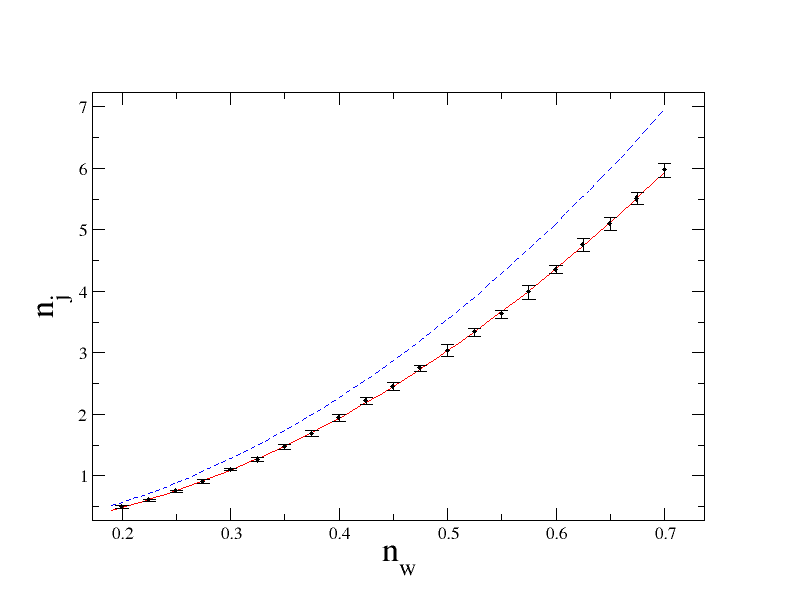
\includegraphics[width=0.49 \columnwidth]{Images/Chapter2/junctionDensity_wireDensity.png}
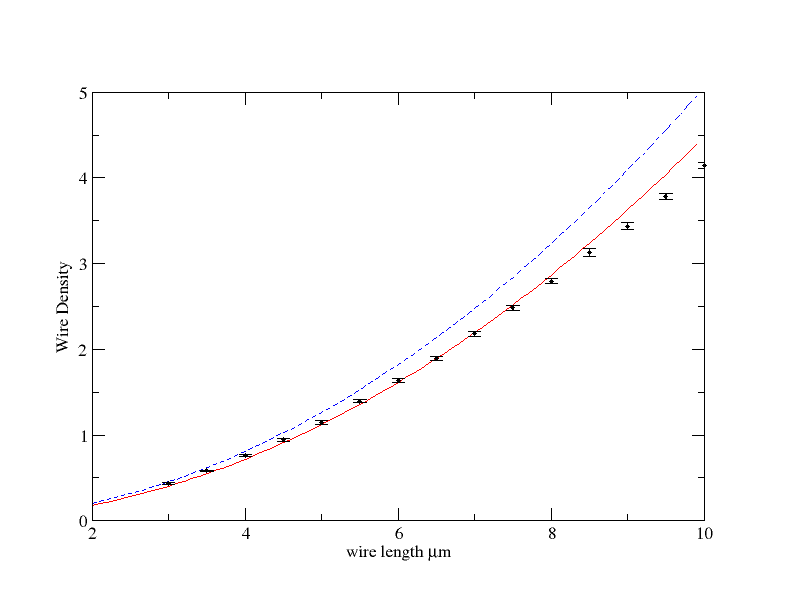
\includegraphics[width=0.49 \columnwidth]{Images/Chapter2/junctionDensity_wirelength.png}
\caption{\fontsize{10pt}{9pt}\selectfont \textit{(a) Data points are average junction density vs Wire density obtained from Monte Carlo simulations of NWNs with various wire densities, size $40 \times 40 \mu m $, and wire lengths of $6.7 \mu m^2$. Note that ten simulations were performed per wire density and the resulting 95\% confidence interval is also shown. The Blue dashed line corresponds to the analytical expression with $\omega \approx 0.316$ as derived by Heitz et al. The red curve corresponds to Equation \ref{eq:nj_nw_eqn} with $\omega = 0.27$ and agrres much closer to the Monte Carlo simulations. (b) Data points correspond to junction density vs wire lengths obtained from Monte Carlo simulations of NWNs of fixed density 0.4 Nws/$\mu m^2$ and NWN size $40 \times 40\mu m^2$. The Blue dashed again corresponds to equation \ref{eq:nj_nw_eqn} with $\omega \approx 3.16$ which overestimates the junction density at all points. The red curve corresponds to $\alpha = 0.27$ and agrees closely with the Monte Carlo results. }}
\label{fig:alpha_fit}
\end{figure}

\section{Quantum of Conductance}
The quantum of conductance appears in quantum point contacts. These are thin, short wires where there is a unity probability of electron transport across it. Consider two electron reservoirs separated by such a contact and that one electron is transported across the quantum point contact. The current is expressed as $I = \frac{e}{\Delta t}$ and voltage difference given as $\Delta V = \frac{\Delta E}{e}$ where e is the charge of an electron, $\Delta t$ is the time for the electron to be transported across the channel, $\Delta E$ is the electrochemical potential energy difference between the two reservoirs. The conductance of the channel is thus.
\begin{equation}
G_0 = \frac{I}{\Delta V} = \frac{e^2}{\Delta t \Delta E}
\end{equation}
Now the transport time and change in energy follow the uncertainty principle, $\Delta t \Delta E \leq h$ where h is Planck's constant. Therefore the $G_0 \leq \frac{e^2}{h}$. Now due to spin degeneracy the channel can allow two electrons to cross at a time. Therefore the quantum of conductance is taken as 
\begin{equation}
G_0 = \frac{2 e^2}{h}
\end{equation}

A 1 dimensional wire connects two reservoirs of electrons at potential energy $u_1$ and $u_2$. The density of states of electrons is given by 
\begin{equation}
\frac{d \rho}{d \epsilon} = \frac{2 }{h v}
\end{equation}
where $h$ is Planck's constant and $v$ is the electrons group velocity. The 2 is due to the spin degeneracy. The voltage difference between the reservoirs is $V = \frac{-(u_1 - u_2)}{e}$ where $e$ is the charge of an electron. The current flowing between the reservoirs is $I = -ev(u_1-u_2) \frac{d \rho}{d\epsilon}$. The quantum of conductance is thus
\begin{equation}
G_0 = \frac{I}{V}=\frac{2 e^2}{h}
\end{equation}
\todo{derivation of 1D dos.}
\end{comment}

\section{Chapter Summary}
\label{sec: Conclusion}
In this chapter, the necessary background theory and mathematical formalisms to understand current flow through a nanowire network were introduced, and will be referred to throughout this thesis. In section \ref{sec: Network Theory}, some fundamental aspects of network theory was introduced. Network theory was applied to an electrical network and shown to follow Kirchhoff's circuit laws. It was shown that the electrical properties of a network can be calculated by solving a system of linear equations containing the connectivity profile and resistances of the network. In section \ref{sec: Green's Function}, an analytical method to calculate resistances in an ordered infinite lattice developed by Cserti\cite{cserti2000} was presented. An approximation to the lattice Green's function solution to resistances on a square lattice was presented and shown to be very accurate, particularly at large distances. An effective medium theory for ordered resistive lattices was presented in section \ref{sec: EMT intro}. An effective medium for a two dimensional square lattice with a bi-modal resistance distribution was derived as an example. A brief introduction to percolation theory was given in section \ref{sec: Critical Density}. In particular, the critical wire density for a conductive stick system in two dimensions was presented, a density which is the lower bound to ensure an electrically conductive network between two opposite electrodes. Finally a functional form for the junction density was presented in section \ref{sec: Junction Density}, relating the junction density with wire density and wire length. 

The methods and general theory layed out in this chapter play a pivotal role in examining current flow in nanowire networks. The Kirchhoff method to calculate network resistivity is used throughout this thesis, being crucial to results presented in every chapter. The Green's function technique offers an insight into how current flows through an ordered medium which can act as a template to current-flow in a disordered one. This will be the foundation to a novel extended effective medium developed for nanowire networks which will be discussed further in chapter 4. The critical wire density determined by percolation theory is of vital importance in understanding limitations of nanowire networks with regards to sparsity and is used as a lower bound in simulations throughout the thesis. Similarly the expression for junction density in equation \ref{eq:nj_nw_eqn} and in turn the connectivity of a network is of fundamental importance for understanding the properties of networks and is used throughout the thesis. 
%\bibliographystyle{ieeetr}  %%for ordered citations
%\bibliography{bibliography}

 \chapter{Computational Models for Disordered nanowire networks}
%The aim of this chapter is to introduce the computational framework to numerically calculate the sheet resistance of a nanowire network where inner wire resistance is both included and excluded. A method to digitise SEM images of nanowire networks is presented allowing for simulations on a near identical network connectivity with physical networks whose resistance has been experimentally measured. The digitised network geometry and the inclusion of nanowire resistance allows us to estimate the inter-wire junction resistance and it is shown to agree closely with experimental measurements. A method to determine the ultimate conductivity of a nanowire network, i.e. where inter-wire junctions are perfect conductors, is presented and applied to several experimental samples. Aspects of theis work have been published in ...
%\newpage
%\section{Chapter Motivation}
The conductance of a nanowire network depends on a multitude of underlying parameters: the length and diameter distributions of nanowires\cite{hecht2006,bergin2012,sorel2012,hicks2009,pike1974}, inter-wire junction resistances\cite{mutiso2013}, resistance of nanowire segments{\cite{zezelj2012}, wire density\cite{balberg1983}}, connectivity profile, and device dimensions\cite{fairfield2014} to name but a few. All of these parameters and physical features will impact the conductance of a NWN. A common method of numerically solving this complex transport problem\cite{kirkpatrick1973} is to map the NWN onto a node-voltage graphical representation where each nanowire is a node in the graph and is connected to its nearest neighbours by a resistor corresponding to the inter-wire junction. Kirchhoff's circuit laws and Ohm's law are applied to the node-voltage graph to calculate the conductance of the system as outlined in chapter 2\cite{graph_book}. An implicit assumption is being made in this approach: the junction resistance is much higher than the nanowire inner resistance and so dominate the electrical properties of the network. This approach shall be referred to as the Junction Dominated Assumption (JDA) henceforth. 
%With such a large parameter space determining a relationship between the conductance of a NWN and the underlying parameters is difficult, requiring fitting of empirical functions to the results of large scale Monte Carlo simulations.

Monte Carlo simulations of conductive stick networks show that their electrical properties are highly sensitive to the ratio $R_{in}/R_{j}$, where $R_j$ is the resistance of a junction and $R_{in}$ is the inner resistance of a wire segment\cite{li2009,hicks2009,zezelj2012}. The JDA model has successfully calculated the resistive properties of carbon nanotube networks, as the nanotube resistance is negligible compared with the resistance of a nanotube junction\cite{nirmalraj2009,hecht2006}. Metallic nanowire junctions however have been shown to have relatively low junction resistances\cite{bellew2015} and, as a result, the nanowires themselves have a sizable impact on the network conductivity. With the demand for increasing NWN conductivity for optoelectric device applications\cite{bellet2017,gong2017,langley2013}, $R_j$ is continuously being minimised by effective annealing techniques\cite{madaria2010,hwang2014,liangbing2010,nirmalraj2012} and so the JDA is not appropriate for these systems. In this chapter, we introduce a model that includes both nanowire resistances ($R_{in}$ and $R_j$), the Multi-Nodal Representation (MNR), and show how both MNR and JDA models depend differently on the underlying parameters mentioned at the start of the chapter.

A fundamental issue with nanowire network simulations is the inherent spatial randomness of wire positions and their impact on network connectivity. Experimental measurements can only be related to the average results of simulations with matching underlying parameters in order to obtain meaningful results\cite{mutiso2013}. To directly compare computational simulation with experimental measurements, we developed a method to digitally capture the positions and orientations of nanowires from Scanning Electron Microscope (SEM) images of NWNs. The goal of this chapter is to compare MNR and JDA simulations using both configurational averaging and digitised networks from experimental samples to understand the effect of nanowire resistance on certain network properties.

The layout of this chapter is as follows. In section \ref{sec:Graphical Representations of NWNs}, the JDA and MNR models are presented and the computational simulations are outlined. In section \ref{Sec: Resistive properties}, MNR and JDA approaches are applied to simulations of NWNs and the dependence of sheet resistance on a selection of nanowire properties are explored, highlighting the impact of inner-wire resistance on these relationships. In section \ref{sec:image_proc}, an original technique that digitises images of experimental NWNs is introduced to which the JDA and MNR are applied. The digitised networks can be used to approximate the junction resistance of the samples and these results were compared with a distribution of junction resistances that were measured experimentally\cite{bellew2015}. The ultimate conductivity of a NWN, which can be obtained when junctions are annealed to their optimum capacities, is then calculated for each of the experimental samples. A novel way of quantifying the potential for network conductance improvement is introduced in section \ref{sec:image_proc} and its dependence on several network parameters is presented\cite{rocha2015}. In section \ref{Sec: Dispersion}, the effect of including dispersion in the junction resistances is examined for MNR and JDA mappings. A short chapter summary is presented in section \ref{sec:Conclusion}.
%==================================================
\section{Graphical Representations of Nanowire Networks}
\label{sec:Graphical Representations of NWNs}

To calculate the resistive properties of a NWN, the nanowire mesh must be mapped into a mathematical graph that captures the connectivity information of the network to which node-voltage points are assigned. In this way, Kirchhoff's system of linear equations introduced in chapter 2 can be used. In the JDA mapping, each wire is represented by a circuit node at a common voltage connected to other wires by junction resistors (edges of the graph). A NWN with $N_w$ wires will result in a resistive graph with $N_w$ nodes. An off-diagonal element in the Kirchhoff matrix ($K^{jda}_{ij}$) is the conductance of the inter-wire junction between wires $i$ and $j$. Figure \ref{fig: mnr_jda_sketch}(a) is a sketch of a simple NWN (top) with its JDA graphical representation (bottom). There are three nodes in this graphical representation, one for each nanowire, and two inter-wire junctions with resistance $R_j$. Note that there is no junction between wires $W_1$ and $W_2$, thus there is no resistor for this connection in the graph representation. The locations of the nanowires are irrelevant in the JDA; only the connectivity profile of the network and $R_j$ determine its electrical properties. As this mapping only acts on the inter-wire connectivity, the inner-wire resistances of the nanowire segments are entirely omitted from this model.

\fig{1.0}
{Images/Chapter3/mnr_jda_sketch_lowQ.png}
{\textbf{Schematic:} Mapping a nanowire network with JDA and MNR models.}
{ (a) A sketch of a simple NWN with three wires labeled $W_i$, $i = 1,2,3$ and two inter-wire junctions, one between wires $W_1$ and $W_2$ and another between wires $W_1$ and $W_3$\cite{rocha2015}. Underneath the sketch is a circuit representation of the NWN; there are three nodes corresponding to the three wires and two inter-wire junction resistors represented by black resistors with resistances $R_j$. (b) An expanded view of the three wires sketched in panel (a). The four connection nodes, two for each inter-wire junction, are shown as the red dots labeled $C_i, ~ i=1,2,3,4$. Underneath the sketch is an MNR circuit representation of the NWN. Connection nodes associated with the same junction are connected by a junction resistor $R_j$ and shown in black. The connection nodes that are adjacent on $W_3$, $C_2$ and $C_4$, are connected by a nanowire segment resistor $R_{in}$ illustrated by the yellow resistor.}
{fig: mnr_jda_sketch}

% MNR
While the JDA is suitable for materials with sufficiently large junction resistances, the nanowire resistance cannot be omitted for materials where it is comparable with that of the junctions. In order to include the inner wire resistances, a new voltage-node mapping is needed. Consider a wire that has $b$ intersections with other wires thus partitioning it into $b+1$ wire sections each with a classical resistance given by 
\begin{equation}
R_{in} = \frac{\rho \ell_\textit{i}}{A_c}
\end{equation}
where $\rho$ is the wire resistivity, $\ell_\textit{i}$ is the length of wire section $\textit{i}$, and $A_c = \pi (D/2)^2$ is the cross sectional area of the wire with $D$ being the diameter of the nanowire. Note that two of the sections, at either end of the nanowire, play no part in the electrical properties of the network as they are `dead-ends' for current-flow\cite{ocallaco2016}. There is the unlikely scenario where the end of the wire may touch another horizontally as opposed to forming an overlap junction, essentially forming a "T" junction. This scenario is not considered in the mapping as it accounts for a negligible number of junctions overall.
%This classical relationship holds for nanowires with relatively large diameters, where the diamters are less than or equal to the mean free path length of electrons in (approximately 40 nm in bulk Ag) there is an expected increase in electron scattering from surface roughness and grain boundaries.

The inter-wire connection points, which partition the wire segments, are the nodes in the new node-voltage mapping which we shall call Multi-Nodal Representation (MNR) henceforth. For each inter-wire junction, there are two connection nodes, one on each wire, and are connected by a junction resistor. Adjacent connection nodes on the same nanowire are joined with an inner-nanowire resistor. A sketch of a simple NWN and the corresponding MNR graph representation is presented in Figure \ref{fig: mnr_jda_sketch}(b). The total number of nodes in this scheme is $2 N_j$, where $N_j$ is the total number of junctions in the network. The nanowire resistor between the nodes $C_2$ and $C_4$ is depicted in yellow and the two junction resistors are shown in black. Note that contributions from the wires' dead-ends are not included in this representation either. Unlike the JDA model, the locations of the wires and their intersections in the network have to be considered in the MNR model as the distances between adjacent connection nodes are needed for the calculation of the nanowire resistances. 

\begin{comment}
Consider a NWN with $N_w$ wires and $N_j$ junctions. The number of current carrying wire segments $N_{cc}$ in the network are the number of wire segments $N_s$ minus two 'dead-ends' per wire.
\begin{equation}
N_{cc} = N_s - 2 N_2
\end{equation}
For every intersection on a wire, an additional wire segment occurs on it. Following this logic the number of wire segments is $N_w$ initially and for every junction in the NWN there are two wire segments created, an additional segment on each wire. Thus the total number of wire segments are 
\begin{equation}
N_s = 2N_j + N_w
\end{equation}
The number of current carrying wire segments is thus 
\begin{equation}
N_{cc} = N_s - 2 N_w = 2 N_j - N_w
\end{equation}
\end{comment}
In chapter 2, the junction density was related to the wire density in a network by $n_j = \omega L^2 n_w^2 $ meaning that the total number of junctions is $N_j = \omega L^2 N_w^2 / B$ where $L$ is the length of each wire, $B$ is the total area of the NWN and $\omega$ is a constant ($\approx 0.318$)\cite{ocallaco2016,kallmes1960,sampson2008}. The Kirchhoff matrix for the JDA model of a network is of size $N_w \times N_w$ representing a system of $N_w$ linear equations. In the MNR model, the Kirchhoff matrix is of size $2 N_j\times 2 N_j$ representing $2N_j = 2 \omega L^2 N_w^2/B$ linear equations. As the number of junctions depends on $N_w^2$, the number of equations to be solved is proportional to $N_w^2$ for the MNR model, compared with $N_w$ equations for the JDA model. Herein lies a disadvantage of the MNR model as the required computational memory and power quickly becomes too demanding for relatively large and dense networks.

In both JDA and MNR, the computational simulations conducted in random NWNs are performed as follows: a number of nanowires are randomly distributed over a predefined area. An inter-wire junction is assigned where two wires intersect; the positions and associated wires of each intersection are recorded. The MNR and JDA mappings can then be applied to the NWN from the connectivity profile and the wire positions. The Kirchhoff matrix for both can be formulated and numerically solved to calculate the sheet resistance $(R_s)$ of the network. The same network can be recreated a number of times by fixing the random number generator seed used to generate the positions and orientations of wires in the simulations. This allows the impact of particular network parameters to be assessed on a fixed geometry. Likewise, a network ensemble can be created by shuffling the wires over the device area. The two pictures are excellent tools to determine the effect of all of the underlying properties on the resulting sheet resistance of the NWN. 

The parameters of the NWN can be grouped into two main categories: the geometric and the resistive parameters. The geometric parameters are those that affect the connectivity profile of the NWN, e.g. the wire density ($n_w$) and the wire length ($L$). A change in one of these parameters will alter the connectivity profile of the NWN. For example, two networks with the same wire lengths and densities can have vastly different sheet resistances due to stochastic fluctuations in wire position and orientation. Monte Carlo simulations are then performed whereby a large number of NWNs are generated for a given wire density and wire lengths and so the effect of each parameter can be determined. Wire diameters are not used to determine the intersection of two nanowires as they are represent as widthless sticks in simulations, and so is not included as a geometrical parameter, but is considered a resistive parameter. The resistive parameters do not necessarily alter the connectivity profile of the NWN but change the magnitude of the resistors in the network. These are the junction resistance ($R_j$), and the inner-wire resistance ($R_{in}(\rho,\ell_i,D)$). The effect of these parameters are best illustrated by fixing a NWN connectivity profile and calculating the change in sheet resistance associated with changes to these parameters. The relationship between these two categories of parameters and network sheet resistance will be explored in the proceeding sections. 
% mention that Rj = 0 is a special case
%================= resistive properties =================================
\section{The Impact of Inner-wire Resistance}
\label{Sec: Resistive properties}
This section will highlight the impact of inner wire resistance on NWN sheet resistance, and is a benchmark for further simulations later in the thesis, namely in chapter 4, where the accuracy of a novel effective lattice approach for a NWN is examined. The resistive properties of nanowires are not considered to alter the connectivity of a given NWN geometry but they do impact on their resistance values. Both JDA and MNR were applied to the same network geometry in order to keep the connectivity profile fixed and allow for a direct comparison between models. Figure \ref{fig: plotNW} is a visualisation of the simulated network which is of size $20 \times 20 \mu m$, $L=7\mu m$, and $n_w = 0.4$ nanowires/$\mu m^{2}$. This network will be the benchmark geometry used to identify the dependence of the sheet resistance ($R_s$) on $R_{in}$ by changing $\rho$, $D$ and $R_j$ in this section.

\fig{0.75}
{Images/Chapter3/network.pdf}
{\textbf{Sketch:} Visualisation of a simulated nanowire network.}
{A visualisation of a simulated network to be used as a fixed geometry to determine the role of resistive parameters on network conductivity. Wires (black lines) are 7 $\mu m$ in length and the wire density is 0.4 nanowires/$\mu m^{2}$. The network has dimensions $20 \times 20 ~ \mu m$ and the electrodes are represented by the thick vertical red lines located at either sides of the network.}
{fig: plotNW}
%========================= junction ===============================
\subsection{The Relationship Between Junction and Network Resistances}
The common resistive parameter between MNR and JDA is the junction resistance. In this comparison between the models, every junction resistance was assigned the same value $R_j$, a homogeneous resistive network. The resistivity and wire diameters were fixed in the MNR to values typical of Ag/PVP core-shell nanowires, $\rho = 22.6 ~ n \Omega m$ and $D = 50 ~ nm$ \cite{rocha2015}. Figure \ref{fig: junction_res} shows the effect of increasing $R_j$ on the calculated sheet resistance for both the MNR and JDA models applied to the network geometry shown in Figure \ref{fig: plotNW}. 

\fig{1}
{Images/Chapter3/Junction_resistance.pdf}
{\textbf{Plot:} Relationship between sheet resistance and junction resistance on a fixed network geometry.}
{The effect of junction resistance on the sheet resistance of the network shown in Figure \ref{fig: plotNW}. The sheet resistance $R_s$ depends linearly on the junction resistance for both the MNR and JDA models in the case of homogeneous junction resistances. In fact, the slope of both lines ($a$) is approximately the same for both models with $a = 0.37$. The effect of the nanowire resistance in the MNR manifests with the addition of a constant $R_0$ which corresponds to $R_s^{MNR}$ when $R_j \rightarrow 0$.\cite{rocha2015}}
{fig: junction_res}

A striking feature of Figure \ref{fig: junction_res} is that the sheet resistance predicted by the MNR and JDA depends linearly on the junction resistance with the same slope as
\begin{align}
R_s^{JDA} &= a R_j  \label{eq: Rs_jda}\\
R_s^{MNR} &= a R_j + R_0 \label{eq: Rs_mnr}
\end{align}
where $a = 0.37$ for the network shown in Figure \ref{fig: plotNW}. The MNR result is offset from the JDA approach by $R_0 = 21 ~ \Omega$ and it corresponds to the contribution of the internal resistance of the nanowires. This linear dependence is for an idealised homogeneous junction resistor distribution and is shown to not hold when a level of disorder is introduced to the junction resistance distribution as discussed in section \ref{Sec: Dispersion}. The JDA functional form behaves as desired; one expects a sheet resistance of zero if every junction in the network has an idealised zero resistance. Similarly the MNR functional behaves as expected; as the junction resistance is brought to zero, the sheet resistance tends to the nanowire resistance contribution of the network $R_0$. The inclusion of the nanowire resistance increases the sheet resistance of the NWN as expected. For example, in the MNR model the $R_s \rightarrow R_0 \rightarrow 21\Omega$ for $R_j \rightarrow 0$. In order to achieve this sheet resistance in the JDA, the junction resistance required is $R_j = 21/a \approx 60 \Omega$. This difference between the required $R_j$ in both models can cause discrepancies when comparing simulations and experiments. This point is discussed further in section \ref{sec:image_proc}.

The value of the slope for both models gives an understanding of the nature of current flow through the NWN. Recently, Ainsworth\cite{ainsworth2018} et al modeled a NWN as a mesh of parallel paths between the two electrodes, all of the same length. Let there be $Y$ parallel paths of $X$ junction resistors in series, $X$ and $Y$ are characteristic parameters unique to each network. Assuming that the paths do not superimpose or interact with each other, the sheet resistance of such a network in the JDA model is,
\begin{equation}
R_s = \frac{X R_j}{Y} 
\end{equation}
Comparing this to equation \ref{eq: Rs_jda} shows that $a = \frac{X}{Y}$. Thus for $a<1$, we can argue that the current flow through the NWN is through many parallel paths $Y$, more paths than the number of junctions connected in series $X$. If $a>1$, then the current flows through few paths between electrodes. One expects that $a$ depends on the connectivity profile, where highly connected NWNs will have a much lower slope than sparse networks.

A symmetry argument can be made to explain the linear relationship between $R_s$ and $R_j$ in the JDA. If the only difference between two networks is a constant shift on every resistor value then the resistance between any nodes in the network should shift by the same amount. A mathematical proof of this can also be made by making use of the Kirchhoff Matrix formalism\cite{pozrikidis} defined in chapter 2. If every resistor in the NWN has the same value $R$, then the Kirchhoff matrix is 
\begin{equation}
{K} = \frac{1}{R} \mathcal{L} = \Gamma \mathcal{L}
\end{equation}
recalling that $\mathcal{L}$ is the Laplacian matrix defined in chapter 2 and $\Gamma = 1/R$. The Kirchhoff matrix, along with the current vector ($\vec{I}$) which defines the sourced and drained current to the network, is used to solve the potential at each node in the network. Consider the case where $R = 1$, Kirchhoff's system of linear equations are
\begin{equation}
\mathcal{L} \vec{V}^\mathcal{L} = \vec{I} 
\label{eq: temp}
\end{equation}
where $\vec{V}^\mathcal{L}$ is the solution to this equation. The resistance between the source current node ($\textit{m}$) and the drain current node ($\textit{n}$) is
\begin{equation}
R^{\mathcal{L}}_{\textit{mn}} = \frac{| \vec{V}^\mathcal{L}_\textit{m} - \vec{V}^\mathcal{L}_\textit{n}|}{i_0}
\end{equation}
where $i_0$ is the amount of current injected and drained from those nodes. Now consider the case where $R \neq 1$ and the current vector is the same as before. We now have
\begin{equation}
K\vec{V} = \frac{1}{R}\mathcal{L}\vec{V}^k = \vec{I}
\end{equation}
Using equation \ref{eq: temp}, we can equate $ \frac{1}{R}\mathcal{L}\vec{V}^K = \mathcal{L}\vec{V}^\mathcal{L}$ and so the solved voltage vectors are related by
\begin{equation}
\vec{V}^K = R \vec{V}^\mathcal{L}
\end{equation}
The resistance between the two nodes $m$ and $n$ are now
\begin{equation}
R^K_{\textit{mn}} = R \frac{| \vec{V}^\mathcal{L}_\textit{m} - \vec{V}^\mathcal{L}_\textit{n}|}{i_0}
\end{equation}
proving that the resistance between two nodes in a network of identical resistors depends linearly on their resistance assuming that current flow does not alter its course.

%======================== wire resistance =================================
\subsection{The Effect of Nanowire Resistivity and Diameter on Network Resistance}
The inner-wire resistance only plays a role in MNR, and so JDA simulations cannot be performed for these parameters. Their effect on $R_s$ was determined by applying the MNR model to the NWN pictured in Figure \ref{fig: plotNW} with $R_j =11 ~ \Omega$. Figure \ref{fig: mnr_resistivity_diameter}(a) shows the effect of changing the resistivity on the sheet resistance. $R_s$ clearly increases in a linear fashion with respect to increasing resistivity which can be attributed to the linear dependence of the resistance of wire segments on the resistivity. This increase corresponds to the shifting of $R_0$ in the linear formula for $R_s$ given in equation \ref{eq: Rs_mnr}. 
%note: Since $R_s$ depends linearly on $R_j$ it will depend linearly on any other resistance quantity one the other is kept fixed.

\fig{1.}
{Images/Chapter3/resistivity_wireDiameter.pdf}
{\textbf{Plot:} Relationship between sheet resistance and resistivity parameters on a fixed network geometry.}
{(a) Dependence of $R_s$ on the resistivity of the nanowires, specific to the network geometry shown in Figure \ref{fig: plotNW}. $R_s$ depends linearly on the resistivity of the nanowires. (b) Dependence of $R_s$ on the diameter of the nanowires $(D)$ for a fixed network geometry. This relationship follows that of the nanowire resistance on $D$ with a $D^{-2}$ dependence. In the inset, the same data is replot in green, the x axis has been recast as $D^{-2}$ highlighting the linear relationship between $R_s$ and $D$. Recall $R_s = a R_j + R_0$ and so the sheet resistance tends to a non-zero value determined by the junction resistance for vanishing nanowire resistance. The horizontal dashed line in both plots represents the sheet resistance with no nanowire resistance with $R_s = aR_j ~\approx 4.07 \Omega$ for $R_j = 11 ~ \Omega$.}
{fig: mnr_resistivity_diameter}

Figure \ref{fig: mnr_resistivity_diameter}(b) shows the effect of increasing wire diameter ($D$) on the sheet resistance of the same network. The sheet resistance decreases as a power law relationship, $R_s = c D^{-2} + aR_j$, which is expected as the nanowire resistance depends on the wire diameter as $R_{in} \propto D^{-2}$. This inverse squared relationship is clearly evident in the inset plot which is the same data with the x axis recast as $D^{-2}$. Note that a non-zero junction resistance was used in the simulations and so the sheet resistance tends to a non-zero value for vanishing resistivity and infinite wire diameter, i.e. $R_s \rightarrow a R_j$ as $R_0 \rightarrow 0$. This asymptotic sheet resistance is represented by the dashed horizontal line in both plots of Figure \ref{fig: mnr_resistivity_diameter}. If one were to consider a NWN with perfectly conductive junctions ($R_j \rightarrow 0$) then a symmetry argument similar to that used to describe the linear dependence of $R_s$ on $R_j$ can be used to describe the relationship $R_0 \propto \rho D^{-2}$. 

An important note should be raised about these symmetry arguments however; they assume that current flow does not redistribute through the network as alterations occur in the network. It is not inconceivable that in the MNR, an increase in junction or nanowire resistances could cause the current flow to alter course, thus causing a shift in the sheet resistance that does not follow the existing linear relationship.

%------------------------------ scaling properties? --------------------------
\subsection{The Impact of Wire Density on Nanowire Network Resistance}
\label{Sec: Geometric Properties}
Altering either the wire density or the wire length of a network results in a fundamental change in its connectivity profile. This change is best illustrated by the expression for the junction density derived in chapter 2, $n_j = \omega L^2 n_w^2$, as it is the junctions that determine the connectivity profile. Recall from the definitions of the JDA and MNR that the junctions are a source of resistance and determine the graphical circuit representations of the NWNs. 

The impact that geometric parameters have on the connectivity profile of the networks is also described by percolation theory\cite{pike1974}. As discussed in chapter 2, percolation theory can be used to determine quantities such as the critical wire density, $(n_w)_c$, below which a connective path does not form between two boundaries, or electrodes. This can be determined using the equation\cite{li2009} 
\begin{equation}
(n_w)_c = 5.63726 ~ L^{-2}
\label{eq: critical_wire_density}
\end{equation}
Note that equation \ref{eq: critical_wire_density} only holds for networks where all sticks are of equal length $L$. This relationship links the wire density and length at the point of criticality, and shows how the geometric parameters alter fundamental aspects of network systems. As the connectivity profile is altered in a random manner with a change in wire density, ensembles of simulations are required. The relationship between sheet resistance and the geometric parameters are then determined through averaging quantities and statistical analysis performed on the simulation ensemble.
%====================== wire density ========================

The effect of wire density on the average $<R_s>$ calculated in JDA (blue) and MNR (red) for an ensemble of NWNs is displayed in Figure \ref{fig: wireDensity}(a). Other parameters were set to values measured for Ag/PVP core shell nanowires\cite{rocha2015} that were used in the previous section: $L = 7 ~ \mu m$, $R_j = 11 ~ \Omega$, $D = 50 ~ n m$, and $\rho = 22.6 ~ n\Omega m$. Twenty simulations were performed for a given wire density in order to obtain an accurate calculation of the average $R_s$ and the associated $95\%$ confidence interval. 

From Figure \ref{fig: wireDensity}(a), the MNR model has a higher sheet resistance than for the JDA model at the same densities. This is due to the inclusion of nanowire resistances for the MNR and the junction resistances being the same in both models. There is large uncertainty in the average $<R_s>$ for simulations at lower densities ($<0.2$ nanowires/$\mu m^2$) due to being close to the critical density of $(n_w)_c = 0.11$ nanowires$/\mu m^2$ estimated by equation \ref{eq: critical_wire_density}. A sparse network is susceptible to the stochastic spatial effects of the network and the large uncertainty in the sheet resistance is a manifestation of this randomness. The general decreasing trend of the sheet resistance with increasing nanowire density is a result of additional pathways developing across the network.

\fig{1.}
{Images/Chapter3/wire_dens_final.pdf}
{\textbf{Plot:} Relationship between sheet resistance and wire density in a nanowire network.}
{(a) The effect of changing wire density $n_w$ on sheet resistance $R_s$ for networks of size $20\mu m \times 20 \mu m$ and wires of length $7 \mu m$. The wire resistivity, cross sectional area and junction resistance are those measured typical for Ag/PVP core shell nanowires. 20 random networks were simulated for each wire density in both MNR and JDA and the average sheet resistance and 95\% confidence interval for each wire density was calculated and plot. (b) Sheet resistance versus the parameter $x~= ~(n_w - (n_w)_c)$ for comparison with equation \ref{eq: percolation_scaling}. Here the two scaling regimes between $R_s$ and $n_w$ is evident for both models. Power-laws were fit to both models and are shown as dotted lines. For the MNR model the scaling exponent according to regression analysis is $\beta_{MNR} = 1.28$ and the fitted curve is shown as the black dashed line. The JDA line has an exponent $\beta_{JDA} =1.44$ and is shown as the green dashed line.}
{fig: wireDensity}

According to percolation theory\cite{pike1974}, the sheet conductance, $\Gamma_s$, of a random stick network scales as a power law with the stick density near the critical value as:
\begin{equation}
\Gamma_s \propto (n_w - (n_w)_c)^{\beta}
\label{eq: percolation_scaling}
\end{equation}
where $(n_w)_c$ is the critical wire density. This scaling law has been well documented in simulations\cite{pike1974,li2009,zezelj2012} and has been used to understand the resistive properties of carbon nanotube\cite{hu2004,hecht2006} and metallic nanowire networks\cite{nirmalraj2009,bergin2012}. Figure \ref{fig: wireDensity}(b) recasts the data from panel (a) in a log-scale plot but alters the horizontal axis to $(n_w - (n_w)_c)$ for comparison with the power law in equation \ref{eq: percolation_scaling}. Both MNR and JDA have a power law response to the increase in wire density that is easily identifiable in this plot and a linear fit is performed to on curves. The two models were found to have differing exponents in their power law fits, $\beta_{MNR}=1.28$ (black dashed line) and $\beta_{JDA}= 1.44$ (green dashed line). These differing exponents are in line with those seen in Monte Carlo simulations that have been reported in the literature\cite{li2009}. Li and Zhang showed that this scaling exponent depends on the ratio of junction resistance ($R_j$) to nanowire resistance ($R_{in}$). By fitting the Error function to Monte Carlo simulations they found the relationship between the scaling exponent and $\zeta = \log_{10}(R_j/R_{in})$ was 
\begin{equation}
\beta = \beta_0 + C~ erf(\zeta)
\end{equation}
where $\beta_0 = 1.314 \pm 0.002$ and $C = 0.108 \pm 0.003$. For the MNR model, the resistance of a nanowire of length $7~ \mu m$, $D = 50 ~ nm$, and $\rho = 22.6 ~ n \Omega m$ is approximately $ 80~ \Omega$ making $\beta_{MNR} = \beta_0 + C~erf( \log_{10}(11/80)) = 1.23$. This exponent is very close to that found with regression analysis in Figure \ref{fig: wireDensity}, $\beta_{MNR} = 1.28$, and further illustrates the importance of including nanowire resistance in calculations of the sheet resistance for networks where $R_{in}$ is non-negligible.

\begin{comment}
Note that \v{Z}e\v{z}elj and Stankovi\'c \cite{zezelj2012} have shown that exponents also have a dependence on wire density as well as the ratio of $R_j$ and $R_i$ and can vary between $1 < \beta <2$ for large wire densities but this is beyond the scope of this work.
%================ wire length ==============================
Figure \ref{fig: wireLength}(a) presents the effect of altering the wire length on the sheet resistance, while keeping wire density fixed to 0.4 nanowires/$\mu m^{2}$ in a NWN of size $20 ~ \mu m \times 20 ~ \mu m$. Other parameters are fixed to those typical for Ag/PVP nanowires given above. The results of Monte Carlo simulations for both MNR (red data points) and JDA (blue data points) models are presented. The increasing wire length causes the average sheet resistance ($<R_s>$) to decrease for both models due to the increase in network connectivity. Also the 95\% confidence interval is shown for the simulations which decreases with wire length. The MNR model consistently has a higher sheet resistance than the JDA model due to the inclusion of nanowire resistances in the simulations.

Motivated by the scaling between junction conductance and wire density, the scaling between the conductance and the parameter $L - L_c$ was plot in log-log in Figure \ref{fig: wireLength}(b). A power-law trend between sheet resistance and length is clear, and the equation $R_s\propto(L-L_c)^{-\gamma}$ for both models is fit to data. Regression analysis determined that the exponents for the power law scaling is $\gamma_{MNR} \approx 1.03$ and $\gamma_{JDA} \approx 1.45$. Similar to its effect on the scaling exponents for wire density, the inclusion of nanowire resistance drastically alters the exponents.

\fig{1}{Images/Chapter3/wire_length_final.pdf}
{\textbf{Plot:} }
{(a) The average effect of increasing wire lengths ($L$) on the sheet resistance ($R_s$) for networks with a wire density of 0.4 nanowires/$\mu m^{-2}$ and of size $20 ~ \mu m \times 20 ~ \mu m$ in both MNR and JDA models. The wire resistivity, cross sectional area and junction resistance are set to values measured for typical Ag PVP core shell nanowires with $\rho = 22.6 ~ n \Omega m$, $D = 50 ~ nm$, and $R_j = 11 ~ \Omega$ \cite{rocha2015}.The average sheet resistance of 10 nanowire networks with a given wire length is calculated for the MNR (red) and JDA (blue) and the 95\% confidence intervals are also shown. (b) The same data as that in Figure (a) recast into log-log. Here the two scaling regimes between $R_s$ and $L$ are evident for both models. Power-laws were fit to wire lengths for both models and are shown as dotted lines. For the MNR model the scaling exponent according to regression is $\gamma_{MNR} \approx 1.03$ and the fitted curve is shown as the black dashed line. The JDA line has an exponent $\gamma_{JDA} \approx 1.45$ and is shown as the green dashed line. }
{fig: wireLength}
\end{comment}
%=====================================================================================================================
\section{Digital Representation of Physical Nanowire Networks}
\label{sec:image_proc}

A key problem in comparing experimental measurements with computational simulations for nanowire networks is the need to generate an accurate numerical average. A large number of laborious simulations are required for a meaningful benchmark to compare to, and even then a physical sample could have resistances in the extreme tails of expected outcomes, particularly for sufficiently low junction density networks. To allow for a more direct comparison with physical samples, a method to digitise the geometry of an SEM image of a NWN was developed. This was achieved by opening the micrograph image of a NWN on an interactive digital canvas where the start and end positions of each wire were recorded. The wire is represented as a straight line between these points in the digital version of the NWN. A computational routine to detect intersections of the digital wires is performed to determine the positions of junctions, and to create an approximation of the connectivity profile of the physical NWN. With the positions of each wire and inter-wire junctions, a `top-down' two-dimensional representation of the NWN can be created digitally. Figure \ref{fig: digitisedNWNs}(a) shows a typical SEM image of a NWN comprising of Ag/PVP core-shell nanowires, and Figure \ref{fig: digitisedNWNs}(b) is its digitised version. The latter is in fact an approximation; from the top-down view of the SEM image, it is impossible to tell if an overlap of wires results in physical contact between them, particularly in areas of high wire density where a wire may become suspended above another wire giving the appearance of a junction but in reality there is none. This approximation works particularly well for relatively sparse networks in which there are a small number of wires piling up perpendicular to the NWN, in the $\mathcal{Z}$ direction.
%Also the digitisation method approximates every wire as straight lines; wires with significant curvature are represented with multiple kinks that underline their path.

\fig{1}
{Images/Chapter3/digitised_nwn_new.pdf}
{\textbf{Schematic:} An SEM image of a nanowire network and its digitised counterpart.}
{(a) A SEM of a physical nanowire network that is roughly $20 ~ \times 20 ~ \mu m$ in size. Nanowires can be seen against the black background with electrodes seen to the left and right sides of the network. (b) A representation of the digitised NWN depicted in (a), the network has a wire density of $0.37$ nanowires/$\mu m^2$ and $440$ junctions. Black dots mark the positions of the inter-nanowire junctions and the blue vertical lines represent the electrodes\cite{rocha2015}.}
{fig: digitisedNWNs}

The sheet resistance of the NWN in Figure \ref{fig: digitisedNWNs}(a) was measured experimentally as $R_s^{EXP} = 42.9 ~ \Omega$. By analysing the dependence of $R_s$ on $R_j$ for both MNR and JDA simulations for the digitised network, one can identify a characteristic junction resistance that will lead to the observed experimental sheet resistance. Each junction in the digitised NWN was assigned a resistance $R_j$, and wires in the MNR assigned the measured resistivity of $\rho = 22.6 ~ n \Omega m$ and diameter $D = 50 ~ nm$ for Ag/PVP nanowires. $R_s$ was calculated for both models and this process was repeated for many values of $R_j$, the results of which are plot in Figure \ref{fig: mnr_jda_exp_comp}. Also shown in Figure \ref{fig: mnr_jda_exp_comp} is the experimental sheet resistance $R_s^{EXP}$, which is represented by the horizontal dashed line. Where it intersects with the JDA sheet resistance curve ($R_s^{JDA}$) and the MNR sheet resistance curve ($R_s^{MNR}$), provides two characteristic junction resistances, $R_j^{JDA} = 96.9 ~ \Omega$ and $R_j^{MNR} = 52.9 ~ \Omega$. The difference between the characteristic junction resistances is sizable, $\Delta R_j = 44~\Omega$, illustrating the large impact the nanowire resistance has on the sheet resistance of the network.

As seen in section \ref{Sec: Resistive properties}, the two resistive curves offer much insight into the behaviour of the network. Recall that the equations for $R_s$ in terms of $R_j$ for both models are
\begin{align}
R_s^{JDA} &= a R_j\nonumber\\
R_s^{MNR} &= a R_j+ R_0
\label{eq: rs_linear}
\end{align}
where the fitting parameters are $a = 0.443$ and $R_0 = 16.2 ~ \Omega$ for the sample in Figure \ref{fig: digitisedNWNs}. Recall that the slope of the line $a$ can be used to understand how current flows through the NWN, either through a few or a large number of paths in the network. In this case $a = 0.443$ leading to the conclusion that current flows through many parallel paths, more paths than resistors in characteristic paths between electrodes. 

\fig{1}
{Images/Chapter3/4_C5_junction_res.pdf}
{\textbf{Plot:} The relationship between sheet resistance and junction resistance for a digitised network.}
{The relationship between the sheet resistance of the digitised network in Figure \ref{fig: digitisedNWNs}(a) using MNR and JDA models with increasing junction resistance ($R_j$). One finds $R_s^{MNR} = a R_j + R_0$ and $R_s^{JDA} = a R_j$ where $a = 0.443$ and $R_0 = 16.2 ~ \Omega$ from regression analysis. The horizontal line represents the sheet resistance that was experimentally measured for this sample, $42.9 ~ \Omega$. The value for $R_j$ required for the MNR and JDA to obtain a sheet resistance corresponding to that measured in experiment are identified as $R_j^{MNR} = 52.9 ~ \Omega$ and $R_j^{JDA} = 96.9 ~ \Omega$.}
{fig: mnr_jda_exp_comp}

The experimental sheet resistance for thirty electrically stressed samples were measured and their network geometry were digitised. $R_s$ versus $R_j$ curves were generated for each of the digitised network geometries in the same manner as in Figure \ref{fig: mnr_jda_exp_comp}. The linear equations for $R_s$ outlined in equation \ref{eq: rs_linear} were applied to each digitised network and their characteristic junction resistances were obtained as well as the slope $a$ and $R_0$. These values are listed for each sample in Table \ref{tab: nwn_exp} in Appendix \ref{appendix: experiment nwn}. Note that the junction resistances appear in the range $2.28\leq R^{MNR}_j \leq 152 ~ \Omega$ and $R^{JDA}_j$ in the range $42.35 \leq R^{MNR}_j \leq 185.91 ~ \Omega$, once again showing the sizable impact that the inclusion of inner-wire resistances takes on a network system. The characteristic junction resistances obtained by the MNR simulations are taken to be a more accurate estimate for the junction resistances of Ag/PVP nanowire junctions. %address this

The calculation of the characteristic junction resistance assumes that the resistances in the network are identical which is not the case in reality. The resistances of several individual Ag/PVP nanowire junctions that had been electrically stressed or thermally annealed were measured ($R_j^{EXP}$) by Bellew et al\cite{bellew2015}. The distribution of recorded resistances is shown in Figure \ref{fig: junc_res_dist} as the green dotted bars\cite{bellew2015}. The majority of junctions were found to have resistances less than $70 ~ \Omega$, however there were two junctions whose resistance were very high with values in the range $200 - 300 ~ \Omega$. These two measurements represent 6.25\% of the measured junction resistances. There is a clear spike in frequency of junction resistances in the range $10 - 20 ~ \Omega$ and the median junction resistance of $11 ~ \Omega$ occurs in this bin. Measurements of individual annealed Ag nanowire junctions by Selzer et al were reported as $25.2 \pm 1.9 ~ \Omega$\cite{selzer2016}, which is of the same order of magnitude as Bellew et al's measurements\cite{bellew2015}. Figure \ref{fig: junc_res_dist} also shows the distribution of the characteristic junction resistances from the MNR model ($R_j^{MNR}$) for the experimental samples and are represented by orange solid bars. The distribution of $R_j^{MNR}$ has a mean value of $44.9 ~\Omega$ and median value of $38.4~\Omega$, which is visibly higher than the distribution of $R_j^{EXP}$ for individual junctions. While it is higher than the measured results, it does show that the characteristic junction resistance is of the correct order of magnitude of tens of Ohms. The inclusion of nanowire resistance in the simulations results in a more accurate characteristic junction resistance; recall that the MNR resistances values are always smaller than those found with JDA. Again it should be stressed that the transport regimes of a single junction and a network of junctions are very different, and the random connectivity profile of the network will have an impact on the calculation of $R_j^{MNR}$, meaning that it should be viewed as an estimate only.
%In Figure \ref{fig: rj_a_nw_exp}(b) the slope $a$ is plot against the wire density and a clear trend is observed between the two. The decrease in $a$ as wire density increases suggests an increasing number of parallel paths between electrodes as the wire density increases as one would expect.

\begin{comment}
\fig{1}{Images/Chapter3/rj_a_exp.pdf}
{\textbf{Plot:} Rj A Exp}
{(a) The characteristic junction resistances obtained from applying MNR (red triangles) and JDA (blue dots) to 30 experimental NWN samples versus the measured wire density of said samples. No clear relationship is observed between $n_w$ and $R_j$. (b) The slope coefficient $a$ versus $n_w$ for the 30 experimental samples. }
{fig: rj_a_nw_exp}
\end{comment}

%------------------- could be added --------------------------
%NAHH The question naturally arises if the measured junction resistance distribution can reproduce the experimental sheet resistance for each sample. The a digital version of the resistance distribution shown in Figure \ref{fig: junc_res_dist}(a) was created in order to 
\fig{1}{Images/Chapter3/RjExp_distribution_both_n.pdf}
{\textbf{Plot:} Comparison of junction resistance distributions for experimental measurements and simulations.}
{The distribution of resistances measured for thirty two individual nanowire junctions are shown by the green dotted bars\cite{bellew2015}. There is a clear spike in frequency at the median resistance of $11 ~ \Omega$. The distribution of the characteristic junction resistances that were determined using MNR simulations are shown as thin solid orange bars. The average resistance is $44.9 ~\Omega$ and the median value is $38.4~\Omega$, of the same order of magnitude as that measured experimentally. The bin sizes are of size $10~ \Omega$ for both distributions.}
{fig: junc_res_dist}

The contribution of the sheet resistance due to that of the nanowire sections is captured by the quantity $R_0$, and it represents the ultimate conductivity of a network, where all of the junctions have been annealed to a perfectly conductive state. $R_0$ is listed for each of the thirty samples in Table \ref{tab: nwn_exp}, where each network has a contribution in the range of $8.9~\Omega \leq R_0 \leq 92.05~\Omega$. To quantify the potential for junction annealing in a network, a dimensionless optimisation-capacity coefficient ($\gamma$) was introduced \cite{rocha2015} that illustrates how close a network is to its ultimately conductive state,
\begin{equation}
\gamma = 1 - \frac{R_0}{R_s^{EXP}}
\end{equation}
where $\gamma$ varies between zero and one. Values of $\gamma$ close to one indicate the conductance of the network can be considerably improved by altering the values of $R_j$. When $\gamma$ is nearer to zero, the network is near its optimum conductivity, i.e. the skeletal nanowire resistance $R_0$, as all of the junctions in the network have been annealed into a perfectly conductive state. This metric provides fabricators of NWNs with an idea of the potential improvement possible in a particular network. 

Table \ref{tab: nwn_exp} in Appendix \ref{appendix: experiment nwn} contains the wire density, sheet resistance and other parameters for all thirty of the processed experimental samples. In this table, the outcomes of the digitisation techniques on the analysis of network properties are collected in one database. Looking at the optimisation-capacity coefficient in particular, no obvious correlation exists between $\gamma$ and $n_w, ~ R_0$, or $R_s^{exp}$. This suggests that each of the networks had their junctions improved in a consistent manner, i.e. annealing was not more effective for sparse networks. However a relationship between $\gamma$ and $R_j^{MNR}$ is expected as it is an estimate to the junction resistances in the network. Thus $\gamma$ increases with increasing characteristic junction resistance which is shown in Figure \ref{fig: gamma_plots}.

\fig{1}
{Images/Chapter3/gamma_RjExp.pdf}
{\textbf{Plot:} Optimisation capacity coefficient for thirty digitised NWNs.}
{The optimisation-capacity coefficient ($\gamma$) versus the MNR characteristic junction resistances ($R_j^{MNR}$) for the thirty experimental NWN samples shown in Table \ref{tab: nwn_exp} in Appendix \ref{appendix: experiment nwn}\cite{rocha2015}.}
{fig: gamma_plots}

The importance of including nanowire inner resistances in comparisons between computational simulations and experimental measurements was demonstrated in this section through the MNR model. Not only does the MNR model more accurately estimate the resistance of electrically stressed junctions, it also identifies the ultimate conductivity of a network, that which is limited by the skeletal nanowire resistance. The simulation results, unique to each experimental sample presented in this chapter, are numerical and take a great deal of sample processing to obtain. In the following chapter, an analytical approximation using methods outlined in chapter 2 for the sheet resistance in terms of the fundamental properties is presented, which provides a quick and mathematically transparent method to estimate various properties of a network.

%=========================================================================
\section{Impact of Junction Resistance Disorder}
\label{Sec: Dispersion}
Until now, the main source of randomness in a NWN has been the spatial orientations of nanowires and the resulting connectivity profile of the network. However, randomness can also arise in the parameters of the nanowires themselves such as the diameter and resistivity\cite{rocha2015}. In the previous section, we showed that the resistance of individual annealed junctions took on many different values in the distribution presented in Figure \ref{fig: junc_res_dist}, showing that junction resistances are another source of disorder. In this section, we will examine the effect that fluctuations in junction resistances can have on the macroscale NWN resistance. Junction resistance distributions are determined by a normal distribution that is confined to the range $[0,\infty)$ with a standard deviation $\sigma$ and a fixed mean value $<R_j>$ in simulations. The truncation is applied to the distribution to remove any negative resistances from simulations. The average of an ensemble of thirty sets of junction resistance distributions on an identical network geometry were used to calculate an average sheet resistance and confidence interval for each $<R_j>$ and $\sigma$ values. The network geometry used in these simulations is that of sample \#1 from Table \ref{tab: nwn_exp}, and it has an experimental sheet resistance of $R_s^{EXP} = 84.42~\Omega$. 

Figure \ref{fig: dispersion} presents the results of the simulations, the top panels are the average sheet resistances $R_s$ for a given $<R_j>$ with three different standard deviations, $\sigma = 0$ (black line), $\sigma = 20~\Omega$ (blue dashed curve), and $\sigma = 40 ~ \Omega$ (green curve). Panel (a) corresponds to the JDA mapping and panel (b) to the MNR mapping for simulations. An interesting behaviour is seen for the normal distributions with $\sigma \neq 0$, the relationship between $R_s$ and $<R_j>$ are not linear as is the case for $\sigma = 0$. For small $<R_j>$, the networks with junction resistance dispersion are much higher in resistance than the $\sigma = 0$ case, but the distributions eventually begin to converge with the linear trend of $\sigma = 0$ for high $<R_j>$ values. This is due to the removal of negative resistances from the junction distributions, i.e. the asymmetry of the distribution being relatively greater for small values of $<R_j>$. 

\fig{1}
{Images/Chapter3/dispersion.png}
{\textbf{Plot:} The effect of junction resistance dispersion on calculated sheet resistance.}
{The result of including junction resistance dispersion on the calculated sheet resistance $R_s$ for increasing mean junction resistance $<R_j>$ for the JDA model in panel (a) and the MNR model in (b). The digitised geometry of network sample \#1 from Table \ref{tab: nwn_exp} is used for each simulation reported here and $R_s^{EXP} = 84.42~\Omega$ is displayed by the red dashed line in panels (a) and (b). The junction resistances follow a normal distribution confined to the range [$0,\infty$) and two standard deviations are shown, $\sigma = 20 ~ \Omega$ (green curve) and $\sigma = 40 ~ \Omega$ (blue dashed curve). The linear relationships between $R_s$ and $<R_j$> for homogeneous resistance distribution, $\sigma = 0$, are shown in black. Only error bars for $\sigma = 40~\Omega$ are shown for ease of viewing. The relative variance between the mean value of $R_s$ for the distribution of $R_j$ and the homogeneous simulations are shown in the bottom panels, (c) corresponding to the JDA and (d) to the MNR\cite{rocha2015}.}
{fig: dispersion}

The bottom panels of Figure \ref{fig: dispersion} quantifies the disagreement of $R_s$ for the homogeneous and dispersed junction resistance distributions. The relative sheet resistance variance for the two curves representing dispersed distributions are shown for the JDA model in panel (c), and for the MNR model in panel (d). The relative variance was calculated by subtracting the curves with and without dispersion, $\Delta R_s = |R_s(\sigma) - R_s(\sigma = 0)|$, and dividing by $R_s(\sigma)$. The $\sigma = 40 ~\Omega$ simulations display a higher variance than $\sigma = 20 ~ \Omega$ but both reach similar low values for large values of $<R_j>$. The spread in junction resistances alters the value of the characteristic junction resistance $R_j^{MNR}$, the value of $<R_j>$ that gives a simulated $R_s$ matching with $R_s^{exp} = 84.42 ~ \Omega$ that was measured experimentally for this particular network geometry\cite{rocha2015}. The effect of junction resistance dispersion does not have a large impact in the value of $R_j^{JDA}$; the three simulation curves agree closely at this point in Figure \ref{fig: dispersion}(a). The dispersion does play a large role in MNR estimates of the characteristic junction resistance however. In Figure \ref{fig: dispersion}(b), the intersection of the $\sigma = 40 ~ \Omega$ curve, or $R_j^{MNR}(\sigma = 40)$,  occurs in the range of $0-10~\Omega$ compared with $R_j^{MNR}(\sigma = 0) = 27.73 ~\Omega$. This demonstrates the impact resistance variance can have on the sheet resistance of a NWN, the resistance dispersion can lead to a much lower $R_j^{MNR}$ according to the degree of this dispersion.

It should be noted that here only the junction resistance had a degree of dispersion but it has been demonstrated that Ag/PVP nanowires display a certain variation in wire diameter and resistivity also\cite{rocha2015}. As NWNs are comprised of many individual components, care must be taken to account for the variability of different properties of the ensemble of nanowires that collectively form the network. In chapter 4, an approximation for the effective medium lattice of a NWN is introduced, which can be used to quickly estimate the effect of introducing more complex resistance distributions on a NWN.

\begin{comment}
Finally the experimental sheet resistance was plot against the quantity $x = n_w-(n_w)_c$ in Figure \ref{fig: Rs_exp_scaling} in order to confirm the scaling relationship between the two that was shown in simulations in Section \ref{Sec: Geometric Properties} The critical wire density was calculated with the average wire length $L=6.7\mu m$. Alongside the data points is a power law with exponent $-1.44$, as was shown to hold for simulations of NWNs that included nanowire resistance. Admittedly there is large variance in the experimental sheet resistance but the shown power law does fit the data quite well. A large source of the disagreement may lie in the variance in wire lengths, for example the distribution of wire lengths for a typical sample is shown in the Appendix section \ref{sec: appendix_wire_length} which would in turn effect the critical wire density that should be used. Due to the random nature of wire placement and junction resistances one expects the variance in sheet resistance to be higher at lower wire densities which is indeed the case in Figure \ref{fig: Rs_exp_scaling}. \footnote{May not include this last paragraph and plot, same as the scaling section previously. See footnote 1}

\fig{1}
{Images/Chapter3/nw_Rs.pdf}
{\textbf{Plot:} Critical}
{The experimental sheet resistance $R_s$ versus $n_w - (n_w)_c$. The critical wire density was calculated as 0.11 NW/$\mu m^2$ corresponding to wires of length $6.7 \mu m$. The red dashed line represents the power law  $R_s \propto (n_w - (n_w)_c)^{-1.44}$, the same scaling that was identified in simulations of random NWNs in Figure \ref{fig: wireDensity}(b).}
{fig: Rs_exp_scaling}
\end{comment}
\section{Chapter Summary}
\label{sec:Conclusion}
The importance of including the contribution of nanowire inner resistance when calculating that of a nanowire network was highlighted in this chapter. Not only did the inclusion of inner-wire resistances change the dependence of the network on certain fundamental network properties, it determined the ultimate conductivity of a network with perfectly annealed junctions. 

The electrical properties of NWNs can be calculated by mapping the NWN onto a node-voltage lattice, the electrical properties of which can be numerically solved using Ohm's and Kirchhoff's laws, as discussed in chapter 2. Two node-voltage mappings were introduced in section \ref{sec:Graphical Representations of NWNs}, the Junction Dominated Approach (JDA) and the Multi-Nodal Representation (MNR). The JDA model assumes that the electrical properties of the network are dominated by the junction resistances and so the nanowire resistances are ignored while the MNR model includes them. 

The dependence of the sheet resistance ($R_s$) on various network parameters were studied in section \ref{Sec: Resistive properties} and there the effect of including the inner-wire resistance on those dependencies were examined. In the MNR model, wire resistivity ($\rho$) and wire diameter ($D$) were shown to relate to the sheet resistance as $R_s = C \rho D^{-2} + a R_j$ where $C$ is a constant and $a R_j$ is the contribution of the junction resistances for a homogeneous distribution of $R_j$'s. A linear relationship between sheet resistance and junction resistance ($R_j$) was shown to hold mathematically and in simulations for JDA models of NWNs such that $R_s^{JDA} = a R_j$. The same linear relationship was shown in simulations of MNR models of NWNs plus a contribution from the nanowire resistance, $R_s^{MNR}=a R_j + R_0$. Since networks with the same wire density can have different connectivity profiles, the need for spatial configurational averaging arose. A large number of simulations altering the wire density were performed and the corresponding average sheet resistances were plot for MNR and JDA. A power law relationship between sheet resistance and wire density was observed, as one would expect from percolation theory. The inclusion of nanowire resistance was shown to alter the value of the exponent in the percolative power laws.

A method to capture the geometrical layout of a physical NWN sample from an SEM image was presented in section \ref{sec:image_proc} which allows for simulations on geometries similar to the experimental samples. Thirty samples whose sheet resistance had been measured were digitised and they were used to understand the nature of current flow and junction resistances in real NWN samples. Linear expressions relating the sheet and junction resistances were found for each sample using MNR and JDA simulations. These were used to determine a characteristic junction resistance, the value at which the simulated $R_s$ matches the experimental $R_s^{EXP}$. The characteristic junction resistance was found to be lower for MNR model than the JDA model which can be explained with the sizable impact of nanowire inner resistances on networks. The distribution of MNR characteristic junction resistances was compared with a distribution of single Ag/PVP junction resistances measured experimentally by Bellew et al \cite{bellew2015}. The simulated characteristic resistances overestimated the measured junction resistances, but were found to be of the same order of magnitude of tens of Ohms. Characteristic junction resistances calculated with the MNR model were more accurate than those from the JDA model further highlighting the need for nanowire resistances to describe metallic NWNs.

The ultimate conductivity of a network was shown to be limited by the contribution of the nanowire resistances in section \ref{sec:image_proc}. A measure of how much potential for conductivity improvement was introduced with the optimisation-capacity coefficient ($\gamma$). This quantity was calculated for all thirty experimental samples. $\gamma$ was shown to depend on the characteristic junction resistance, where NWNs with higher sheet resistances had higher values of $\gamma$, meaning that there was much room for improvement to their conduction characteristics if somehow $R_j$ could be decreased.

The impact junction resistance dispersion can have on the sheet resistance of a NWN was demonstrated in section \ref{Sec: Dispersion}. Here it was shown that dispersion can break the linear relationship between $R_s$ and $R_j$ demonstrated in section \ref{Sec: Resistive properties}. A digitised network geometry was used to show that the non-linear relationship between $R_s$ and $<R_j>$ for dispersed junction distributions can shift the characteristic junction resistance to lower values compared to estimates obtained with homogeneous simulations. 
%Finally the measured sheet resistance was shown to scale with the wire density as expected from percolation theory. The exact power law found from simulations of computationally generated random NWNs was shown to describe that of the experimental samples well, however samples with low wire densities had sizable variance in the measured sheet resistance.

%\bibliographystyle{ieeetr} %%for ordered citations
%\bibliography{bibliography}

%\section{notes}
%If needed could add junction resistance distribution for charachteristic junction resistance, could do simulations using measured junction distribution with outliers until Rs match.

\begin{comment}

\section{Appendix}
\subsection{Wire Length Distribution}
\label{sec: appendix_wire_length}
A complete wire length distribution can easily be determined through the digitised networks. Fig. \ref{fig: wireLength_Dist} b) shows the wire length distribution associated with the digitised network displayed in Fig. \ref{fig: wireLength_Dist} a). A large amount of short nanowires are present in network and wire length peaks at $\approx 7 \mu m$. There is a low frequency of wires with a length greater than $7 \mu m$, the longest wire at $22.7\mu m$. 

\begin{figure}[h!]
\centering
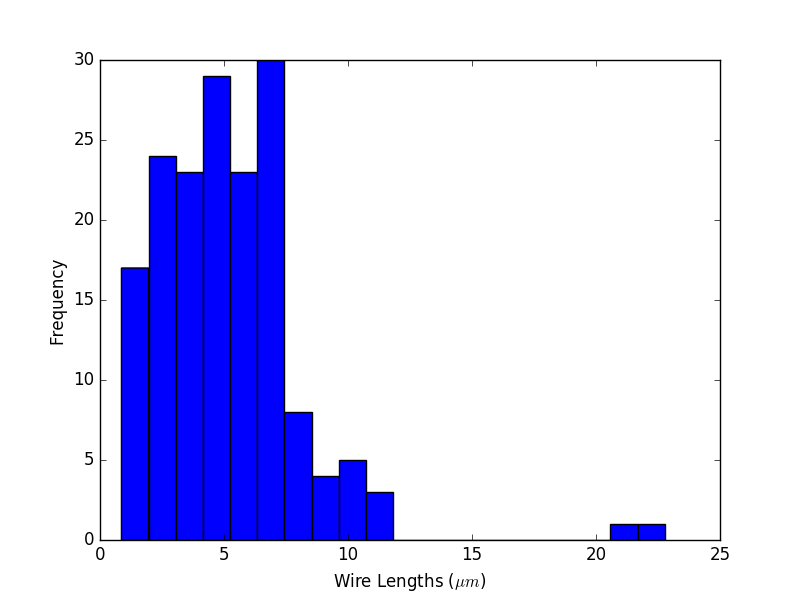
\includegraphics[width=0.7 \columnwidth]{Images/Chapter3/wireLengthDist.png}
\caption{\fontsize{12pt}{11pt}\selectfont Frequency distribution of the wire lengths obtained the digitised NWN shown in Fig. \ref{fig: digitisedNWNs} b). There are a large number of short NWNs with a peak in frequency at around $7 \mu m$ and a quick drop off in wire lengths after this. The mean wire length for this sample is $5.16 \mu m$ and median wire length $4.89 \mu m$.}%
\label{fig: wireLength_Dist}
\end{figure}
\end{comment}


 % MNR JDA
 \chapter{Effective Medium Theory for Nanowire Networks}

A difficulty with NWN adaptability for use in devices at an industrial scale is their random nature. The random connectivity profile, and varying junction resistances and wire resistivity all conspire to make the fabrication of a NWN with a desired sheet resistance difficult. Two NWNs comprised of identical wires and of similar wire densities can have wildly different electrical properties due to the inherent network disorder, frustrating reproducibility in experiments. In simulations, this large variance is caused by two main types of disorder: the randomness with which wires are spatially distributed\cite{ kallmes1960, sampson2008} and the inherent fluctuations on the characteristics of the individual wires. This calls for averaging strategies that reduce the impact of these fluctuations in any calculations, requiring a large amount of computational resources to determine the average sheet resistance for fixed nanowire properties, as was seen in chapter 3. With that in mind, a novel method that processes Scanning Electron Microscope (SEM) images of NWNs and captures the precise locations of all wires of a given sample was presented in chapter 3. An example of an SEM image is presented in Figure \ref{fig: nwn_mapping_sketch}(a), and its digitised form is shown in Figure \ref{fig: nwn_mapping_sketch}(b). This establishes a benchmark connectivity the NWN possesses and removes the need for averaging over the wire locations, consequently reducing the fluctuations induced by spatial disorder. A matching connectivity profile for experiment and simulations allows for an extraordinary level of simplification in simulation and experiment comparisons. A further simplification can be made through a theoretical description of the electrical properties of a network giving a method to quickly estimate the characteristics of a real NWN sample. In this chapter, such an expression is succesfully derived for a NWN by developing a mapping to an effective medium lattice whose sheet resistance can be calculated with a closed-form expression\cite{ocallaco2016}.

Contemporary theoretical descriptions of real-world NWNs in which their physical characteristics are accounted for is typically done by means of robust Monte-Carlo procedures used to determine universal behaviours of simplified computer-generated NWNs \cite{pike1974,li2009,zezelj2012,ashkan2007,khanarian2013,ainsworth2018}. However, a method to obtain a closed-form analytical expression for the conductance of infinite ordered homogeneous networks is known\cite{cserti2000}, and was discussed in chapter 2. Whether this method can be of use to describe heavily disordered structures, even though they are far from ordered, is the strategy adopted in this chapter. By mapping the disordered structures onto a corresponding effective square lattice that was discussed in chapter 2 for instance, we can obtain the sheet resistance of a NWN with an arbitrarily large density of wires. This mapping is visualised in Figure \ref{fig: nwn_mapping_sketch} where the resistive network graph in panel (c) will be discussed as an effective square lattice shown in panel (d). Further manipulation of these representations enables us to describe the conductivity of these films under real experimental conditions. In fact, we show that dense networks composed of nanowires of non-uniform lengths and diameters contacted by finite-sized electrodes can be described by this approach\cite{ocallaco2016}.

\fig{0.8}
{Images/Chapter4/nwn_network_sketch_hq.pdf}
{\textbf{Sketch:} The steps of mapping a NWN image onto an effective lattice.}
{(a) SEM micrograph image of a Ag/PVP NWN with hundreds of wires randomly distributed on top of an insulating substrate. Two electrodes on both sides of the sample, shown as vertical gray bars, are connected by numerous paths formed by the wires. (b) After the image is processed, the digitized version of the image records each wire location and provides full information about the intersection points of each wire\cite{rocha2015}. (c) A mathematical graph of a digitised network such as that in panel (b) showing voltage nodes as points and connecting resistors as edges. (d) The simplified graph of a square lattice representing a regular ordered network\cite{ocallaco2016}. }
{fig: nwn_mapping_sketch}

The sequence of this chapter is as follows. In section \ref{Sec: Inter node}, the equivalent resistance between two nanowire junctions in a random NWN is shown to behave in a similar manner to the equivalent inter-nodal resistance in an infinite square lattice that was discussed in chapter 2, suggesting that a mapping between the two systems can be established. An Effective Medium Theory (EMT) is introduced for regular lattices, and is then used to determine this mapping between a square lattice and a random NWN in terms of the underlying properties of the constituent nanowires in section \ref{Sec: NWN EMT}. Following this, the resistance for a multi-input/output electrode system is discussed, in particular for a system where the electrodes span opposite sides of a finite square lattice in section \ref{Sec: Inter Electrode}. By combining the effective lattice mapping for a NWN with the multi-electrode resistance expression, a closed-form expression is successfully derived for the resistive properties of a NWN based on all of the relevant nanowire properties. This expression is then used to determine various parameters and properties of NWNs that were discussed in chapter 3; this is presented in section \ref{Sec: EMT Application}. Finally a chapter summary is presented in section \ref{Sec: EMTGF Conclusion}. 

%==============================================
\section{Inter-nodal Resistance in a Nanowire Network}
\label{Sec: Inter node}
In chapter 2, an expression for the equivalent resistance between two nodes in an infinite resistor lattice was derived using the Green's function method\cite{cserti2000}. An approximation to the Green's function was derived and shown to be highly accurate for increasing separation between nodes in the lattice. Where two nodes are separated by the lattice vector $\vec{r}$, the approximation for the inter-nodal resistance is\cite{cserti2000} 
\begin{equation}
R_{eq}(\vec{r}) \approx \frac{R}{\pi} \left( \ln(|\vec{r}|) + \gamma + \frac{\ln(8)}{2} \right) 
\label{eq: Rnn_approx}
\end{equation}
where $R$ is the resistance of each edge in the lattice and $\gamma = 0.5772...$ is the Euler-Mascheroni constant. Equation \ref{eq: Rnn_approx} was shown to match the equivalent resistance calculated numerically for a finite square resistive lattice using Kirchhoff's and Ohm's laws in chapter 2. With an understanding of the electrical properties of inter-nodal currents in ordered resistive networks, the question arises if current flow in NWNs behaves in a similar manner. In Figure \ref{fig:inter_node_nwn_sketch}, a sketch of several nanowires is shown with two electrode nodes represented by red dots. For an accurate comparison with a resistive lattice, the distance metric used will be the nodal distance, or the number of resistors in the shortest path between two electrodes. Figure \ref{fig:inter_node_nwn_sketch} is a sketch of a NWN where the shortest nodal path between the two electrodes is depicted with blue arrows. The path contains three wire segments and one inter-wire junction making the nodal separation equal to four.  

\fig{0.75}
{Images/Chapter4/inter_node_sketch_proper.pdf}
{\textbf{Sketch:} Visualisation of nodal separation.}
{A sketch of a NWN with nanowires represented as grey cylinders, and the source and drain electrodes as red circles. The shortest path between electrodes is traced with the blue arrows through a single nanowire junction represented as a black circle and three wire segments, making the nodal separation between the electrodes equals four.}
{fig:inter_node_nwn_sketch}

A large NWN with no bounding electrodes was simulated to calculate the relationship between $R_{eq}$ and the nodal separation for an ensemble of pairs of nodes, using the MNR node-voltage mapping to include inner-wire resistances. The simulated nanowires were all of length $L =7 ~ \mu m$, junction resistance $R_j = 11 ~ \Omega$, wire resistivity $\rho = 22.6 ~ n \Omega m$, and wire diameter $D = 60 ~ nm$. The average inter-nodal resistance for a given nodal separation is shown in Figure \ref{fig:free_inner_res}. Immediately one identifies that the resistance between nearest neighbours is relatively large and uncertain. This large variance is due to the nearest neighbour being either a junction or an inner-wire segment which itself has a large variance as it depends on the length of that wire segment. The uncertainty decreases for increasing nodal-separation due to the fluctuations of inner-wire resistance values and junction resistances being averaged over. At larger separations, the uncertainty grows once again. This is likely due to finite sized effects as one or both of the nodes begin to reach the edge of the network. There is an unmistakable trend between $R_{eq}$ and the node separation which appears log-like but the large error bars in the data points might obscure this. The green line in Figure \ref{fig:free_inner_res} corresponds to a fit of equation \ref{eq: Rnn_approx}, where the effective resistance was the fitting parameter and found to be $R = 6.09 ~ \Omega$. This suggests that the inter-nodal resistance in a random NWN can be approximated using an expression derived for a regular square lattice, requiring only an appropriate effective resistance that represents both the wire segment and junction resistances. A method to calculate an effective resistance is outlined in the following section. 

\fig{1}
{Images/Chapter4/free_inner.pdf}
{\textbf{Plot:} Equivalent resistance between nodes in a NWN.}
{ The inter-nodal resistance ($R_{eq}$) for a given nodal separation in a random NWN. The resistance between nodes is calculated using the MNR model which was described in chapter 3, thus including the effect of inner-wire resistance. The red points correspond to the average $R_{eq}$ for a given node separation and the error bars are 95\% confidence intervals. The green line is the fitting of equation \ref{eq: Rnn_approx} where $R = 6.09 ~ \Omega$ is the fitting parameter.}
{fig:free_inner_res}
%=========================================================================
\section{Effective Medium Theory of a Nanowire Network}
\label{Sec: NWN EMT}
In chapter 2, the Effective Medium Theory (EMT) for conduction in resistive lattices\cite{kirkpatrick1973} was introduced where a network whose conductor values $g$ follow some distribution $f(g)$ and can be mapped onto a homogeneous network that has the same average properties. The effective resistance is calculated such that the average resistive properties of the homogeneous and inhomogeneous networks are the same. An effective medium theory requires an understanding of the resistor distribution $f(g)$, both the resistance values and relative proportions of each. With several assumptions, patterns can be identified in the types of resistors that make up a NWN. In this section, the different types of resistors in a NWN are established and analytical expressions to calculate their relative populations are derived. 

In the MNR voltage mapping each node has three edges connected to it, one junction resistor and, either two inner-wire segments or a single wire segment and a `dead-end'\cite{ocallaco2016}. Dead-ends occur at either end of a nanowire (two per nanowire), and are represented by an infinite resistance connection $R_d \rightarrow \infty$. Mathematically, the number of dead-ends in a network is $N_d = 2 N_w$, $N_w$ being the total number of nanowires. The number of junction resistors is $N_j$ and each of their values will follow some junction resistance distribution $\sigma_j(R_j)$. Finally there are current carrying inner-wire segments whose relative percentages can be derived with the following logic: consider a network with no inter-wire junctions; the number of wire segments is clearly the number of wires in the network. For every inter-wire junction that is added to the network, two wire segments are formed (one on each wire). Thus the total number of wire segments $N_s$ is
\begin{equation}
N_s = N_w + 2 N_j
\end{equation}
This expression for the number of segments includes dead-ends, and so the number of current-carrying wire segments is 
\begin{equation}
N_{cc} = N_s - N_d = 2 N_j - N_w
\end{equation}
Figure \ref{fig:nwn_emt_sketch} presents a sketch of a simple NWN that identifies the different types of resistors. In this network, $N_w = 5$ and $N_j = 5$, and so there are $N_d = 10$ dead-ends which are coloured in blue and there are $N_{cc} = 5$ current carrying segments coloured in red.

\begin{comment}
\fig{1}
{Images/Chapter4/simple_nwn_component_final.pdf}
{\textbf{Sketch:} Types of resistors in a NWN.}
{(a) A sketch of a NWN and (b) the different types of resistors highlighted in the network. In this network, there are five wires ($N_w = 5$) and the five junctions ($N_j = 5$) depicted by black circles. There are ten dead-ends ($N_d  = 10$) and these are depicted by blue segments. There are five current-carrying segments, $N_{cc} = 2 N_j - N_w$, shown in red. In total there are $N_t = N_j+ N_d + N_{cc} = 20$ resistors in this network.}
{fig:nwn_emt_sketch}
\end{comment}
\fig{0.75}
{Images/Chapter4/simple_nwn_component.pdf}
{\textbf{Sketch:} Types of resistors in a NWN.}
{A sketch of the different types of resistors in a NWN, where each is highlighted. In this network, there are five wires ($N_w = 5$) and the five junctions ($N_j = 5$) depicted by black circles. There are ten dead-ends ($N_d  = 10$) and these are depicted by blue segments. There are five current-carrying segments, $N_{cc} = 2 N_j - N_w$, shown in red. In total there are $N_t = N_j+ N_d + N_{cc} = 20$ resistors in this network.}
{fig:nwn_emt_sketch}


The total number of conductors $N_t$ is the sum of inter-wire junctions $N_j$ and wire segments including dead-ends as
\begin{equation}
N_t = N_j + N_{cc} + N_d = 3 N_j+N_w
\end{equation}
The relative percentages of each type of resistor is thus
\begin{eqnarray}
P_j &=& \frac{N_j}{3 N_j+N_w} \nonumber \\
P_{cc} &=& \frac{2 N_j - N_w}{3 N_j+N_w} \nonumber \\
P_d &=& \frac{2 N_w}{3 N_j+N_w}
\end{eqnarray}
where $P_j$ is the percentage of junction resistors, $P_{cc}$ the percentage of current carrying wire segments, and $P_d$ the percentage of dead-ends. These relative populations can be easily translated into expressions in terms of junction and wire densities by dividing both numerator and denominator by the area of the network. In chapter 2, an expression relating the junction density with the wire density of a nanowire network with wires of length $L$ was derived as\cite{kallmes1960,sampson2008,ocallaco2016} $n_j = \omega L^2 n_w^2$ where $\omega = \pi^{-1} \approx 0.318$. Following this expression the relative percentages in terms of wire densities and their lengths are given by
\begin{eqnarray}
P_j &=& \frac{ \omega L^2 n_w}{3 \omega L^2 n_w + 1} \nonumber \\
P_{cc} &=& \frac{2 \omega L^2 n_w - 1}{3 \omega L^2 n_w + 1} \nonumber \\
P_d &=& \frac{2 }{3 \omega L^2 n_w + 1}
\label{eq: resistor_percentage}
\end{eqnarray}
Equations \ref{eq: resistor_percentage} allow one to calculate the population of each type of resistor in a NWN knowing only the total number of wires and their length. This is a more desirable form for the relative percentages of populations as it does not require one to explicitly count the number of junctions in a NWN. The nanowire density and typical wire lengths are predefined parameters in typical Monte Carlo simulations and are straightforward to measure in physical NWN samples. An important note with respect to equations \ref{eq: resistor_percentage} is that they hold for networks where all wires are of length $L$ as this is a condition for the calculation of $n_j$. 

\fig{1}
{Images/Chapter4/relative_percentages.pdf}
{\textbf{Plot:} EMT relative percentages of resistors in a NWN.}
{A plot of the relative percentages of the different types of resistors in a NWN as a function of wire density for a NWN with wire lengths of $7\mu m$. The red curve is the percentage of current-carrying wire segments $P_{cc}$, the black curve is the percentage of junctions $P_j$ and the green curve is the percentage of dead ends $P_d$. The vertical purple dashed line is the percolative critical wire density $(n_w)_c$ at which a percolative path occurs in 50\% of randomly generated networks with this density\cite{li2009}.}
{fig:emt_nwn_percentages}

Figure \ref{fig:emt_nwn_percentages} presents a visualisation of these relative percentages as a function of wire density for a NWN with nanowires of length $7 ~ \mu m$. Note that as the wire density tends to infinity, the percentage of dead-ends tends to zero, while the number of junctions tends to 1/3 and the number of current-carrying segments tends to 2/3. As mentioned previously, each node in MNR has three nearest neighbours and is connected to a junction resistance and either two-current carrying wire segments or one current-carrying wire segment and a dead end. As the number of wires tends to infinite, the percentage of dead-ends drops to zero and so the percentages tend to the 1/3 junctions and 2/3 current-carrying segment percentages. On the other extreme, a critical wire density of sorts can be identified at which the percentage of current-carrying segments is zero according to the definition of $P_{cc}$ in equation \ref{eq: resistor_percentage}.
\begin{equation}
(n_w)_0 = \frac{1}{2 \omega L^2}
\end{equation}
For wire lengths of $L = 7 ~ \mu m$, this gives $(n_w)_0 \approx 0.035$ nanowires/$\mu m^2$. At this value there are only dead-ends and wire junctions which does not result in a conductive network as there are no conducting wire segments through which current can flow. $(n_w)_0$ is the minimum wire density that is considered in Figure \ref{fig:emt_nwn_percentages} as below this density $P_{cc}<0$.

The population of each type of resistor is only one of the components to the full conductance distribution $f(g)$. One also requires the distribution in conductance values of each type of resistor. Recall from chapter 2 that the effective conductance $g_m$ is calculated using the following equation\cite{kirkpatrick1973} 
\begin{equation}
\int \frac{g_m-g}{g+(z/2)g_m} f(g) ~ dg = 0
\label{eq:emt_def}
\end{equation}
where $z$ is the degree of each node in the lattice. In general, the distribution for NWNs to be used in equation \ref{eq:emt_def} is:
\begin{equation}
f(g) = P_{cc} \sigma_{cc}(g) + P_j \sigma_{j}(g) + P_d \delta(g) 
\label{eq: long_nwn_conductance_dist}
\end{equation}
where $\sigma_{cc}(g)$ is the distribution of inner-wire conductances, $\sigma_{j}(g)$ is the distribution of junction conductances, and since all dead-ends have a conductance $g=0$, its distribution is characterised by the Dirac delta function $\delta(g)$. While the populations of each type of resistor have been given in equation \ref{eq: resistor_percentage}, the distributions to be used for the junction and inner-wire resistances have not. The junction resistances in Monte Carlo simulations are usually fixed to some homogeneous value $g_j$ and so $\sigma_{j}(g) = \delta(g-g_j)$. The conductance of a current carrying inner-wire segment is given by $g_{cc} = \frac{A_c}{\rho \ell}$ where $\rho$ is the resistivity, $A_c$ the cross sectional area, and $\ell$ the length of the wire segment. The inner-wire conductance distribution will be approximated by the average length of a wire segment $\tilde{l}_s$, and is calculated by dividing the total length of all the wires by the number of wire segments in the network. 
\begin{equation}
\tilde{l}_s= \frac{L N_w}{N_s} = \frac{L N_w}{N_w + 2 N_j}
\end{equation}
where $L$ is the length of each wire. It follows then that the characteristic inner-wire conductance is $g_{cc} = A_c/\rho \tilde{l}_s$ making the conductance distribution $\sigma_{cc}(g) = \delta(g - g_{cc})$. Equation \ref{eq: long_nwn_conductance_dist} simplifies to
\begin{equation}
f(g) = P_{cc} \delta(g - g_{cc}) + P_j \delta(g - g_j) + P_d \delta(g)
\label{eq: simple_nwn_conductance_dist}
\end{equation}
This approximation of the conductance distribution in NWNs can now be used to solve for the effective conductance of an ordered square lattice. Solving equation \ref{eq:emt_def} for a square lattice (degree $z = 4$) and with the distribution given in equation \ref{eq: simple_nwn_conductance_dist} the effective conductance is given by\cite{ocallaco2016}
%\begin{align}
%g_m &= \frac{g_j (N_w - 3 N_j) - 2g_{cc} N_w}{6N_j - N_w} +\frac{1}{6N_j N_w} \Big(9g_{cc}(8g_{cc} + g_j) N_j^2 - \nonumber \\
%& - 6g_{cc} N_j N_w(8g_j+g_{cc}) +(2g_{cc}+g_j)^2N_w^2 \Big)^{\frac{1}{2}} \label{Eq:gm_nwn_original}
%\end{align} NEW
\begin{align}
g_m &= \frac{g_{cc}(N_j - 3 N_w) - g_j(N_j+N_w)}{6 N_j + N_w} + \frac{1}{6 N_j + N_w} \times \nonumber \\
&\times \Big( 12 g_{cc} g_j (N_j - N_w) (3 N_j + N_w) + (g_{cc} (N_j - 3 N_w) - g_j (N_j + N_w))^2 \Big) ^{1/2}\label{Eq:gm_nwn_original}
\end{align}
Rewriting the number of junctions in terms of the wire density using the relationship $n_j = \omega L^2 n_w^2$, the effective conductance can be written as\cite{ocallaco2016}
\begin{eqnarray}
g_m = &\frac{g_{cc}(\omega L^2 n_w -3) - g_j (1 + \omega L^2 n_w)}{2+6\omega L^2 n_w^2} +\frac{1}{2+6\omega L^2 n_w} \Big( 12 g_{cc} g_j(\omega L^2 n_w -1)(1+3\omega L^2 n_w) \nonumber +\\
&+ (3 g_{cc} +g_j +\omega(g_j-g_{cc})L^2 n_w)^2 \Big)^{1/2} 
\label{eq:gm_nwn_wiredens}
\end{eqnarray}
Recalling the definition of the characteristic inner-wire resistance, equation \ref{eq:gm_nwn_wiredens} is an expression in terms of the wire length, density, diameter, resistivity, and junction resistance which are all predefined parameters of a NWN. This means simulations are not required to calculate the parameters for the effective conductance.

Revisiting the inter-nodal resistance for a NWN shown in Figure \ref{fig:free_inner_res}, the effective resistance calculated using equation \ref{eq:gm_nwn_wiredens} and parameters matching those of the simulated network is $R_{EMT} = 6.01~\Omega$. Recall that in Figure \ref{fig:free_inner_res}, equation \ref{eq: Rnn_approx} was fit to the simulation data with the resistance $R$ as the only fitting parameter resulting in $R_{fit} = 6.09~\Omega$. Figure \ref{fig:nwn_emt_log} presents the data shown in Figure \ref{fig:free_inner_res} alongside the approximation to the lattice Green's function given by equation \ref{eq: Rnn_approx} with the effective resistance found through regression as the green line, and the effective resistance calculated using equation \ref{eq:gm_nwn_wiredens} is the blue dashed line. It should be reiterated here that no fitting parameter was used in calculating $R_{EMT}$. The agreement between $R_{fit}$ and $R_{EMT}$ is remarkably close considering that mapping the NWN onto an effective medium square lattice involved several assumptions in creating the resistance distributions that represent the disordered nature of the network in an effective way.

\fig{1}
{Images/Chapter4/free_inner_emt.pdf}
{\textbf{Plot:} Inter-nodal Resistance EMT }
{Data points correspond to the inter-nodal resistance that was shown in Figure \ref{fig:free_inner_res}. The green solid line was obtained by fitting equation \ref{eq: Rnn_approx} to the data with the resistance $R$ the only fitting parameter which was calculated as $R_{fit} \approx 6.09 \Omega$. The blue dashed line represents equation \ref{eq: Rnn_approx} with $R = R_{EMT} = 6.01 \Omega$ calculated using equation \ref{eq:gm_nwn_wiredens}. }
{fig:nwn_emt_log}

%=======================================
\section{Inter-Electrode Resistance in a Nanowire Network}
\label{Sec: Inter Electrode}
In the previous section, the inter-nodal resistance in a NWN was successfully calculated by mapping its resistive properties onto an effective medium square lattice. As seen in Figure \ref{fig: nwn_mapping_sketch}(a), NWNs are usually fabricated with bounding electrodes on two opposite sides in order to measure the sheet resistance. For a particular NWN, let $H$ be the height of the electrodes and let $W$ be the separation between the electrodes. In this section the mapping between NWNs and the effective medium square lattice is extended to take into account the bounding electrodes such as those represented as red vertical lines in the sketch of a NWN in Figure \ref{fig:interElectrode_square_nwn}(a). The first step for this is to calculate the resistance of a finite homogeneous square lattice that is bounded on either end by an electrode, such as the system sketched in Figure \ref{fig:interElectrode_square_nwn}(b), where the electrodes are represented $N_y=7$ nodes (black square)  separated by $N_x = 13$ resistor edges. Electrodes are at equipotential and so in a homogeneous network, by symmetry, each column of nodes are also at equipotential which varies as one moves from left to right. In this scenario, no current flows between nodes in the same column due to there being no difference in potential and so the square lattice can be viewed as $N_y$ parallel paths each containing $N_x$ resistors in series. The inter-electrode resistance $R_e$ is then given by
\begin{equation}
R_e = R \frac{N_x}{N_y}
\label{eq: inter-electrode}
\end{equation}
where $R$ is the resistance of each network edge. Equation \ref{eq: inter-electrode} can also be determined by generalising the Green's function method outlined in chapter 2 to a finite square lattice where two opposite network boundaries are completely spanned by electrodes.

Figure \ref{fig:interElectrode_square_nwn}(a) presents a sketch of a NWN where there are 7 nanowire intersections with the electrodes on each side and 13 total resistors (including both junction and inner-wire resistors) in the shortest path between the electrodes. The shortest paths between electrodes are determined by applying a path finding algorithm to the graphical representation of the NWN\cite{yen1970}; it is the same method used in the previous section to calculate the nodal separation. Figure \ref{fig:interElectrode_square_nwn}(b) is a mapping of the NWN in panel (a) onto a square lattice that has the same graphical dimensions as the NWN. In order to compare the mapping between a NWN and a square lattice with extended electrodes, the dependence of $R_e$ on $N_x$ was identified by simulating a large NWN and calculating $R_e$ with electrodes placed at various $N_x$ separations, keeping the number of electrode intersections at $N_y = 7$. The relationship between $R_e$ and the calculated nodal separation $N_x$ is plot in Figure \ref{fig:interElectrode_square_nwn} (c) for the NWN and its effective square network with a matching $N_x$ and $N_y$. A clear linear relationship exists for the effective medium square lattice which is represented by the green triangles whereas $R_e$ fluctuates around the linear trend for the NWN. The effective medium square lattice approximates the simulated NWN very well. In this example the quantities $N_x$ and $N_y$ were explicitly calculated for the NWN shwon in Figure \ref{fig:interElectrode_square_nwn}(a), which is considered a relatively small network. This process can become a quite intensive calculation process for large and dense networks. An analytical method to calculate $N_x$ and $N_y$ would remove the necessity of simulations by providing a complete description of NWN sheet resistance formulated in a closed-form expression.

\fig{0.75}
{Images/Chapter4/interElectrode_square_nwn.pdf}
{\textbf{Plot:} Inter-electrode resistance versus electrode nodal separation.}
{(a) A simulated NWN with two separate finite-sized electrodes represented by vertical red lines of length $H$ and a separation of $W$. (b) Square lattice with finite-sized electrodes represented as black squares and voltage nodes are represented by red points. The square lattice is a mapping of the NWN in panel (a), and has $N_x = 13$ and $N_y = 7$ nodes. (c) Equivalent resistance as a function of $N_x$. Circular dots are the calculated results for the disordered NWN whereas triangular dots correspond to the results of the corresponding effective square lattice.}
{fig:interElectrode_square_nwn}

The number of parallel paths in the effective medium square lattice can be calculated using a variant of the geometric probability method used in the famous ``Buffon's Needle'' problem\cite{buffon}. Consider an input electrode with $N_y$ wire intersections, each intersection opens the possibility of a parallel path between the electrodes. In this approximation, we will take the number of electrode intersections as the number of parallel paths between electrodes. Consider a wire of length $L$, if the centre point of the wire is a distance $x<\frac{L}{2}$ from an electrode, the wire will intersect the electrode if the angle $\theta$ is in the range
\begin{equation}
0 \leq \theta \leq \cos^{-1}\left(\frac{2x}{L}\right)
\end{equation}
\noindent where $\theta$ is the angle the wire makes with the horizontal. A wire at a distance $x$ intersects the electrode with a probability $\frac{2}{\pi} \theta$. In order to obtain a probability that a wire intersects a vertical electrode axis once its center is $x \leq \frac{L}{2}$ from the electrode, we perform an integration over $\theta$ as
\begin{equation}
\frac{2}{\pi} \int_0^1 d\theta~ \cos^{-1}(\theta) = \frac{2}{\pi}
\label{eq: electrode_prob}
\end{equation}
We now consider how many wires lie in the range that they could potentially intersect the electrode. If wires are distributed homogeneously with a density of $n_w$ and over a vertical width range of W, the relevant area is $HL/2$ which contains $HLn_w/2$ wires. Combining this with the probability of electrode intersection derived in equation \ref{eq: electrode_prob}, the expected total number of intersections ($N_y$) can be written as
\begin{equation}
N_y = \frac{L H n_w}{\pi}
\label{eq:ny_theory}
\end{equation}

Figure \ref{fig:ny_theory_params} compares equation \ref{eq:ny_theory} with computer simulations in which $N_y$ was counted for systems with various wire densities (panel (a)), and lengths (panel (b)). In both cases, the analytical expression (blue dashed line) shows excellent agreement with simulations but note that equation \ref{eq:ny_theory} overestimates $N_y$ in each case, particularly for sufficiently high wire densities and lengths. These discrepancies are due to boundary effects; at the top and bottom parts of the NWN, the constraint on wire positions increases making electrode intersections in these areas less likely. At low wire lengths and densities the boundary effects do not have as much an impact $N_y$, hence the agreement between equation \ref{eq:ny_theory} and simulation is improved.

\fig{1}
{Images/Chapter4/Ny_dependence_new.pdf}
{\textbf{Plot:} Dependence of $N_y$ on various underlying parameters.}
{(a) Dependence of $N_y$ on wire densities in a NWN ensemble of size $20~ \times 20~ \mu m$ determined using equation \ref{eq:ny_theory} (blue dashed line) and computational simulations (green data points). Here the wire length was fixed at 7 $\mu m$. (b) Dependence of $N_y$ on the wire length in a NWN of size $20~ \times 20~ \mu m$ for equation \ref{eq:ny_theory} (blue dashed line) and simulations (red data points). Here the wire density was fixed at 0.4 nanowires/$\mu m^2$. The average of 20 randomly generated NWNs was used in the simulations in both plots (data points).}
{fig:ny_theory_params}

The nodal separation between electrodes is more difficult to approximate. A useful interpretation is to view a NWN as a small-world network\cite{watts1999_2} on short length scales and a regular network for larger length scales. A Watts-Strogatz (WS) network is an example of a small-world network\cite{watts1998}. A WS network is created by taking a regular lattice network where each node has $z$ nearest neighbours. A percentage $p$ of links are removed and are then used to connect random pairs of nodes anywhere else in the network. We assume that NWNs of size $L\times L$ behave as small-world networks, where $L$ is the typical length of a nanowire. The rationale here is that a current-carrying segment can act as a pathway for current flow and allow current to move a large distance at a time whereas a junction resistor does not facilitate large distance movement, current moves from one wire to another. Therefore the wire segments act as the random long range connections in a WS model but only over distances less than the length of a wire. The optimal path between two nodes in network is one that minimises the total weight. In this thesis, the weight of a network represents the resistance values and as discussed in the previous section; they follow the distribution $f(g)$ in equation \ref{eq: long_nwn_conductance_dist}. Braunstein et al\cite{braunstein2003} showed that when weak disorder is introduced to the weight values of links, the length of the optimal path in terms of the nodal separation ($q_{opt}$) that minimises the total weight of the path connecting two nodes scales as
\begin{equation}
q_{opt} \propto \frac{1}{p z^2} \log(N p z) 
\label{eq:small_world_scale}
\end{equation} 
here N is the number of nodes in the network. 

Equation \ref{eq:small_world_scale} can be used to estimate the length of the optimal path between electrodes in a NWN. In the MNR model, the number of nodes in an area $L\times L$ in terms of wire density is $2 n_j L^2$ or $2 \omega L^4 n_w^2$ using the relationship between wire length and density outlined in chapter 2\cite{ocallaco2016}. Each node is connected to one junction resistor, a wire segment and either another wire segment or a dead end making the degree of each node $z = 3$. $p$ is the percentage of current carrying intra-wire segments in the network as they can connect two nodes that have a large separation. Therefore $p = P_{cc} = \frac{2 N_j - N_w}{3N_j + N_w}$ from equation \ref{eq: resistor_percentage}. Subbing this into equation \ref{eq:small_world_scale}, $q_{opt}$ scales as
\begin{equation}
q_{opt} \propto \frac{1}{P_{cc}} \log (6 \omega L^4 n_w^2 P_{cc})
\label{eq:nwn_scaling}
\end{equation}

Consider a network of size $W \times H, ~ W>>L$, $L$ being the length of a nanowire, as in Figure \ref{fig:interElectrode_square_nwn}(a) and one of its nodes labeled A that lies on the electrode of the NWN. The optimal path between node A and node B that are separated by a distance $L$ is $q_{opt}$ as defined above. Similarly the distance between node B and another node C that are again separated by a distance $L$ is $q_{opt}$ and so two electrodes separated by a distance $W$ is $\frac{W}{L} q_{opt}$. Using equation \ref{eq:nwn_scaling}, the number of resistors in the shortest path connecting the two electrodes can be written as\cite{ocallaco2016}
\begin{equation}
N_x =\frac{W}{L} \frac{\kappa}{P_{cc}} \log (6 \omega L^4 n_w^2 P_{cc})
\label{eq:nwn_nx_theory}
\end{equation}
where $\kappa = 1.1$ is a constant of proportionality. In Figure \ref{fig:nx_theory_params}(a), the dependence of $N_x$ on the wire density is shown for NWNs of wire lengths $7~\mu m$ and a NWN size of $20~ \times 20~\mu m$. The results of the simulations are represented by the data points and equation \ref{eq:nwn_nx_theory} by the blue curve. The theoretical curve gives a reasonable approximation to the nodal separation between electrodes, however it does underestimate the path length at low densities. In Figure \ref{fig:nx_theory_params}(b), the nodal separation for given wire lengths in a network is presented. Here, simulated NWNs were of size $30~ \times 30~\mu m$ and the wire density was set to $0.4$ nanowires/$\mu m^2$. The results of the simulations are represented as green data points. Equation \ref{eq:nwn_nx_theory} is plot as the blue curve and estimates $N_x$ quite well. 
 
\fig{1}
{Images/Chapter4/nx_new.pdf}
{\textbf{Plot:} $N_x$ versus electrode separation and wire density.}
{(a) The nodal distance between electrodes $N_x$ is plot versus wire density for a sample of size $20~  \times 20~\mu m$ and wire lengths of $7~\mu m$. 20 simulations of random NWNs for a given density are performed for each data point and are represented by red data points. The blue curve is equation \ref{eq:nwn_nx_theory}. (b) $N_x$ versus wire length $L$ for a sample of size $30~\times 30~\mu m$ and a wire density of $0.5$ nanowires/$\mu m^2$. The blue curve represents equation \ref{eq:nwn_nx_theory}. In both plots, the error bars refer to the $95\%$ confidence intervals. }
{fig:nx_theory_params}

Combining the many separate parts derived in this chapter, the formula to describe the inter-electrode resistance of a NWN by means of an effective square lattice of electrode height $H$, electrode separation $W$, and effective conductance $g_m$ is calculated using the following equations
\begin{center}
\begin{align}
R_e = &R_m \frac{N_x}{N_y} = \frac{1}{g_m} \frac{N_x}{N_y} \nonumber\\
N_y = &\frac{L H n_w}{\pi}\nonumber \\
N_x = &\frac{W}{L} \frac{\kappa}{P_i} \log (6 \omega L^4 n_w^2 P_i) \nonumber \\
P_{cc} = &\frac{2 \omega L^2 n_w^2 - n_w}{3 \omega L^2 n_w^2 + n_w} \nonumber \\
\tilde{l}_s = &\frac{L n_w}{2 \omega L^2 n_w^2 + n_w}\nonumber \\
g_{cc} = &\frac{A_c}{\rho \tilde{l}_s} \nonumber \\
g_m = &\frac{g_{cc}(\omega L^2 n_w -3) - g_j (1 + \omega L^2 n_w)}{2+6\omega L^2 n_w^2} +\frac{1}{2+6\omega L^2 n_w} \times \nonumber \\
&\times \Big( 12 g_{cc} g_j(\omega L^2 n_w -1)(1+3\omega L^2 n_w) (3 g_{cc} +g_j +\omega(g_j-g_{cc})L^2 n_w)^2 \Big)^{\frac{1}{2}} 
\label{eq:combined_emt}
\end{align}
\end{center}
Here the parameters needed to calculate the sheet resistance are: the wire density $n_w$, wire length $L$, NWN device height $H$, electrode separation $W$, the junction conductance $g_j$, the wire resistivity $\rho$, and cross sectional area $A_c$. While at face value the expressions in equation \ref{eq:combined_emt} seems to have many complex constituents, they all are calculated from the fundamental parameters of the NWN. These expressions allow for the approximation of several measurable quantities in a NWN all without the need of additional simulations or image processing techniques.
%==================================
\section{Application of the Effective Square Lattice}
\label{Sec: EMT Application}
\begin{comment} 
% discussion of length and wire density
In Figure \ref{fig:wire_length_dens_theory}(a) the effective square lattice summarised in equation \ref{eq:combined_emt} is plot against average values of sheet resistance for various wire densities. Data points are the average conductance with 95\% confidence intervals of Monte Carlo simulations of NWNs of size $20~\mu m^2 \times 20~\mu m^2$, wires of length $7 ~ \mu m$ and in a network of size with other parameters corresponding to those characteristic of Ag/PVP NWNs used throughout this thesis\cite{rocha2015}. The blue curve is a visualisation of equation \ref{eq:combined_emt} and agrees closely with simulated data, lying within the confidence interval for each data point. The inset graph presents equation \ref{eq:combined_emt} in blue plot in a log-log plot with a curve $\propto n_w^{-1.7}$ meant as a guide to the eye. Two scaling regions can be identified in Figure \ref{fig:wire_length_dens_theory}, namely $n_w < 0.25$ and $n_w > 0.25$. In the low-density range, the sheet resistance has a varying scaling behaviour but converges to a power law $\propto n_w^{ -1.7}$ in the latter region.

\fig{1}
{Images/Chapter4/geometric_parameters.pdf}
{\textbf{Plot:} EMT applied to wire density and length scaling}
{ (a) The dependence of sheet resistance on wire densities. Data points represent the average sheet resistance for 20 simulations for each given wire density performed in a NWN of size $20 \mu m \times 20 \mu m$ with wires of length $6.7 \mu m$ and resistance values are those characteristic for Ag PVP wires. The 95\% confidence intervals are also plot. The theoretical sheet resistance calculated using Equation \ref{eq:combined_emt} is represented by the blue curve. The inset Log-Log figure presents the theoretical curve with alongside a power law $\propto n_w^{-1.7}$ which converge at higher wire densities. (b) The dependence of sheet resistance on the wire length. Data points represent the average sheet resistance for 20 simulations with wire densities of 0.4 $\mu m^-2$, other parameters are the same as those in (a). The theoretical values obtained by Equation \ref{eq:combined_emt} are shown as the red curve. The inset curve shows the theoretical curve in a Log-Log plot and shows a clear power law dependence between $R_s$ and wire length. MAKE INSET}
{fig:wire_length_dens_theory}

Both the wire density and wire lengths have a drastic impact on the connectivity profile of the NWN and jointly determine the important parameters $N_x$, $N_y$, and the effective resistance $R_m$. However the resistive parameters of the NWN, junction resistance, and wire resistivity and cross sectional areas, only affect the calculation of $R_m$ and their impact is shown in Figure \ref{fig:resistivity_rj}. Figure \ref{fig:resistivity_rj}(a) presents the effect of changing wire resistivity on the sheet resistance for both Monte Carlo simulations of NWNs and for the expression outlined in equation \ref{eq:combined_emt}. The approximation agrees well with the Monte Carlo in this case. Figure \ref{fig:resistivity_rj}(b) is the dependence on the junction resistance for Monte Carlo simulations. The accuracy of the approximation is not ideal in this case, clearly having a different trend to the Monte Carlo results. Recall from Chapter 3 that the dependence of the sheet resistance on the resistivity and junction resistance is linear for both parameters, in Figure \ref{fig:resistivity_rj}(a)+(b) both relationships are slightly curved for $R_j$ and $\rho$. As mentioned in the derivation of the effective medium theory, it is most accurate when the current flow distribution is homogeneous across the NWN. It may be that the increasing junction resistance results in a more localised current flow making the effective medium theory less applicable. If current flow does become inhomogeneous then the approximation of $N_y$ parallel paths also becomes less applicable, or certainly the method used to calculate $N_y$ does, which would effect the approximation of the sheet resistance. Thus the effective square lattice is most accurate for networks whose junction resistances and wire segment resistance are comparable to one another, and will become less accurate if junction dominant or intra-wire dominant resistive networks. 
\end{comment}

In this section, the effective square lattice will be used to estimate the sheet resistance of a network using known nanowire properties, and is compared with Monte Carlo simulations. Equations \ref{eq:combined_emt} are used to calculate the sheet resistance of an effective ordered lattice that incorporates the same characteristics of a random nanowire network, and while they are relatively complicated they can be easily coded in an interpreted programming language platform which can perform calculations instantaneously. This method allows for a quick examination on the necessary nanowire properties required for a desired sheet resistance. Furthermore, network parameters as discussed in chapter 3 such as the ultimate conductivity of a network or the network optimisation coefficient can be estimated very quickly with equations \ref{eq:combined_emt}. In Figure \ref{fig:wire_length_dens_theory}, the sheet resistance of an effective square lattice calculated with equations \ref{eq:combined_emt} and is plot against the wire density of a NWN. This is compared with the average results of an ensemble of simulated NWNs. Green data points are the average conductance of 20 simulations with 95\% confidence intervals of Monte Carlo simulations of NWNs of size $20 \times 20~\mu m$, wires of length $7 ~ \mu m$ with other parameters corresponding to those characteristic of Ag/PVP nanowires used throughout this thesis\cite{rocha2015}. The blue curve is a visualisation of equation \ref{eq:combined_emt} and agrees closely with the simulated data, lying within the confidence interval for each data point. The inset graph presents equation \ref{eq:combined_emt} in blue with horizontal axis transformed as $x = n_w - (n_w)_c$ alongside a red dashed curve proportional to $x^{-1.44}$. Recall from the discussion of percolation theory in chapter 3 that simulated resistances of Ag/PVP nanowire networks scales as $x^{-1.44}$. Here the sheet resistance as calculated by equation \ref{eq:combined_emt} converges onto this scaling at an approximate density of $0.25$ nanowires/$\mu m^2$, thus agreeing with the appropriate scaling according to percolation theory\cite{li2009}. Figure \ref{fig:wire_length_dens_theory} shows that the effective square lattice mapping is particularly accurate at capturing the networks scaling with nanowire density.

\fig{1}
{Images/Chapter4/wire_dens_inset.pdf}
{\textbf{Plot:} EMT applied to wire density and length scaling.}
{Dependence of sheet resistance on wire densities. Data points represent the average sheet resistance for 20 simulations for each given wire density performed in a NWN of size $20\times 20~ \mu m$ with wires of length $7~ \mu m$. The junction resistance values and resistivities are those characteristic for Ag/PVP wires\cite{rocha2015}. The 95\% confidence intervals for each $n_w$ are also plot. The theoretical sheet resistance calculated using equation \ref{eq:combined_emt} is represented by the blue curve. The inset log-log figure presents the theoretical curve alongside a power law proportional to $(n_w - (n_w)_c)^{\beta}$, and both curves converge at higher wire densities. The value of the scaling exponent $\beta=-1.44$ was determined in chapter 3 when examining the percolative scaling of a NWN sheet resistance with respect to the wire density.}
{fig:wire_length_dens_theory}

By altering the resistance parameters such as junction resistance and wire resistivity we can analyse the dependence of equations \ref{eq:combined_emt} on these parameters. The resistive parameters of the NWN, only affect the calculation of the effective conductance $g_m$ as they do not alter the connectivity profile, and their impact is shown in Figure \ref{fig:resistivity_rj}. Here parameters were set to values characteristic of Ag/PVP nanowires that have been used throughout this chapter when not being varied; $L=7$ $\mu m$, $D = 60$ $nm$, $R_j = 11~ \Omega$, $\rho = 22.6$ $n\Omega m$. Panel (a) presents the effect of changing wire resistivity on the sheet resistance for Monte Carlo simulations as red data points and for the expression outlined in equation \ref{eq:combined_emt} as the blue curve. The approximation agrees well with the Monte Carlo in this case. Figure \ref{fig:resistivity_rj}(b) shows the dependence of the sheet resistance ($R_s$) on the junction resistance for Monte Carlo simulations as red data points and the effective square lattice as the solid blue curve. Here the approximation gives a good estimate to the sheet resistance of the networks, however it underestimates it at low values of $R_j$. In Figure \ref{fig:resistivity_rj}, equation \ref{eq:combined_emt} for $R_s$ has a curved relationship with $R_j$ and $\rho$, unlike the linear relationships found for a fixed network geometry in chapter 3. Here it is the average of an ensemble of simulations for a given $R_j$ or $\rho$ that is being compared with the effective square lattice, and not a fixed network geometry as examined in chapter 3 and so the two relationships are not directly comparable. 

\begin{comment}As mentioned in the derivation of the effective medium theory, it is most accurate when the current flow distribution is homogeneous across the NWN. It may be that the increasing junction resistance results in a more localised current flow which the effective medium theory is less applicable. If current flow does become inhomogeneous then the approximation of $N_y$ parallel paths also becomes less applicable, which would effect the approximation of the sheet resistance. Thus the effective square lattice is most accurate for networks whose junction resistances and wire segment resistance are comparable to one another, and will become less accurate if junction dominant or intra-wire dominant resistive networks. \footnote{may add this paragraph and Figure \ref{fig:resistivity_rj} to an Appendix or remove it entirely}
\end{comment}
\fig{1}
{Images/Chapter4/resistance_parameters.pdf}
{\textbf{Plot:} Comparison of EMT and resistive parameter simulations.}
{(a) Effect of changing wire resistivity on the sheet resistance. The data points correspond to the average and 95\% confidence intervals of the sheet resistance calculated for a set of 10 simulations for a given resistivity and the curve corresponds to the theoretical expression in equation \ref{eq:combined_emt}. (b) Sheet resistance versus the junction resistance; again data points are from Monte Carlo simulations for 10 samples and the curve corresponds to equation \ref{eq:combined_emt}. Both (a) and (b) use networks of size $30\times 30~ \mu m$, wire density 0.4 nanowires$/\mu m^2$, and wire length of $7~ \mu m$.}
{fig:resistivity_rj}

Here, the effective square lattice mapping will be applied to the thirty experimental samples that were discussed in chapter 3 that had their SEM images processed. Table \ref{tab: nwn_exp} in Appendix \ref{appendix: experiment nwn} lists the sheet resistance and other properties of thirty experimental Ag/PVP NWN samples that were discussed at length in chapter 3. Figure \ref{fig:emt_exp} presents the experimental sheet resistance for each sample versus their wire density as red data points. The solid blue curve is the sheet resistance calculated with the effective square lattice method having the nanowire parameters set to those typical of Ag/PVP nanowires, in particular the junction resistance was set $R_j = 11 ~ \Omega$. The effective square lattice mapping provides a reasonable estimate to the sheet resistance of the experimental samples, however it does underestimate the majority of sheet resistances. Recall the characteristic junction resistances $R_j^{MNR}$ from chapter 3, where simulations of digitised networks with a homogeneous junction resistance distribution had a sheet resistance matching the experimental measurements. The characteristic junction resistances were higher than $11 ~ \Omega$ in most cases, i.e. they were contained in the range $2.28-152 ~ \Omega$. Thus the fact that equations \ref{eq:combined_emt} underestimate the sheet resistance when $R_j= 11 ~\Omega$ is unsurprising as $R_j^{MNR}$ suggests a higher junction resistance should be used in networks with fixed junction resistances when comparing with experimental samples, where junction resistances are not fixed.

In chapter 3, a distribution of junction resistances was shown in Figure \ref{fig: junc_res_dist}, in which there exists a small population of high resistance junctions, referred to as outliers. The electroforming process that was used to minimise junction resistances for the experimental samples involves increasing current-flow through the network slowly to a point where the sheet resistance is in a stable and low resistance state\cite{bellew2015}. As shall be demonstrated in the next two chapters, this leads to the emergence of many parallel low resistance pathways between the electrodes which can lead to some isolated junctions not being electroformed as others \cite{bellew2015}. As stated previously, the effective lattice requires a relatively homogeneous resistor distribution for accuracy but it can be used here to estimate the population of outliers in samples. By choosing a representative high resistance state of $R_j^h = 200 ~ \Omega$ that is a percentage $\chi$ of junction resistors, and fixing the remaining $1-\chi$ junction resistors at $R_j = 11 ~ \Omega$, the effective resistance is calculated as the weighted average of the two. Then, by tuning $\chi$ an estimate for the number of junction outliers can be achieved. In Figure \ref{fig:emt_exp}, the green dashed line corresponds to a $\chi = 10\%$ percentage of high resistance junctions and provides a much better agreement between the effective square lattice and experimental samples.

\fig{1}
{Images/Chapter4/emt_exp_data.pdf}
{\textbf{Plot:} Comparison of EMT and wire density simulations.}
{Sheet resistance ($R_s$) versus wire density measured for thirty experimental Ag/PVP NWNs listed in Table \ref{tab: nwn_exp} are plot as red data points. The blue curve is the sheet resistance versus wire density calculated using the effective square lattice summarised in equation \ref{eq:combined_emt} with a junction resistance of $11~ \Omega$ and other parameters typical to Ag/PVP nanowires \cite{rocha2015}. The green dashed curve includes the effect of outlier junction resistances and corresponds to an effective square lattice with 10\% of the junctions at $200~ \Omega$ and the remaining junctions at $11~ \Omega$. The black dotted line is the ultimate conductivity of a NWN for a given wire density as calculated by the effective square lattice where all junctions have a perfect resistance $R_j = 0~ \Omega$.}
{fig:emt_exp}

Further to approximating the sheet resistance, the effective square lattice can be used to quickly determine the optimization-capacity coefficient\cite{rocha2015} $\gamma$ which was defined in chapter 3 as
\begin{equation}
\gamma = 1 - \frac{R_0}{R_s^{EXP}}
\end{equation}
where $R_s^{EXP}$ is the experimental sheet resistance and $R_0$ is the contribution to the sheet resistance from the inner-wire resistances. Recall that values of $\gamma$ close to 1 represent networks whose conductivities can be considerably improved since their sheet resistances are far from the optimal value $R_0$. When $\gamma \rightarrow 0$, the network is close to its optimum conductivity and is unlikely that it can be further optimized. In chapter 3, $R_0$ was calculated numerically for each sample using the MNR model with $R_j \rightarrow 0$ and using the digitisation method to capture the connectivity profile of a NWN. The effective square lattice can be used to easily determine the sheet resistance when $R_j = 0$ and is shown by the black dotted line in Figure \ref{fig:emt_exp}. Using these theoretical values for $R_0$, $\gamma$ is calculated for each experimental sample and is plot against $R_j^{MNR}$ in Figure \ref{fig:emt_gamma_exp} as black data points. The green triangular data points are the numerical results obtained with the digitised network geometries that were plot in Figure \ref{fig: gamma_plots}. The theoretical approach tends to overestimate the optimization-capacity coefficient but it does reproduce the trend seen in numerical simulations quite well.

\fig{1}
{Images/Chapter4/exp_gamma_rj.pdf}
{\textbf{Plot:} Effective square lattice applied to the calculation of the Optimization-capacity coefficient.}
{Optimization-capacity coefficient obtained with numerical simulations for the thirty experimental samples listed in Table \ref{tab: nwn_exp} are plot as green triangular points. The black data points correspond to $\gamma$ where the ultimate conductivity $R_0$ was calculated using the effective medium square lattice (EMSC).} 
{fig:emt_gamma_exp}

It is in the application of the effective square lattice mapping for experimental results that its usefulness is properly illustrated. In chapter 3, the different node-voltage mappings, JDA and MNR, were combined with digitised SEM images of NWNs in order to estimate quantities such as the characteristic junction resistance and the optimization capacity coefficient. The effective square lattice is an instantaneous method to estimate different properties of a NWN that only requires fundamental network parameters and is a welcome tool for understanding the resistive properties of NWNs.

%==============================================
\section{Chapter Summary}
\label{Sec: EMTGF Conclusion}
In summary, here a method that establishes the correspondence between the sheet resistance of a heavily disordered NWN with that of an ordered network was outlined. To do so, the current-flow between junctions in a NWN was shown to scale with their separation logarithmically in the same manner as a regular square lattice in section \ref{Sec: Inter node}. Expressions for the relative percentages of types of resistors in a NWN were derived, those being inter-wire junctions, current-carrying wire segments, and dead-ends in section \ref{Sec: NWN EMT}. These expressions can be used to determine a quantitative critical wire density at which a percolating path between electrodes is impossible, which is much less than the one suggested by percolation theory. In the same section, the expressions for relative resistor percentages were used to create an effective medium, one which maps the resistive properties of a random NWN onto a regular square lattice. This mapping was used to show that the equivalent resistance and the nodal separation between pairs of junction intersections in a random NWN scaled logarithmically.

In section \ref{Sec: Inter Electrode}, the sheet resistance of a finite square lattice where two opposite sides are bounded by electrodes was shown to be caused by several identical paths of resistors connected in series. To apply this behaviour and the effective square lattice mapping to a NWN, expressions to approximate the number of parallel paths and their lengths were derived and gave reasonable estimates when compared with simulations. After combining the effective square lattice with the expressions for its size a closed form approximation for the sheet resistance of a NWN in terms of its underlying geometrical and electrical properties was obtained and is summarised at the end of section \ref{Sec: Inter Electrode}. 

The effective lattice was shown to approximate the sheet resistance well for changing fundamental parameters in the NWN, and this is depicted in section \ref{Sec: EMT Application}. The scaling between sheet resistance and wire density as calculated by the effective lattice agreed closely with simulations, converging on a power law with an exponent that was theoretically calculated in chapter 3. The effect of junction resistance and wire resistivity on the sheet resistance was estimated with the effective lattice and gave similar results to simulations. 

The true advantage of the effective lattice method is the ease of estimating the sheet resistance of a NWN while varying different parameters. To demonstrate this the effective lattice was applied to thirty experimental samples and used to gauge the percentage of high resistance junctions that were present in the samples. The effective lattice was also used to estimate the ultimate conductivity of a network which was then used to calculate the optimization coefficient instantaneously. The effective medium lattice approximation is best applied to networks where wire segments and junctions have similar resistances and do not have a dynamic response to current-flow. In the next chapter, experimental evidance for a dynamic evolution of junction conductance is presented. A model that captures this dynamic junction response is introduced, and the response of a network as a whole is examined.
%\bibliographystyle{ieeetr}  %%for ordered citations
%\bibliography{bibliography}
 
 \chapter{Memristive Properties of Nanowire Networks}
Until now, the conductive properties of a NWN have been examined for static nanowire junctions that have been annealed in some manner into a low resistance state. The surface layer in individual nanowires - a polymer, native oxide or some other surfactant - are a necessity to stabilise the nanowires during synthesis\cite{shah2004}. Surface layers act as an insulating barrier between the highly conductive metallic cores of the nanowires which has traditionally been seen as an undesirable feature in NWNs that are incorporated in transparent conductor devices, as a minimal resistance is required for many applications\cite{mutiso2013}. In fact, the preceding two chapters had a large focus on understanding the effect of junction resistance on annealed NWNs and their upper-limit sheet conductance where the inter-wire junctions are annealed to low values. The potential exploitation of these insulating, unannealed barriers has thus gone largely unexplored.

A popular annealing method for NWNs is electrical stressing\cite{rocha2015,bellew2015}, where an applied current is gradually increased from small current ranges until the resistance of the NWN is decreased, but not so high as to cause wire failures due to melting from Joule heating\cite{lagrange2016,zhao2011}. Nirmalraj et al showed that electrical annealing can be controlled to tune the conductivity of a NWN, gradually increasing the connectivity of the NWN by increasing the annealing current flow\cite{nirmalraj2012}. This gradual increase in NWN conductivity is akin to a class of materials known as memristors (memory resistors) that were introduced in chapter 1. As discussed in chapter 1, memristors were first hypothesised in 1971 by Chua and their defining behaviour is a non-constant, non-linear, reversible resistance that is mediated by some tunable internal state variable\cite{chua1971}. The internal state variable corresponds to some physical phenomenon that can be controlled via some external means. For example, many memristors are mediated by an ion-doped layer or a conductive filament, the size of which is controlled by current-flow to cause various resistance states\cite{strukov2008,waser2007,valov2011}. Since the first experimental realisation of a memristor in 2008\cite{strukov2008}, many examples of memristors have been demonstrated, one such device is a planar metal-insulator-metal (MIM) tri-layer junction. The MIM architecture that is common in memristors are found in un-annealed nanowire junctions, the metals being the cores of the NWNs and the two surface layers acting as the insulating barrier, a sketch of such a system is given in Figure \ref{fig: filament_sketch}. This means that a NWN contains many highly connected MIM junctions, and offers a rich new area of potential applications as memristive and neuromorphic (brain-like computing) devices. In chapter 1, in a discussion of Ag MIM junctions, it was shown how a conductive filament forms between electrodes and mediates the memristive response of the device\cite{yang2012}. In Ag/PVP nanowire junctions, a conductive filament should also mediate their memristance\cite{scaling2018}, and is depicted between metallic cores in Figure \ref{fig: filament_sketch}.

\fig{1}
{Images/Chapter5/filament_sketch.pdf}
{\textbf{Sketch:} Sketch of a conductive filament formed between two core-shell nanowires.}
{Sketch of a conductive filament formed between the metallic cores (silver) of two intersecting Ag/PVP nanowires. The shaded blue regions represent the insulating shells of the nanowires, and the system as a whole is viewed along the direction of the bottom nanowire.}
{fig: filament_sketch}

To date, there has been numerous attempts to mimic biological computation through simulations on traditional von Neumann computer architectures \cite{indiveri2013}. However, this approach is computationally expensive due to von Neumann bottlenecks, essentially the limit of how quickly data can be moved from memory to a processing unit in a computer. Another approach to achieve biological computation is through the use of neuromorphic computing architectures\cite{prezioso2015,yang2013}. These can be decentralised networks of memristor units capable of mimicking analogue synapses. While these architectures are much more energy efficient, the fabrication of such devices can be quite difficult, often requiring exact engineering of individual memristor components and connections. A high level of component homogeneity and regularity in neuromorphic networks may not be required as the variability, stochasticity, and component reliability which are becoming increasingly difficult to improve in traditional computing technologies do not pose as big a problem to biological computing systems\cite{querlioz2013}. Indeed the variability of individual synapses and the complexity of the global synapse network are exploited to perform robust and reliable computations, all while using a fraction of the power that a von Neumann computer would need for similar performance. The spacial stochasticity of the NWN coupled with the memristive properties of inter-wire junctions results in a random memristor network that is capable of performing neuromorphic computations. The random connectivity may actually be beneficial for memory storage and neuromorphic computing as a highly connected NWN has no hierarchical structure and thus should have a high fault-tolerance, a topic that is examined in chapter 6.

The aim of this chapter is to introduce a memristive model for nanowire junctions, and to report results of a computational routine that simulates the properties of a NWN with a memristive response. This goal is motivated by recent experiments that reported a memristive response of individual nanowire junctions and NWNs\cite{bellew2014,scaling2018,manning2017}; some relationships were noted between junction and network memristance that required a computational model to fully explain them\cite{scaling2018}. The layout of this chapter is as follows: experimental evidence for a memristive response of individual nanowire junctions, and a global memristive response of a NWN is presented in section \ref{Sec: mrm_model}. An empirical model for individual junctions is also introduced in this section. In section \ref{Sec: mrm_network}, a computational routine to simulate a large network of memristive junctions is introduced and the memristive responses of a network to increasing current-flow are presented. The conductance of both junctions and nanowire networks are shown to scale as a power-law with increasing current levels in section \ref{Sec: mrm_network}. The exponent of the network's power-law is shown to be the same as the individual junctions, revealing a self-similarity between the individual and the collective. The activation patterns of nanowire networks is shown to vary according to certain measurable parameters of the memristive junction model. In section \ref{Sec: current_colour}, a mapping technique is presented that allows for the visualisation of current flow through a network at any stage in its junction evolution and shows that for certain nanowire parameters the current flows through a single pathway between electrodes in a winner-takes-all manner. The existence of localised current flows has potential application in neuromorphic computing, and as a method to achieve independent and associative conductive states in a NWN is presented in section \ref{Sec: multi_terminal}. Finally a chapter summary is presented in section \ref{Sec: mrm_conclusion}

\begin{comment}
The memristive response of a number of core-shell NW juncitons have been recorded. Figure ... presents the conductance of several Ag Nw juncitons as the current compliance of the junction is gradually increasesd, i.e. as they are electrically annealed\cite{scaling2018}. There is a clear power-law relationship between the conductance and current flow, the exponent of which appears near identical for each. This power law scaling an individual junctions conductance ($\Gamma_j$) is formalised as
\begin{equation}
\Gamma_j = A_j I^{\alpha_j}
\label{eq: scaling_first}
\end{equation}
where the prefactor $A_j$ and exponent $\alpha_j$ capture the behaviour of junctions. Alongside the conductance scaling of junctions the same experiment was performed on a NWN comprised of the same AG-PVP nanowires and its conductance versus current compliance scaling is shown. Similar to the junctions, the NWN scales as a power law initially, with an exponent similar to that of the NW junctions. A richer behaviour is observed in the NWN however with a plateau appearing in the conductance scan corresponding to a period of Ohmic response of the NWN. 

Figure ... is the scaling behaviour for AG-PVP nanowire junctions and a NWN only. Further to this a number of other nanowire junctions and networks were probed in the same manner and were shown to have a conductance scaling that follows equation \ref{eq: scaling_first}. A characteristic prefactor and exponent unique to each core-shell composition were identified. These scaling parameters are outlined in Table ... The exponent for each material has a value near 1 but there is a clear distinction of sub-linear and supra-linear scaling materials. The exponents and prefactors for NWNs comprised of the Nanowires whos junctions were characterised were also determined and are given in Table ... Of particular interest is similarity of the networks exponent and the junctions exponent suggesting that a self-similar scaling between junctions and networks of junctions. 

\todo{get data/info for other wire materials. Actually fit the data}
\begin{figure}[htbp]
\centering
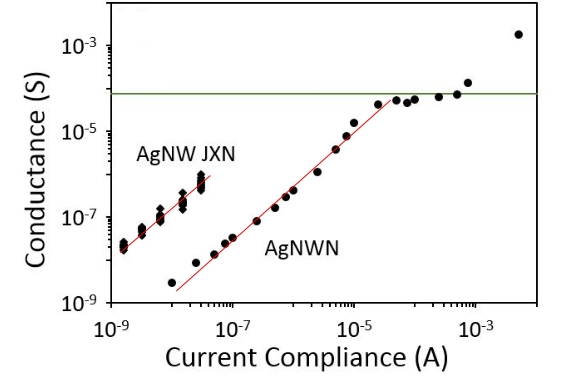
\includegraphics[width= 0.49 \columnwidth]{Images/Chapter5/exp_measurements.jpg}
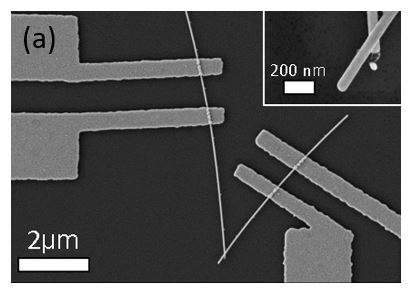
\includegraphics[width= 0.49 \columnwidth]{Images/Chapter5/single_jxn.JPG}
\caption{\fontsize{12pt}{11pt}\selectfont \textit{a) The results of recording conductance Vs current compliance for a NWN and an individual nanowire junction. An example of the experimental set-up to record the conductance of a single junction is shown in b). (c) get an image of the NWN.}}
\label{fig: exp_scaling}
\end{figure}


We assume that the conductance of each junction is bounded between the high resistance state ($10^4 k \Omega$) and the low resistance state ($13 k \Omega$). The low resistance state corresponds to $1/\Gamma_0$, where $\Gamma_0$ the quantum of conductance. Upon formation of an unbroken filament across the dielectric barrier between nanowires the width of said filament will be one atom wide. The conductance of a one atom wide wire is calculated as the quantum of conductance or $\Gamma \approx 7.75 10^{-5} S$. Individual nanowire junctions can reach the quantum of conductance at sufficiently high current levels. 

The parameter phase space for junction scaling fall into three main groups, supra-linear scaling ($\alpha_j > 1$), linear ($\alpha_j = 1$), and ($\alpha_j > 1$) sub-linear scaling ($\alpha_j < 1$). Figure BLAH shows the results of simulations with varying exponents and prefactors. The scaling exponent has a marked impact on the evolution of NWN conductance. The scaling of NWNs closely matches the scaling of individual junctions. 
\todo{image of different exponents and prefactors for same NWN.}
Effect of prefactor, the amount of current that can flow through a matured junction.

\section{Memristive Model}
In 1971 Leon Chua proposed a new circuit element known as the memristor, an element whos resistance depended on a set of state variables. The memristors behaviour is generalised with the expressions
\begin{align}
v &= \mathcal{R}(w,i)i \nonumber \\
\frac{dw}{dt} &= f(w,i) \label{eq: chua_memristor}
\end{align}
where $w$ is a set of state variables and $f$, $\mathcal{R}$ are general functions and can explicit functions in time. A rich population of theoretical memristors can be described that follow this general definition of a memristor. In their seminal paper Strukov et al presented a theoretical model for a system where its memristance is determined by an ion drift mechanism\cite{strukov2008}. The memristive characteristics of the model were similar to experements on a $TiO_x$ memristor where the change in resistance was modulated by the drift of Oxygen vacancies into a junction from a doped $TiO_{2-x}$ layer towards the undoped $TiO_2$ layer at the opposite end of the junction. The model used to describe this behaviour was
\begin{align}
V(t) & = \left[ R_{on} \frac{w(t)}{D} + R_{off}\left(1-\frac{w(t)}{D}\right) \right] I(t) \nonumber \\
\frac{dw}{dt} & = \mu_v \frac{R_{on}}{D}I(t)
\end{align}
where t is time, D is the width of the junction, $\mu_v$ is the ion mobility, I is the current through the device and V is the potential across the device. w(t) is a state variable and essentially represents the length of the doped part of the connecting junction, when $w(t) = D$ the system is in the low resistance state ($R_{on}$) and is in the high resistance state when $w(t) = 0$. 



Here the conductance scaling relationship in equation ... has been re-written in the usual format of memristors, showing that the derivative of the state variable of the CF length (w(t)) can be written as a general function of the junctions parameters.
\end{comment}
%============================================
\section{Modelling the Memristive Response of a Nanowire Junction}
\label{Sec: mrm_model}

Figure \ref{fig: exp_scaling}(a) presents experimental measurements of the conductance of individual Ag/PVP nanowire junctions for increasing current compliance, explained in chapter 1, as triangular data points. Also plot in Figure \ref{fig: exp_scaling}(a) is the conductance of an Ag/PVP NWN as circular data points\cite{scaling2018}. Here both the individual junctions and the NWN respond in a memristive manner to increasing current compliance, and these measurements reveal that their conductivity increases in a power law manner. The NWN scales with a power law over three decades of current compliance signified by the red line through the data points. Remarkably, the fitted power law to the NWN has the same exponent as the power laws fitted to the individual nanowire junctions, meaning their respective conductances ($\Gamma_{nt}$ and $\Gamma_{j}$) scale in a self-similar manner. The scaling of an individual junction is described with the power law
\begin{equation}
\Gamma_j = A_j I^{\alpha_j}
\label{eq: junction_pl}
\end{equation}
where the values of $A_j$ and $\alpha_j$ are material dependent and determine the memristive response of the material. While the memristive scaling presented in Figure \ref{fig: exp_scaling}(a) is particular to Ag/PVP nanowires, the self-similar scaling between junctions and networks was seen for a range of nanowire materials: Ni/NiO, core-shell Ag/TiO$_2$ and Cu/CuO\cite{scaling2018}. 

\fig{1}
{Images/Chapter5/exp_evidence.pdf}
{\textbf{Plot:} Conductance of a nanowire junction and network versus increasing current compliance.}
{(a) Experimental measurements of the conductance of individual Ag/PVP nanowire junctions (triangles) and an Ag/PVP NWN with increasing current compliance levels. Both systems display a power law scaling of the conductance; in the case of the NWN, this holds until a point at which the conductance reaches a plateau. (b) A magnified view of the memristive response of the NWN in (a) in the vicinity of the plateau where the conductance of the network $\Gamma_{nt}$ has been normalised by the quantum of conductance $\Gamma_0$. Here several smaller plateaus are observed with a conductance $\Gamma_p$ that are fractions of $\Gamma_0$\cite{scaling2018}. }
{fig: exp_scaling}

Another intriguing phenomenon is observed in the NWN conductance curve where it no longer scales as a power law and reaches a plateau. Figure \ref{fig: exp_scaling}(b) is a magnified view of this region where the fine detail can be seen. Three distinct plateaus in the network conductance can be seen, each represented by the horizontal orange and brown lines. The conductance of the network has been normalised by the quantum of conductance ($\Gamma_0 = 2 e^2/h$), the conductance of a single atomic channel that can transport a single spin degenerate pair of electrons, where $e$ is the charge of an electron and $h$ is Planck's constant. The plateaus have an approximate normalised conductance of $\Gamma_{nt}/\Gamma_0 \approx 1/8$ (bottom), $\Gamma_{nt}/\Gamma_0 \approx 1/6$ (middle), and $\Gamma_{nt}/\Gamma_0 \approx 1/5$ (top). Conductance plateaus were not seen for all of the examined NWN materials mentioned above meaning that specific material properties are required to observe them. In this section, a memristive model for individual nanowire junctions is introduced and used in the next section in a computational model of a memristive NWN. The computational model is implemented to explain the self-similar scaling between junctions and NWNs, and to understand the cause of plateaus in NWN conductance.

Nanowire junctions are described using the scaling law presented in equation \ref{eq: junction_pl}. The memristive response of a NWN is then determined through the collective response of the connected nanowire junctions. The set of parameters [$A_j,\alpha_j$] determines the response of each nanowire junction and are obtained from experimental measurements, $\alpha_j$ was found to fluctuate around $1$ depending on the materials involved in the junction\cite{scaling2018}. We assume that the resistance of the junctions are bounded by an initial high resistance state (HRS), or the off state, where $R_{off} = 10^4~ k \Omega$ was chosen as a suitably high value. The low resistance state (LRS) was assumed to correspond to the quantum of conductance $R_{on} = 12.9~k\Omega$ (equivalent to $1/\Gamma_0$). In planar MIM devices, the physical process responsible for decreasing resistance, often referred to as the state variable, is the formation of a conductive filament from electromobile atoms or ions that originate in the electrodes\cite{yang2012}. The growth of the conductive filament is regulated by distinct mechanisms including thermochemical, electrochemical metallization, and valence change\cite{memristors2014,lim2015,jeong2012,manning2017,waser2009}. Where a conductive filament mediates the resistance of the junction, one can assume that once it spans the entire insulating barrier between metallic cores that the conduction is through a single channel. A single conducting channel is a quantum of conductance and so approximates the conductance of a fully formed filament in our model. Thus, this empirical model referred to as power law plus cut-off (PL+C) describes the junctions whose conductance can vary with equation \ref{eq: junction_pl} but only in the range $[\Gamma_{off},~\Gamma_{0}]$.

Figure \ref{fig: single_nw_Aj_aj} presents the scaling of the conductance of a single junction with according to PL+C for distinct values of $A_j$ and $\alpha_j$. The effect of $A_j$ on junction conductance is plot in Figure \ref{fig: single_nw_Aj_aj}(a) where the scaling exponent is set $\alpha_j = 1$. Several effects of changing $A_j$ are seen in this plot, most notably increasing values shift the conductance curve to the left meaning that the junction begins to evolve at lower current levels but also reaches its ultimate conductance at a lower current. The current ($I_{th}$) at which a junction reaches its ultimate conductance $\Gamma_0$ is calculated as
\begin{equation}
\Gamma_0 = A_j (I_{th})^{\alpha_j} \rightarrow I_{th} = \left(\frac{\Gamma_0}{A_j}\right)^{\frac{1}{\alpha_j}} 
\end{equation}
The inverse relationship between $I_{th}$ and $A_j$ is visualised as the purple curve corresponding to the largest value of $A_j$ reaching $\Gamma_0$ first. Similarly, the current level where the junction conductance begins to increase ($I_{b}$) is obtained as
\begin{equation}
I_b = \left(\frac{\Gamma_{off}}{A_j}\right)^{\frac{1}{\alpha_j}} 
\label{eq:conductance_off_threshold}
\end{equation}
Here the inverse relationship between $I_b$ and $A_j$ is seen as the curve with $A_j = 0.5$ begins to increase in conductivity first.

The effect of different scaling exponents on the evolution of the junctions conductance is best understood by considering the derivative of equation \ref{eq: junction_pl}, which is the so-called strengthening rate $\nu_j$ 
\begin{equation}
\nu_j = \frac{d \Gamma_j}{dI} = A_j \alpha_j I^{\alpha_j - 1}
\label{eq: junction_pl_deriv}
\end{equation}
According to equation \ref{eq: junction_pl_deriv}, there are three distinct regimes of NWN scaling exponents. For a sub-linear exponent $\alpha_j <1$, $\nu_j$ decreases with current meaning that further increasing the conductance becomes more difficult. For supra-linear exponents $\alpha_j > 1$, $\nu_j$ increases with current meaning that further strengthening the junctions becomes easier as they become more conductive. Finally the linear exponent case $\alpha_j = 1$ has a constant strengthening rate. Each of these exponents give rise to unique conductance curves and are presented in Figure \ref{fig: single_nw_Aj_aj}(b) where the prefactor is set to $A_j = 0.1$. As both axis are in log-scale, the difference in junction conductance scalings for the power-law exponents are clear. The change in critical current flow $I_{b}$ is also evident as the smaller exponent requires less current to begin conductance improvement.

\fig{1}
{Images/Chapter5/single_aj_alpha_combined.pdf}
{\textbf{Plot:} Junction memristance with varying prefactor and exponent.}
{(a) Effect of changing the prefactor $A_j$ on the evolution of the conductance of a single nanowire junction with scaling exponent $\alpha_j = 1$ for increasing current levels given in units of current (u.c.). (b) Effect of changing the scaling exponent on the conductance evolution for a nanowire junction with $A_j = 0.1$. The differing $I_{th}$ and $I_b$ are seen in both plots. Note that all junctions begin at a conductance of $\Gamma_{off} = 10^{-4}~\mu S$ and finish at a conductance $\Gamma_0 \approx 0.0775~ \mu S$, the upper and lower bounds for junction conductance.}
{fig: single_nw_Aj_aj}

Drawing an analogy with the ion-drift model first proposed by Strukov et al\cite{strukov2008}, $A_j$ and $\alpha_j$ can be related to the mobility of the diffusing charge-carriers in the junction and to the nonlinear effects caused by the strong electric fields present in the dielectric layer \cite{scaling2018} respectively. In their model, Strukov et al hypothesised that the memristance was modulated by an interfacial boundary between an undoped $TiO_2$ and a $TiO_{2-x}$ layer doped with oxygen vacancies. The electrical response of such a junction can be described as
\begin{align}
V(t) & = \left[ R_{on} \frac{w(t)}{D} + R_{off} \left( 1 - \frac{w(t)}{D} \right) \right] I(t) \nonumber \\
\frac{dw}{dt} & = \mu_v\frac{R_{on}}{D} I(t) 
\label{eq: ion-drift-eqn}
\end{align}
where t is time, D is the full length of the $TiO_2/TiO_{2-x}$ junction, $\mu_v$ is the mobility of the ions, $I$ is the current, and $V$ is the output potential of the device. The state variable $w$ is the length of the doped layer which modulates the resistance of the junction and can vary between $0$ and $D$. The resistance of the junction clearly varies between $R_{on}$ and $R_{off}$ depending on the value of $w$.

According to the PL+C model for the conductance scaling of a nanowire junction, the conductance is a dynamical quantity controlled by the current-flow. For each current value the corresponding cumulative charge through the junction is $Q_c = \int_{-\infty}^{t} I(\tau) d\tau$. Experimental measurements typically involve increasing the current from zero to some current compliance $I_c$, before decreasing the current to zero again\cite{scaling2018}, as seen in the pinched hysteresis curves that were shown in chapter 1. Therefore a small increment in $I_c$ yields a similar increment in the cumulative charge such that $Q_c \propto I_c$, or $Q_c = B I_c$ with $B$ being a constant. Therefore, without loss of generality, we can write the power law equation in terms of the cumulative charge 
\begin{equation}
\Gamma_j = A_j I_c^{\alpha_j} = A_j B^{\alpha_j} Q_c^{\alpha_j} = \tilde{A}_j Q_c^{\alpha_j}
\end{equation}

Consider the case of a linear scaling exponent, $\alpha_j = 1$. Where a junction has not reached its ultimate high conductance state the stable current flow is a result of non-resonant electron tunnelling where the conductance follows an exponential dependence on the tunnelling gap
\begin{equation}
\Gamma_j = \Gamma_0 e^{-\beta (D - w(t))}
\label{eq: gamma_def}
\end{equation}
where $\beta$ is a decay parameter that characterises the tunnelling barrier. As discussed in chapter 1, the state variable $w(t)$ in the case of an electrochemical metallisation (ECM) memristive junction represents the length of the conductive filament bridging the inter-wire junction such that $\Gamma_0 e^{-\beta D} = \Gamma_{off}$. Using the fact that $\frac{dw}{dt} \propto I(t)$ and an approximation for the exponential with small separations $D-w(t)$
\begin{equation}
\frac{d \Gamma_j}{dt} = \Gamma_0 \beta \frac{dw}{dt} = \tilde{A}_j \frac{dQ}{dt} = \tilde{A}_j I(t)
\label{eq: linear_state_eqn}
\end{equation}
The state equation that determines the growth of the filament is thus
\begin{equation}
\frac{dw}{dt} = \frac{\tilde{A}_j}{\beta \Gamma_0} I(t)
\end{equation}
Since $\Gamma_0 = 1/R_{on}$ we obtain the following relationship for $\tilde{A}_j$ by comparing equations \ref{eq: gamma_def} and \ref{eq: linear_state_eqn}.
\begin{equation}
\tilde{A}_j = \frac{\mu_v \beta}{D}
\end{equation}
This relates the prefactor $\tilde{A}_j$ (and consequently $A_j$) with the ion mobility, the electron decay parameter and the width of the junction.

The derivation up to now has assumed $\alpha_j = 1$, the effect of non-linearity in the charge carrier drift is manifested through $\alpha_j \neq 1$. Returning to equation \ref{eq: linear_state_eqn}, and not performing an expansion on the exponential in equation \ref{eq: gamma_def}, the general form of the state equation is
\begin{align}
\Gamma_j &= \Gamma_0 e^{-\beta (D - w(t))} = A_j Q^{\alpha_j} \nonumber \\
\frac{d \Gamma_j}{dt} &= \Gamma_0 \beta e^{-\beta(D - w(t))} \frac{dw}{dt}  = A_j \frac{d}{dt}(Q)^{\alpha_j} = A_j \alpha_j Q^{\alpha_j-1} I(t) \nonumber \\
\frac{dw}{dt} & = \frac{\mu_v}{D \Gamma_0} I(t) e^{-\beta(D - w(t))} \alpha_j (Q(t))^{\alpha_j -1}  =  \frac{\mu_v}{D \Gamma_0} I(t) f(W/D, \alpha_j, Q_c(t)))
\end{align}
The non-linearity of the scaling exponent is captured by the additional functional $f(\alpha_j,W/D, Q_c(t))$. Thus $\alpha_j$ can be interpreted as the non-linearity of the derivative of the state variable $w$, the length of the doped layer, on the driving current. While this analysis was particular to a $TiO_2$ material, the length of the doped layer. $w$ can be associated with the length of the conductive filament links the interpretation of $A_j$ and $\alpha_j$ to the conductive filament model.

In this section, experimental evidence for the memristive nature of nanowire junctions and NWNs was presented, and the PL+C model for nanowire junction memristance was introduced. In the next section, a computational routine to simulate networks of such junctions is described and used to understand the self-similar scaling and conductance plateaus in the NWN memristance.

%Thus the memristance of a non-linear NWN junction is expressed throught the equation
%\begin{align}
%V(t) & = \left[ R_{on} \frac{w(t)}{D} + R_{off}\left(1-\frac{w(t)}{D}\right) \right] I(t) \nonumber \\
%\frac{dw}{dt} & = \frac{\mu_v R_{on}}{D } I(t) e^{-\beta(D - w(t))} \alpha_j \left( \int_{\infty}^{t} I(\tau) d\tau \right)^{\alpha_j -1} 
%\end{align}

%Note that for $w(t) = D$ its derivative is $0$ as one expects. This result is analagous to other generalisations of the ion-drift model in which window functions are used to account for nonlinear effects that can exist at the boundaries of conductive channel and for the non-linearity of the state derivative on the driven current. (READ REFS ON THIS) 

%============================================
\section{Memristance in a Nanowire Network}
\label{Sec: mrm_network}
The PL+C model can be applied to a NWN by allowing the conductance of each junction in the network to vary with respect to current flowing through them. By solving Kirchhoff's set of linear equations, the potential of each wire $V_i$ in the JDA or each connection node in the MNR mappings is obtained, and using Ohm's law the current-flow through the junction is calculated. Consider a junction connecting nodes $m$ and $n$. Its conductance is given by $\Gamma_j^{mn}$, and the current-flow between the nodes ($\mathcal{I}_{\textit{mn}}$) is calculated as
\begin{equation}
\mathcal{I}_{\textit{mn}} = | V_\textit{m} - V_\textit{n}| \Gamma_j^{\textit{mn}}
\label{eq: current_flow}
\end{equation}
Knowing the current-flow, an updated junction conductance $\bar{\Gamma}_j^{\textit{mn}}$ can be calculated using the PL+C
\begin{equation}
\bar{\Gamma}_j^{\textit{mn}} = A_j \mathcal{I}_{\textit{mn}} ^{\alpha_j}
\label{eq: junction_update}
\end{equation}
This updating scheme must be applied recursively to every junction in the network once a change in sourced current through the network has occurred.

Before the computational routine is discussed in more detail, the different node voltage mappings MNR and JDA must be discussed in the context of memristive junctions. Recall that the MNR model scheme includes junction resistance ($R_j = 1/\Gamma_j$) and inner wire resistance ($R_{in}$) contributions interacting in a voltage-node network frame. While $R_j$ characterises a dynamical quantity in accordance to equations \ref{eq: junction_pl} and \ref{eq: junction_update}, $R_{in}$ is fixed and it is given by $R_{in} = \rho \ell/A_c$ where $\rho$ is the wire resistivity, $\ell$ is the wire segment length and $A_c$ is the cross sectional area of the wire. The inclusion of inner-wire resistance is not entirely necessary for these simulations of an Ag/PVP NWN, as the junction resistances will be between $10^7 -10^4 ~\Omega$ compared with the resistance of inner-wire resistance which is of the order of tens of $\Omega$. Therefore, as $R_j >> R_{in}$ the JDA model will suffice in producing $\Gamma_{nt} \times I_c$ curves. In the next section however, a method to visualise current-flow through the network is introduced. The visualisations are of current-flow through nanowire segments, and so the MNR model is required in this case. This point will be discussed further in the following section.

Simulations begin with the sourced current at some minuscule value and iterating it up to some predefined maximum value of $I_{max}$. At each current-step, the potential of each node in the network is calculated with Kirchhoff's matrix equation. The current flow through each junction is calculated according to equation \ref{eq: current_flow} and the junction resistances are then updated with equation \ref{eq: junction_update}. After each junction has been updated and the values stored in the Kirchhoff matrix ($M_R$), the conductance of the entire network ($\Gamma_{nt}$) is then calculated. Following this the current is iterated to a new value and the junction update routine is repeated. For the first iteration, $\Gamma^{\textit{nm}}_j = \Gamma_{off}$ $\forall\,\, (n,m)$ internode pairs and junctions are updated until they reach their maximum conductance $\Gamma_0$. The work-flow diagram of the computational model can be seen in Figure \ref{fig: model_workflow}.

\fig{0.5}
{Images/Chapter5/mrm_work_flow.pdf}
{\textbf{Diagram:} Workflow diagram of memristive model simulation.}
{Workflow diagram of the computational implementation of PL+C junction model onto macroscopic networks. The algorithm obtains the conductance evolution of NWNs subjected to an electrical current source. See main text for detailed explanation of the algorithm.}
{fig: model_workflow}

In order to remove random connectivity profile effects from determining the role of different $A_j$ and $\alpha_j$ combinations on the evolution of a network conductance, an identical digital NWN geometry was used for each simulation. An experimental sample of size $ 20\times 20~ \mu m$ with wires of average length $6.7 ~ \mu m $ and of density $0.49$ nanowires$/\mu m^2$ was digitised using the method outlined in chapter 3. Figure \ref{fig: NWN_sample}(a) is an SEM image of said sample. Figure \ref{fig: NWN_sample}(b) is a digitised version of the NWN where wires are represented by grey sticks and the electrodes as thick vertical yellow lines. Figure \ref{fig: NWN_sample}(c) is a visualisation of the connectivity profile that is obtained from the digitised geometry of the NWN. Black dots represent memristive nanowire junctions and the two yellow dots are the two electrodes. Note all dots are connected by straight lines which correspond to current carrying nanowire segments.

\fig{1}
{Images/Chapter5/NWN_sample.jpg}
{\textbf{Sketch:} SEM and digitised image of a NWN.}
{(a) An SEM image of a NWN made of Ag/PVP core-shell nanowires that have a mean length of $ 6.7~ \mu m$ and a network size of $20 \times 20~ \mu m$. This sample has a wire density of $0.49$ nanowires$/\mu m^2$. The bottom scale bar represents $10~ \mu m$. (b) Digitised version of the NWN in (a), the grey lines represent nanowires and the thick vertical yellow lines represent the electrodes. (c) A graphical representation of the digitised NWN geometry from (b). The electrodes are represented by the two yellow dots on either sides of the figure. Black dots are nanowire junctions and the straight black line segments that connect junctions are current carrying wire segments.}
{fig: NWN_sample}

Figure \ref{fig: NWN_exponents} presents the effect on the conductance curve evolution for different combinations of the parameters $A_j$ and $\alpha_j$. Even though the junction characteristics are well defined, how current will flow though a collective of these junctions and the resulting macro scale network conductance is not clear. As discussed in the previous section, there are three distinct parameter spaces that are determined by the exponent value; sub-linear, linear, and supra-linear exponents, and each are expected to have varying evolution characteristics. In Figure \ref{fig: NWN_exponents}(a), the conductance curves for exponent $\alpha_j= 0.9$ are shown for three different values of $A_j$. The left-most curve has the highest value of $A_j = 0.5$ and it decreases for each curve as one moves to the right. All panels have a common legend which is displayed at the top of panel (b). This behaviour is of course expected as recalling from equation \ref{eq:conductance_off_threshold}, $I_b \propto A_j^{\frac{-1}{\alpha_j}}$ and so the greater $A_j$ is, the lower the current a junction will begin to improve conductance at. Recall $A_j$ can be interpreted as the ease of conductive filament formation for the MIM material. Notice that the conductance curve gradually decreases in slope with higher current levels; the $A_j = 0.5$ curve in particular saturates at $I = 10 ~ u.c$ meaning that the majority of junctions are reaching the LRS.

Figures \ref{fig: NWN_exponents} (b) and (c) present the conductance curves for exponents $\alpha_j = 1$ and $1.1$ respectively, also with varying $A_j$ values in each case. The same behaviour is seen as before where systems with higher $A_j$ values begin to strengthen first. However, for linear and supra-linear junction dynamics, the smooth conductance growth seen for the sub-linear case is lost. In particular, for exponent $\alpha_j = 1.1$ in panel (c) after an initial power law scaling phase, the conductance growth is characterised by plateaus in $\Gamma_{nt}$ corresponding to an Ohmic response to increasing current punctuated by sudden increases in NWN conductance which shall be discussed in more detail later in this section. Similar to the sub-linear case the network conductance begins to saturate at high currents for $A_j = 0.5$ meaning that this behaviour applies to the three exponent regimes.

\fig{1}
{Images/Chapter5/NWN_exponent_fits_modified.pdf}
{\textbf{Plot:} NWN memristance for various junction prefactors and exponents.}
{The conductance versus current plots for the memristive response model applied to the network geometry outlined in Figure \ref{fig: NWN_sample}. Simulations with different values of $A_j$ and $\alpha_j = 0.9$ (Figure (a)), $\alpha_j = 1$ (Figure (b)), $\alpha_j = 1.1$ (Figure (c)), $<\alpha_j> = 1.05$ (Figure (d)). In the latter case the junction exponents in the NWN follow a truncated normal distribution with a mean value of $<\alpha_j>$, a standard deviation of 0.1, and is truncated at [1,1.1]. The black dotted lines represent fitted power laws to the PL regime of the $A_j = 0.01$ case for each exponent value and is slightly offset to the curve for ease of viewing. The prefactor and exponent for these power laws, along with these parameters for fits to each of the other conductance curves are presented in Table \ref{tbl: PL_parameters}. The horizontal purple lines shown in each figure represents the conductance of the optimal path between electrodes, where there are 4 junctions in their low resistance states connected in series $\Gamma = 1/4 \Gamma_0$. The number of junctions in the optimal path between electrodes were determined by Network analysis of Figure \ref{fig: NWN_sample}(c).\cite{scaling2018}}
{fig: NWN_exponents}

In panels (a)-(c) in Figure \ref{fig: NWN_exponents}, a dotted line representing a fitted power law is visible, slightly offset to the $A_j = 0.01$ curve for each exponent for visualisation purposes. This fitted curve has a slope of $\alpha_{nt} = 0.892$ in panel (a), extremely close to that of the exponent of individual junctions, i.e. $\alpha_j = 0.9$. In fact, this self-similar scaling between networks and junctions is seen for each ${A_j,\alpha_j}$ shown in Figure \ref{fig: NWN_exponents}, where the slope of the power law in each case agrees closely with the junctions slope of which the network comprises. This supports the experimental evidence for self-similar scaling presented in section \ref{Sec: mrm_model}. The prefactors $A_{nt}$ and exponents $\alpha_{nt}$ taken from numerical fittings to the conductance curves in Figure \ref{fig: NWN_exponents} is given in Table \ref{tbl: PL_parameters}.

\begin{table}
\centering
\begin{tabular}{| c | c | c | c | c |}
\hline
$A_j$ & \textbf{0.01} & \textbf{0.05} & \textbf{0.1} & \textbf{0.5} \\ 
\hline 
$\alpha_j = 0.9$ & \{0.0027,0.892\} & \{0.0027,0.892\} &\{0.0266,0.9\} & \{0.1407,0.925\} \\
\hline
$\alpha_j = 1$ & \{0.0025,1.0\} & \{0.0125,1.0\} & \{0.0251,1.0\} & \{0.13071,1.024\} \\
\hline
$\alpha_j = 1.1$ & \{0.0024,1.115\} & \{0.0125,1.115\} & \{0.0251,1.113\} & \{0.13941,1.159\} \\
\hline
$ <\alpha_j> = 1.05$ & \{0.0025,1.054\} & \{0.0125,1.049\} & \{0.0251,1.051\} & \{0.1323,1.071\} \\
\hline
\end{tabular}
\caption{ \fontsize{12pt}{11pt}\selectfont Network prefactor ($A_{nt}$) and scaling exponent $\alpha_{nt}$ for each combination of $A_j$ and $\alpha_j$ obtained from fitting power laws $\Gamma_{nt} = A_{nt} I^{\alpha_{nt}}$ to the conductance curves shown in Figure \ref{fig: NWN_exponents}. The prefactors and exponents are presented as \{$A_{nt},\alpha_{nt}$\} in this table\cite{scaling2018}.} 
\label{tbl: PL_parameters}
\end{table}

The horizontal purple dashed line represents conductance of four junctions in series that are in the low resistance state $\Gamma_p = \Gamma_0/4$. According to the graphical representation of the NWN sample the memristive model was applied to, which is shown in Figure \ref{fig: NWN_sample} (c), there are precisely four junctions in the shortest path between the two electrodes. This fact gives a clue as to the networks behaviour during and after the power law scaling. For the sub-linear and linear exponent simulations, the conductance curves begin to diverge away from the initial power law scaling in a gradual manner. In the supra-linear case, a plateau is seen at precisely $\Gamma_p$ suggesting that the network conductance is dominated by four low resistance state junctions in series. In this scenario all of the current in the NWN may be funnelled through a single low-resistance path, or a winner-takes-all (WTA) pathway. Further evidence of localised current-flow is that $A_{nt} \approx A_j/4$ for exponents $\alpha_j \geq 1$ in table \ref{tbl: PL_parameters}, except for the $A_j = 0.5$ case. This can be explained as four conductors in series scaling in unison with increased current flow
\begin{equation}
\Gamma_p(I) = \frac{A_j}{4} I^{\alpha_j} = A_{nt}I^{\alpha_{nt}} 
\end{equation}
This relationship for localised current-flow is manifested by the self-similar scaling and the fact that $A_{nt} \approx \frac{A_j}{4}$ for each of the simulations where $\alpha_j \geq 1$ bar the case with $A_j = 0.5$. The exact nature of current-flow through the network is further examined in the following section. 

Finally, in Figure \ref{fig: NWN_exponents}(d), the sheet conductance is calculated where a level of disorder is incorporated in the assignment of the junction exponents. Each junction in the NWN is assigned a scaling exponent from a normal distribution centred at $<\alpha_j> = 1.05$, with a standard deviation of $0.1$ and confined to the range [1,1.1]. Figure \ref{fig: NWN_exponents}(d) is the average conductance of an ensemble of ten NWNs whose junctions were randomly assigned scaling exponents, and similar to panels (b) and (c), there is a clear power-law scaling regime. The first plateau takes place at $\Gamma_p \approx \Gamma_0/4$, again suggesting the emergence of a WTA between electrodes. The black dashed line is the fitted power law $\Gamma_{nt} = A_{nt} I^{\alpha_{nt}}$ to the $A_j = 0.01$ simulation and it was found to have an exponent of $\alpha_{nt} = 1.054$, very close to the average junction exponent. The fitted parameters obtained for the power-law in the other prefactor simulations are shown in Table \ref{tbl: PL_parameters} and all have exponents close to $1.05$. 

In the linear and supra-linear scaling simulations in Figures \ref{fig: NWN_exponents}(b)-(d), distinct conduction regimes are evident for the studied networks. The different regimes are identified in Figure \ref{fig: scaling_regimes} for a simulation with $A_j = 0.05$ and $\alpha_j = 1.1$. The OFF regime is the initial Ohmic response of a NWN to low current levels where current flowing through junctions in the NWN are too low to begin the process of junction evolution. and so most of the junctions are still in the $R_{off}$ state. Following this is the initial evolution of the junctions in the transient growth (TG) regime which is characterised by a varying network strengthening rate corresponding to a varying non-linear increase in sheet conductance that tends to a power-law. The power-law (PL) regime is the portion of the networks behaviour where it scales with an exponent similar to that of the junction. The behaviour following the PL regime is known as the post-power-law (PPL) regime and appears as a divergence of the network conductance away from the power law and towards saturation. These conducting regimes are further explored in the following section.

\fig{0.75}
{Images/Chapter5/scaling_regimes.pdf}
{\textbf{Plot:} Scaling regimes of a NWN conductance a supra-linear junction exponent.}
{Network conductance ($\Gamma_{nt}$) versus current for a network with $\alpha_j=1.1$ and $A_j = 0.05$. There are four regimes of network conductance evident in this plot: the OFF regime corresponds to current levels that are not sufficiently large to begin junction evolution. The transient growth (TG) occurs where the network has a varying strengthening rate until it reaches the power-law (PL) regime that is characterised by a power-law with an exponent approximately that of the junctions. The first plateau occurs immediately after the PL regime and heralds the beginning of the post-power-law (PPL) regime.}
{fig: scaling_regimes}

%-------------------------------------------
\section{Current Colour Maps}
\label{Sec: current_colour}
A useful tool in understanding the nature of emergent memristance in a NWN is to calculate the current flow through every individual wire segment and plot it as a 'heat-map', where colour intensity corresponds to the amount of current-flow. Using the MNR model the current flowing through a wire segment bounded by connection nodes $m$ and $n$ is simply the voltage difference between the node pair divided by the resistance of that segment.
\begin{equation}
\mathcal{I}_{\textit{mn}} = \frac{|V_\textit{m} - V_\textit{n}|}{(R_{in})_{\textit{mn}}}
\end{equation}
At every iteration of the computational model, the current through each wire segment was recorded and used to generate the current colour maps. Figure \ref{fig: new_nwn_all_exponents} presents conductance for a network in three scaling regimes plus their corresponding current colour maps at three probing states. The current colour maps are linked to the conductance curve to the left via the symbols located at the top right of each map (star, triangle, and circle). Figure \ref{fig: new_nwn_all_exponents}(a) is the conductance curve for a network with $\alpha_j = 0.9$ with its current colour mappings to the right. The first mapping (I = 1.0 u.c.), linked with the star symbol, is set in the PL regime of this network. Here one can identify several paths through the network that are carrying the sourced current as the lighter paths set against the blue background. As the source current is increased to I = 3 u.c. (triangle), the current-flow intensifies through these main paths and additional paths begin to form through the network also. At I = 9.3 u.c. (circle), the network is well into the PPL regime and several paths are carrying the current across the network. Figure \ref{fig: new_nwn_all_exponents}(b) contains the conductance curve and current colour maps for a network with $\alpha_j = 1$. Here a similar behaviour to the sub-linear scaling simulation is seen; the current flow is distributed through several paths between the electrodes.

\fig{1}
{Images/Chapter5/new_sample_all_exponents.png}
{\textbf{Plot:} Conductance curves and current colour maps for difference junction exponents.}
{(Far left panels) Network conductance ($\Gamma_{nt}$) versus sourced current ($I$) curves taken for a Ag NWN made with PL+C junctions of Aj = 0.05 and distinct exponents: $\alpha_j = 0.9$ (top), $\alpha_j = 1.0$ (middle), and $\alpha_j = 1.1$ (bottom). The currents are expressed in units of current (u.c.). The symbols mark points in the curves in which current colour maps were taken. (Three right panels) Current colour maps calculated over each wire segment of the network. Snapshots were taken for three current values specified on the top of each current map and distinguished by the symbols: star (set in the PL regime), triangle, and circle (both set in a PPL regime)\cite{scaling2018}. }
{fig: new_nwn_all_exponents}

In the supra-linear simulation, Figure \ref{fig: new_nwn_all_exponents}(c), a striking difference is clear between it and simulations with smaller scaling exponents. In the PL regime, the current is predominantly flowing through a single pathway as opposed to the more distributed current-flow seen for $\alpha_j \leq 1$. The single path that emerges in the PL regime taken in conjunction with the fact that the first plateau occurs at a conductance $\Gamma_0/n$ where $n$ is the number of junctions in the path suggests the emergence of the winner-takes-all behaviour of supra-linear scaling NWNs. As the current is increased and the network enters the PPL regime, the origin of additional plateaus are associated with the emergence of additional paths between the electrodes. At the second plateau for instance, the network creates a second path that is entirely independent from the first. At I = 7 u.c. which is well into the PPL, other paths emerge and note that they overlap. The emergence of WTA paths leads to a unique behaviour in the network memristive response with the sequential emergence of highly conductive pathways across the network. Figure \ref{fig: 1.1_current_maps} is a closer examination of the current colour maps of a different network geometry at different points in the networks conductance strengthening. This figure presents the response of a NWN with memristive parameters, $A_j = 0.05$ and $\alpha_j = 1.1$. The network conductance is shown in Figure \ref{fig: 1.1_current_maps}(a) and conductance maps at various current levels are in panels (b)-(e). Each current scan is labelled with a different symbol (square, star, triangle, and circle) which is then connected with a position on the conductance curve. The square symbol on the conductance curve is at $I = 0.07$ u.c. and the corresponding current scan is visible in Figure \ref{fig: 1.1_current_maps}(b) which is a visualisation of the TG regime. The current-flow is spread throughout the network in order to transport current in the most energy efficient manner. In contrast, the power-law regime sees the emergence of a highly localised current flow through the network, which shows that the self-similar scaling between the junction and network conductance is indeed a consequence of the the current-flow confined to a single path between electrodes. The transient growth region can be understood as the network seeking out a particular path which emerges in the PL regime through which the majority of current flow occurs in a WTA manner. The current mapping for the first plateau is labelled with the triangle symbol and shows that the WTA path still dominates the conductance of the junction at this point. The constant conductance at this stage of the network's evolution means no junctions are increasing in conductance, i.e. they are temporarily Ohmic. The conductance of the NWN at this current level is approximately $\Gamma_0/4$ due to there being four junctions in their final high conductance state. The PPL current mapping shows that several other pathways have emerged in the network at higher current levels (circle). Here the paths in the PPL are not all independent a number of paths share a junction.

\fig{1}
{Images/Chapter5/alpha_1_1_current_maps.png}
{\textbf{Plot:} Current colour maps for supra-linear junction exponent.}
{(a) Conductance versus sourced current (I) calculated for an Ag-PVP NWN made with power law junctions of $A_j = 0.05$ and $\alpha_j =1.1$. The black dotted line is a power law with $\alpha_{nt} \approx 1.1$ displaying self-similarity between the NWN and junction. The symbols mark points in the curves in which current maps were taken, a mapping was made in four different scaling regimes of the NWN; the transient growth (square), the power law (star), the first plateau (triangle), and the post power law (circle) regimes\cite{scaling2018}.}
{fig: 1.1_current_maps}

The winner-takes-all response shown for supra-linear junctions has been demonstrated in many simulations of different geometries alongside the two examples shown here\cite{scaling2018}. In fact, an experimental technique to image electrically grounded nanowires in a network was performed on an Ag/PVP NWN that had been electrically driven into a plateau state\cite{scaling2018,gemmill2004}. Known as a Passive Voltage Contrast image, the wires that have a stronger electrical contact with either electrode in Figure \ref{fig: exp_wta} appear as dark areas in the image while the lighter coloured ones are not well connected electrically to the mesh\cite{scaling2018}. Here the localised dark wires indicate that this pathway is significantly more conductive than the surrounding nanowires which further evidences the winner-takes-all response of Ag/PVP NWNs.
\fig{0.75}
{Images/Chapter5/exp_wta.pdf}
{\textbf{Image:} A Passive Voltage Contrast image of a NWN evolved to a plateau in conductance.}
{A Passive Voltage Contrast image\cite{gemmill2004} of an Ag/PVP NWN of size $100 \times 100 ~ \mu m$ that has been electrically driven to a stable conductive state at a current compliance of $50 ~ \mu A$. The dark wires indicate a strong electrical connection with the electrodes seen to the top and bottom of the image. Scale bar represents $2 ~ \mu m$\cite{scaling2018}.}
{fig: exp_wta}

Thus far, the memristance response of a NWN has been shown for a two terminal electrode geometry, in which two electrodes span the network at its opposite ends. In the following section, a multi-electrode architecture is presented that allows for a greater exploration of a network response to winner-takes-all pathways.
%=================================
\section{Multi-terminal}
\label{Sec: multi_terminal}
\fig{0.8}
{Images/Chapter5/multi_terminal_network.png}
{\textbf{Schematic:} Visualisation of a multi-electrode device in a memristive network.}
{Visualisation of a multi-terminal network to enable the formation of multiple WTA paths on the network. The four terminals are represented by thick vertical red lines and the nanowires as grey lines dispersed throughout the device. Four electrodes creates 6 unique electrode pairs between which WTAs can be formed.}
{fig: multi_terminal_nw}

The emergence of WTA paths as highlighted in Figures \ref{fig: 1.1_current_maps} and \ref{fig: exp_wta} demonstrates the possibility of activating distinct conductance states in a complex network system and this phenomenon has potential for neuromorphic applications. To fully realise the potential of memristive NWNs as a neuromorphic device, an architecture that facilitates multiple input signals, i.e. rather than a 2-probe interrogation method, is required. A neuromorphic network requires numerous electrical signals of distinct modulations and amplitudes inputted via a multi-terminal configuration such as that shown in Figure \ref{fig: multi_terminal_nw}. Here the four terminals are represented by thick red vertical lines and the nanowires (grey sticks) are randomly dispersed over a reference area. The four terminal architecture is used as a means to study the effect that the formation of a WTA has on other areas of the network. This will be achieved by developing a WTA path between a given pairs of electrodes and then calculating its impact on the conductance of other paths formed between the other electrode pair combinations. The same multi-terminal device of Figure \ref{fig: multi_terminal_nw} is shown in Figure \ref{fig: multi_pair_check}(a) along with sketches of the six possible paths between the four electrodes, represented by lines of various colours and in two cases as dashed lines. Current is sourced and drained between two electrodes only; in this case these were electrodes A and C and the path being evolved will be referred to as $\overline{AC}$. Junctions were set to evolve with a supra-linear exponent $\alpha_j = 1.1$ in order to facilitate the emergence of a WTA between A and C. After each increment in the sourced current along the path $\overline{AC}$, the conductance of every junction in the NWN is recalculated according to PL+C junction model and the resistance of probed by every electrode pair in the network is then calculated. 

\fig{1}
{Images/Chapter5/multi_terminal.pdf}
{\textbf{Plot:} Memory states in a multi-terminal NWN device.} 
{(a) A sketch of a multi-terminal NWN with 4 electrodes depicted by vertical red lines (labelled A-D), and light gray lines representing the nanowires. The paths between the terminals are depicted by thick lines of different colours. (b) The inter-electrode terminal for each of the 6 paths depicted in (a). The path between A and C is matured to a high conductance state corresponding to a new memory state while the memory states of the other paths change very little.}
{fig: multi_pair_check}

Figure \ref{fig: multi_pair_check}(b) plots the conductance of each electrode pair in the NWN that was shown in Figure \ref{fig: multi_pair_check}(a) while the current sourced at electrode A and drained at electrode C is incremented. The main path $\overline{AC}$ sees its conductance increase in a manner typical to two-terminal networks seen in previous section, a well defined PL regime and plateaus that indicative of WTA behaviour. While the other paths in the network were not explicitly evolved by running current through them, their conductances changed as a result of the WTA path $\overline{AC}$ nonetheless. The paths $\overline{AB}$ and $\overline{BC}$ saw an increase in their conductance by over $100\%$ while the paths $\overline{CD}$ and $\overline{AD}$ saw an approximately $30\%$ increase in conductance. The path $\overline{BD}$ which is represented by the green line saw hardly any change in its conductance which is interesting as it is the only path in the NWN that is independent of the electrodes A and C. The negligible change in the path $\overline{BD}$ also explains the change of conductance observed in the other non-driven paths. The evolution of the main path between the electrodes A and C causes a change in conductance for any other path containing these electrodes.  

While the multi-terminal device simulated in Figure \ref{fig: multi_pair_check} is a proof-of-concept, it does offer valuable insights into the potential of NWNs as a neuromorphic device. The contamination of non-driven paths by the evolution of a memory state in other paths is undesirable in memory storage devices and device architecture would need to mitigate this. This could be achieved through a large number of electrodes orientated in such a way so that shared junctions in their WTA is unlikely and when it does occur, contamination is minimal. The cross-contamination between memory states does have a novel application in neuromorphic devices as they are a means to achieve associative memory states\cite{pershin2010}, for example two paths, $\overline{AB}$ and $\overline{BC}$, doubled in conductance as a result of the formation of the WTA in $\overline{AC}$. Associative memory states means that the development of one memory state has an impact on another, leading to a computational system of high complexity and computational capabilities. This point will be discussed further in the Conclusions and Future Work chapter.

%-=============================
\section{Chapter Summary}
\label{Sec: mrm_conclusion}
In section \ref{Sec: mrm_model}, a model was introduced that empirically captured the memristive properties of a nanowire junction named as power-law plus cut-off (PL+C). This model was developed based of experimental measurements of nanowire junctions which showed a power law relationship between their conductance ($\Gamma_j$) and the current compliance such that $\Gamma_j = A_j I^{\alpha_j}$ where the parameters $A_j$ and $\alpha_j$ are determined from the experimental measurements. The upper bound for a junctions conductance was taken as the quantum of conductance, the conductance of a single channel connecting the nanowires, while the lower bound for conductance was set as $10^{-7}~ S$. These bounds are not fixed parameters and can be changed in accordance with the system being studied, here they were motivated by experimental data. The dynamics of the conductance evolution of a nanowire junction was shown to depend sensitively on the parameters $A_j$ and $\alpha_j$, mainly through the current level at which their conductance starts increasing from $\Gamma_{off}$ and when it ceases evolution at $\Gamma_{on}$.

A method to incorporate the dynamical junction resistance into the Kirchhoff's circuit equations was presented in section \ref{Sec: mrm_network} resulting in the capability of simulating the macro-scale memristance of a NWN based on the underlying memristive junctions. The network memristance was shown to have three main scaling dynamics depending on the value of the junction scaling exponent $\alpha_j$: sub-linear, linear or supra-linear. In all three cases a self-similar power law was identified between the scaling of junctions and networks comprised of these junctions. For supra-linear cases the emergence of highly conductive paths that display a winner-takes-all behaviour was evidenced by the appearance of a steady-state of the NWN conductance. Here the network entered a period of inactivity at a conductance corresponding to a single path of fully evolved junctions funnelling all of the current along it. Current colour mappings were introduced in section \ref{Sec: current_colour} as a means to visualise the current-flow through a NWN and further suggested the emergence of WTA paths during network evolution. Passive Voltage Contrast SEM images of a physical NWN that had undergone memristive evolution highlighted areas of highly conductive pathways that shows the winner-takes-all behaviour predicted by simulations.

A multi-electrode architecture for a NWN was introduced in section \ref{Sec: multi_terminal} such that several addressable inter-electrode paths could be interrogated while one of the paths was driven to a high conductance state. as expected, the main path saw an increase of over two orders of magnitude in its conductance as a winner-takes-all path was formed between the two driven electrodes. Other paths in the NWN did not see such a dramatic increase in conductance, no more than a factor of two. One pathway did not increase in conductance whatsoever meaning that it was unaffected by the formation of the high conductance winner-takes-all. These results suggest that several independent addressable memory states could be stored in a NWN. The results also hint at a process to achieve associative memory states in a NWN through the use of shared electrodes, a remarkable property of a randomly connected set of nanowires. More tests and simulations need to be performed in order to exploit the full potential of this proof-of-concept neuromorphic random NWN device.
%==============================
\begin{comment}
\section{Transient Regime Dynamics}

\begin{figure}[htbp]
\centering
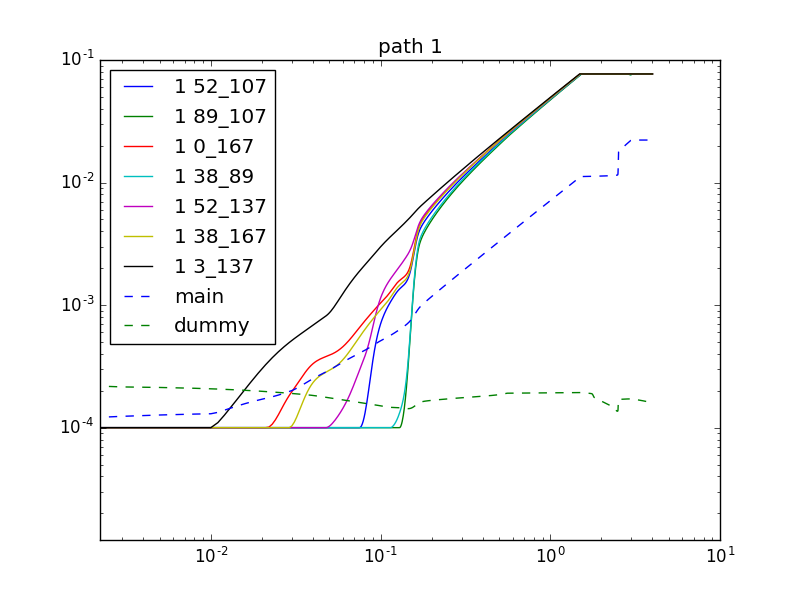
\includegraphics[width= 1 \columnwidth]{Images/Chapter5/path_1.png}
\caption{\fontsize{12pt}{11pt}\selectfont \textit{All the junctions in the main path between terminals. Main and dummy conductance shown in dotted lines}}
\label{fig: dummy_current_junctions}
\end{figure}


\section{Dummy current}
\begin{figure}[htbp]
\centering
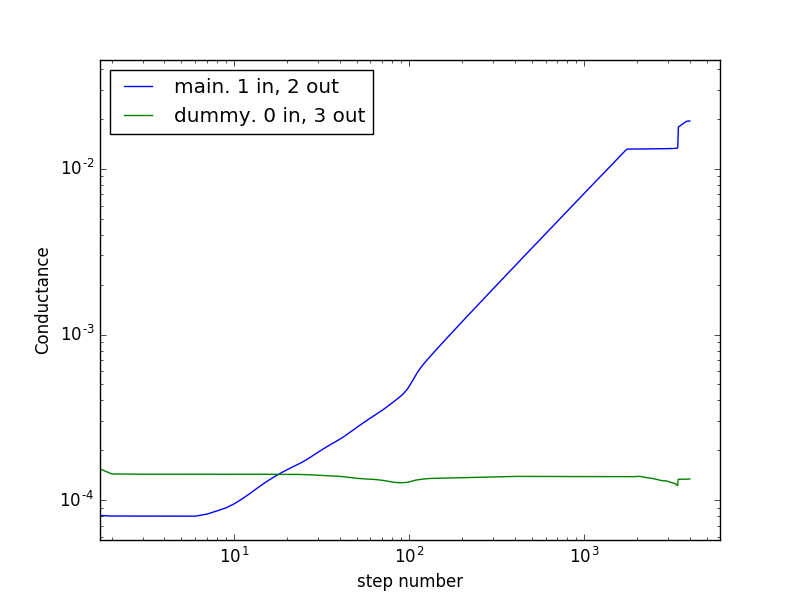
\includegraphics[width= 1 \columnwidth]{Images/Chapter5/min_1_mout_2.png}
\caption{\fontsize{12pt}{11pt}\selectfont \textit{Current is ramped up between the main electrodes, a small amount of current is extracted from the dummy terminals.}}
% Image from /home/colin/Dropbox (CRANN)/PhD/model/multi_terminal/4_terminal_pump_probe/1.1_exponent
\label{fig: dummy_current_main}
\end{figure}

A regular current scan occurs between two of the terminals, a small amount of current is passed in and out of the remaining two terminals. The conductance between the two dummy electrodes is also shown in Figure \ref{fig: dummy_current_main}. Two areas of note can be seen in the dummy conductance, namely the dip just before the PL regime in the main conductance curve and just at the end of the first plateau. In order to understand these features it is neccesary to examine the conductance of each individual junction in the main conductive path. These are shown in Fig \ref{fig: dummy_current_junctions}

\begin{figure}[htbp]
\centering
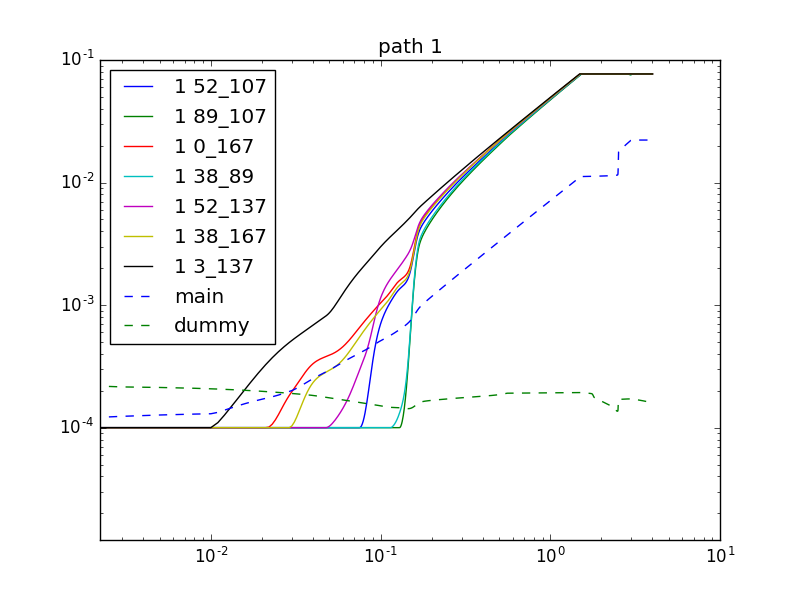
\includegraphics[width= 1 \columnwidth]{Images/Chapter5/path_1.png}
\caption{\fontsize{12pt}{11pt}\selectfont \textit{All the junctions in the main path between terminals. Main and dummy conductance shown in dotted lines}}
% Image from /home/colin/Dropbox (CRANN)/PhD/model/multi_terminal/4_terminal_pump_probe/1.1_exponent
\label{fig: dummy_current_junctions}
\end{figure}



The movement in the dummy current coincides with an initial period of conductance evolution in the junctions of the main conductive path between the main electrodes. This activity has a knock-on which manifests in the conductance of the dummy electrodes.

\section{Commutability and associativity}
It is clear from Figure \ref{fig: multi_pair_check} that the training of one path has an impact on the conductance state of other terminal pairs. Another examination for this is two test the commutability of training memory states in a NWN. First a conductance scan is performed on one pair of terminals. Any junctions that have reached an on state are fixed at this conductance value, any other conductances are allowed to reset to the off conductance state. In the case of two independant paths, i.e no terminal is used in both paths, one sees a definite commutability of memory states. The formation of one of the paths in this network has little effect on the formation of the second path. There is a slight difference in behaviour at the start of conductance scan but the latter behaviour, particularly the PL and plateau behaviour is the same for both scans. 
\begin{figure}[htbp]
\centering
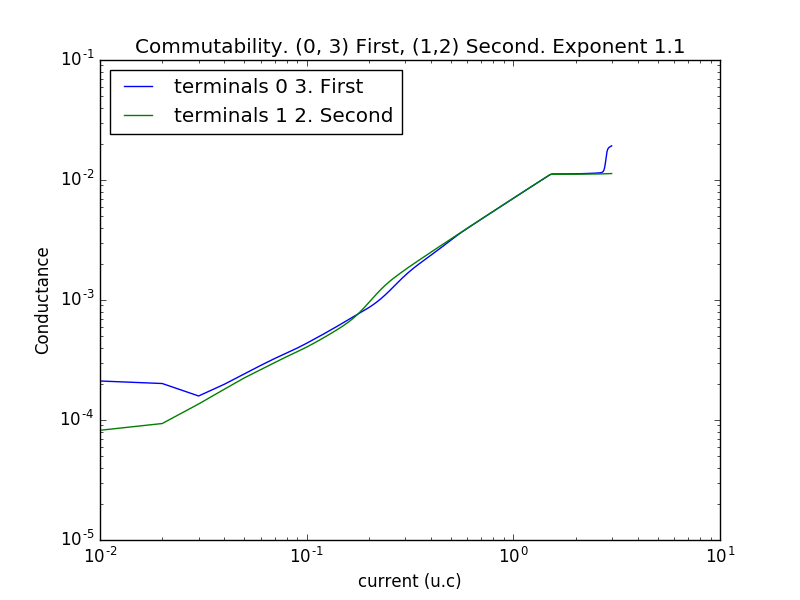
\includegraphics[width= 0.49 \columnwidth]{Images/Chapter5/0_3_f_1_2_s_expon_1_1.png}
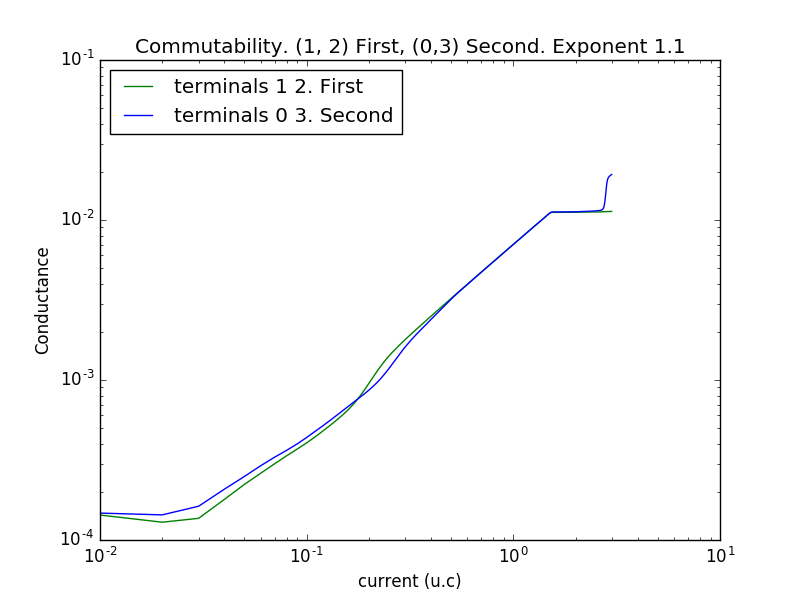
\includegraphics[width= 0.49 \columnwidth]{Images/Chapter5/1_2_f_0_3_s_expon_1_1.png}
\caption{\fontsize{12pt}{11pt}\selectfont \textit{Commutability }}
% Image from /home/colin/Dropbox (CRANN)/PhD/model/multi_terminal/commutability/density_0.5/network_1/network_1_seed_0_no_update
\label{fig: commutability}
\end{figure}
Figure \ref{fig: Associativity} shows the effect of a shared electrode on the commutability of path formation. There is a clear effect of the order of training on the final conductance states of the paths. The plot of the difference of the two conductance curves best illustrates this. These simulations highlight the effect of independent and shared terminal paths. An application of these different terminal layouts are as independent memory states, in the case the first case, and as associative memory in the latter.
\todo{add in plot of first scan - second scan}
\begin{figure}[htbp]
\centering
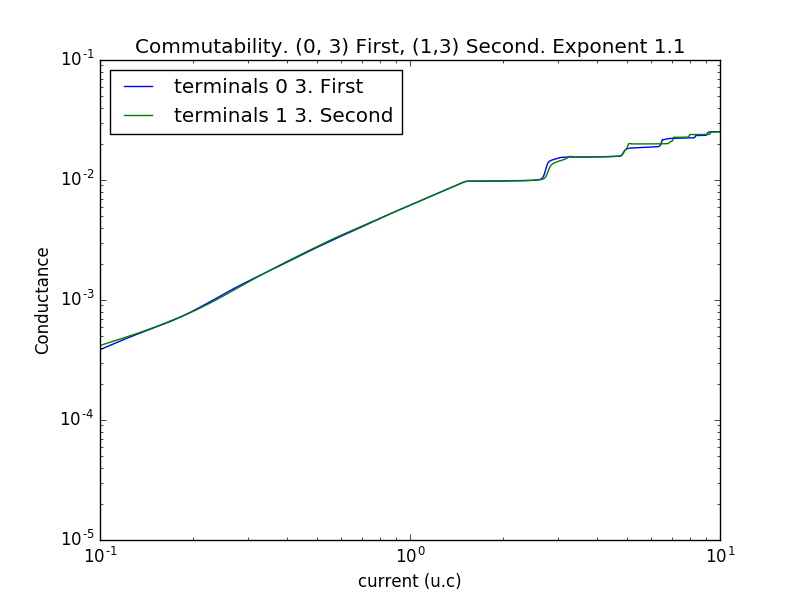
\includegraphics[width= 0.49 \columnwidth]{Images/Chapter5/associative_0_3_f_1_3_s_expon_1_1.png}
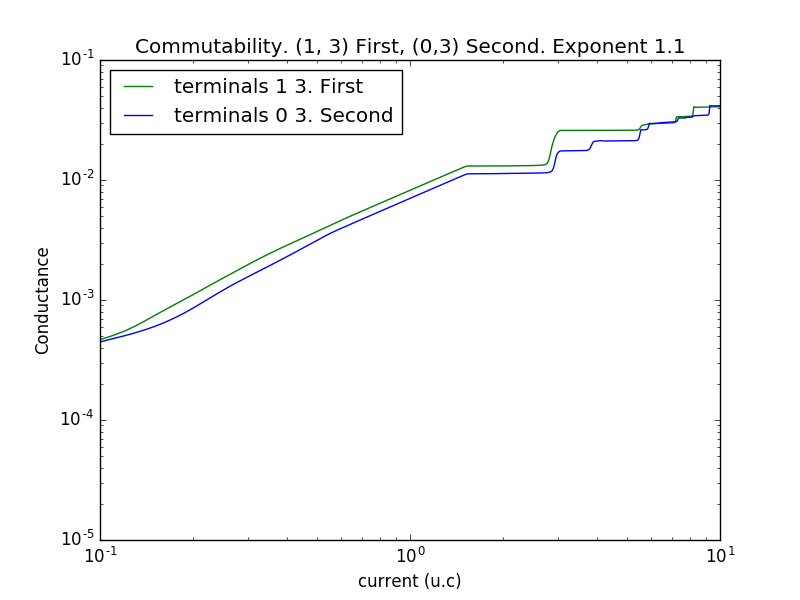
\includegraphics[width= 0.49 \columnwidth]{Images/Chapter5/associative_1_3_f_0_3_s_expon_1_1.png}
\caption{\fontsize{12pt}{11pt}\selectfont \textit{Commutability }}
% Image from /home/colin/Dropbox (CRANN)/PhD/model/multi_terminal/commutability/density_0.5/network_1/network_1_seed_0_no_update
\label{fig: Associativity}
\end{figure}
\end{comment}

%\bibliographystyle{ieeetr}  %%for ordered citations
%\bibliography{bibliography}

 \chapter{Comparison of a Capacitive and Memristive Junction Activation Process}
In the previous chapter, the memristive activation of a NWN undergoing electrical stressing was introduced. This junction activation is a current driven process that requires increasing current levels through the NWN, causing the conductance of each junction to change in an analogue manner up until their final high conductance state. It was also shown that the PL+C model has activation patterns that are highly dependent on the properties of the junction; for supra-linear junction scaling the emergence of highly localised current flows through the networks takes place in a `winner-takes-all' (WTA) manner, while for linear and sub-linear exponents, current-flow deviates from the WTA behaviour by distributing the current throughout the network. The PL+C is not the only contemporary model that describes the dynamical activation of nanowire networks however. In recent publications the inter-wire junctions have been treated as a capacitor which breaks down when the potential across the junction reaches some critical value, causing an electrical connection between the nanowires\cite{nirmalraj2012,fairfield2014,fairfield2016}. The capacitive model (CPM) for junctions has been used to identify the activation voltage of the network, i.e the voltage required to begin current flow through the network. At the point of network activation, a shorting path between two electrodes is fully formed, facilitating current flow between sources. From here on, the PL+C model shall be referred to as the memristor model (MRM).

\fig{1}
{Images/Chapter6/fig1_sketch.png}
{\textbf{Sketch:} A sketch of MRM and CPM junctions in a NWN along with PVC images of NWN displaying a capacitive and memristive response.}
{(Top panels) Circuit sketches representing a NWN being described by a (a) capacitive model (CPM) and a (b) memristive model (MRM). Each lumped circuit element is assigned to model the electrical characteristics of the interwire junctions in their respective formation (capacitors) and adaptive conducting (memristors) modes. Horizontal green lines represent metallic electrodes. (Bottom panels) PVC SEM images of Ag NWN samples subjected to distinct electrical characterizations. In (c), the image was taken by holding the source voltage at 2 Volts and setting a leakage current of few hundreds of pA. The network dimensions are 200 x 200 $\mu$m and the white scale bar corresponds to 20 $\mu$m. In (d), the image was taken from a full I-V sweep with a limiting current compliance of 500 nA. The network dimensions are 100 x 100 $\mu$m and the white scale bar corresponds to 2 $\mu$m. Darker wires are grounded to the electrodes meaning that their junctions were optimized in response to the given excitation. Almost the whole network is featured in the capacitive/formation regime whereas a single WTA path is contrasted in the memristive/conducting regime\cite{ocallaco2018}. More details on this experiment can be found in our publication\cite{ocallaco2018}.}
{fig: intro-fig}

The expected response of the network to a capacitive junction breakdown activation model is hinted at in Passive Voltage Contrast (PVC) images performed at low leakage current levels. Figure \ref{fig: intro-fig} (c) presents a PVC image of a nanowire network exposed to very low leakage current (hundreds of $pA$). In this image the dark wires represent those that have the strongest electrical connection with the electrodes. This leakage current is too low to begin the memristive evolution of the junctions which remain in their pristine insulating state, equivalent to a parallel placte capacitor. Figure \ref{fig: intro-fig}(d) is a PVC image performed at $500$ $nA$, a level at which memristive evolution has begun and here a localised electrical connection is depicted by the dark wires and is a manifestation of the WTA behaviour discussed in the previous chapter. These images suggest that networks will behave differently in the CPM and MRM. These behaviours will be compared in this chapter.

The aim of this chapter is to introduce and characterise certain traits associated with the CPM and contrast this with the dynamics of networks undergoing memristive activation. This is achieved by applying the CPM and MRM to an identical network geometry, as sketched in Figures \ref{fig: intro-fig}(a) and (b). Nanowires connected by either capacitive or memristive junctions are complementary models whose applicability depends on how the networks are interrogated. The capacitive response is dominant when the network is interrogated by extremely low currents ($\sim$ pA); in this regime, each junction is represented by a capacitor which breaks down if the voltage drop across it exceeds its characteristic threshold voltage making an electrical contact between the wires. Once this occurs, the junction becomes a memristor at a high-resistance state (HRS) and sufficiently small currents can flow through it. As more current is adiabatically sourced onto the network, the memristive state of these junctions can be continuously evolved up to their respective low-resistance state (LRS). 

This chapter will highlight the main difference between the activation of a network with binary state junctions (CPM) and analogue state junctions (MRM). The layout of this chapter is as follows. The capacitive junction model along with the computational framework to apply it to a NWN is introduced in section \ref{Sec: cap_comp_model}. The activation patterns of the CPM is illustrated in section \ref{Sec: mrm_cpm_activations} and here it is contrasted with that of the MRM by applying both to an identical network geometry. In section \ref{Sec: cpm_avalanches}, the CPM is shown to have a scale free response to network perturbation resulting in mass junction activation events that can propagate across the entire network. The fault-tolerance attribute of networks in both activation models are contrasted in section \ref{Sec: fault_tol} by examining junction activations and network performance after a junction that is central to the network performance `fails`, or is removed from the mathematical graph describing the NWN. There is a chapter summary presented in section \ref{Sec: cpm_conclusion}. 


%Our findings highlight the main differences between a breakdown-based switching process (involving binary capacitive transitions) and an gradual switch (involving analogue memristive components) in complex NWN systems. NWNs made of slow-switching elements exhibit a continuous spectrum of conductance states bounded only by the junction cutoffs  $\Gamma_{\textrm{off}} = 1/R_{\textrm{off}}$ and $\Gamma_{\textrm{on}} = 1/R_{\textrm{on}}$. This mechanism is shown to be highly selective, funnelling most of the sourced current through a single path (WTA state) of NWs bridging the electrodes. NWNs composed of fast-switching elements are not as selective however, with a much larger number of junctions playing an active role in forming a pathway between electrodes. We show that NWNs containing fast-switching elements evolve in a discrete fashion with the system alternating between stages of idleness and activity. While active, one can characterize the network dynamics by computing cascade events (or avalanches) comprised of clusters of junctions being activated simultaneously and their respective time durations. On the other hand, slow-switching junctions undergo a whole spectrum of conductance levels as the network is gradually excited by the current source. In this way, a binary cascade-like characterization cannot be conducted without the consideration of a (arbitrary) threshold parameter that classifies the occurrence (or not) of an avalanche event.
%Networks of slow-switching elements do not form a critical structure and so no such cascade events are observed. Furthermore, we show that the slow-switching dynamics are fault-tolerant in response to perturbations, i.e. the network transport response is robust against junction failure. Only a minute increase in sheet conductance occurs at the moment a WTA path activation is slightly perturbed in the network. The fast-switching dynamics however are susceptible to larger-scale junction failures, requiring up to 55\% additional switching events to form a continuously active pathway between electrodes.   

%===============================================================================

\section{Capacitive Junction Model}
\label{Sec: cap_comp_model}
The capacitive model is relevant to negligible current flows through the network such that the capacitive response of junctions dominates the network properties. In this scheme, the nanowires are treated as equipotential wire segments and their connections as binary capacitors. This modeling scheme is similar to the JDA approach introduced in chapter 3 in that the junctions define the connectivity profile of the network. This assumption was taken as charge can easily move through the conductive nanowire but not across the insulating barrier in a junction. Depending on the voltage drop across the capacitive junction, it can be either non-activated ($\ket{0}$) or activated ($\ket{1}$). The capacitance state of a junction can flip from $\ket{0}\rightarrow \ket{1}$ if the voltage drop across it is larger than its associated breakdown voltage ($V_b$), hence a given junction connecting a pair of wires $(n,m)$ can be activated if $|V_\textit{n} - V_\textit{m}| \geq V_b$ where $V_\textit{n}$ ($V_\textit{m}$) is the potential at wire $n$ ($m$). The capacitor activation is characterized by a modification in the capacitance value of the junction as $C_{\textit{nm}}^0 \rightarrow C_{\textit{nm}}^1$ where $C_{\textit{nm}}^0$ is an estimated quantity determined uniquely by the characteristics of the wires and $C_{\textit{nm}}^1\rightarrow 0$ meaning that the junction has lost its capacitive properties and charge will start to flow through it. The values of $C_{\textit{nm}}^0$ are estimated by considering interwire junctions as parallel-plate capacitors with $C_{\textit{nm}}^0 = C^0 = \epsilon_r \epsilon_0 A/d$ $\forall$ $(n,m)$ pairs for the sake of simplicity. In the equation, $\epsilon_r$ is the relative permittivity of the dielectric, $\epsilon_0$ is the permittivity of the air, $A$ is the plate area, and $d$ is the plate separation. For our PVP coated Ag nanowires, we used $\epsilon_r\approx 2.5$, $d\approx 8$ nm and the area of the plates can be estimated from the nanowire diameters which range $D\sim 60-80$ nm. Assuming an ideal square area projected from two superimposed soft-body wires, $A=D^2$ resulting in $C^0 \approx 18$ attoFarads (aF). The capacitance of wire sections is not considered by the CPM due to it being negligible for metallic core nanowires. If the CPM was applied to non-metallic wires the CPM should be extended to account for the coupling capacitance of the wires themselves.

CPM simulation \cite{fairfield2016} begins by placing the whole capacitor network in contact with electrodes that source and drain a certain amount of charge $Q$, representing the charge that builds up due to the applied bias voltage. The applied charge is incremented from an initial value $Q_i$ up to a pre-defined maximum value of $Q_{\textrm{max}}$ in steps of $\Delta Q$. At $Q_i$, all junctions are set at $\ket{0}$-state, and at each charge increment the electric potential of each wire is calculated and the potential difference across each junction is checked against the breakdown voltage. A capacitance matrix $\hat{M}_c$ is built taking into account the network connectivity and the potential on each wire is obtained by solving the system of equations $\hat{M}_c \hat{V} = \hat{Q}$ self-consistently. This means that charge on the electrodes is only incremented once all $\ket{0}\rightarrow \ket{1}$ transition activity on the network ceases. A work-flow schematic of the recursive CPM is shown in Figure \ref{fig: cpm_workflow}.

\fig{0.6}
{Images/Chapter6/cpm_work_flow.pdf}
{\textbf{Schematic:} A work-flow diagram of the capacitive junction model.}
{A workflow diagram of the capacitive junction model. Refer to the main text for fetails on the algorithm.}
{fig: cpm_workflow}

%At low current levels corresponding to the OFF-threshold in MRM, one can expect to find a capacitive response from the individual NW junctions coupled with some leakage current since their dielectric coating are not expected to be an ideal insulator; a small DC current can always leak through the dielectric material. For example in the passive voltage contrast image in Figure \ref{fig: intro-fig}(c) the leakage current was of the order of hundreds of pA ($10^{-7}A$).  To account for this dual response, CPM is modified to incorporate leakage current in capacitive networks by considering a parallel RC circuit as a proxy for low current flow in NWNs. A potential difference that is placed across both elements then links the charge accumulated on the NWN with a leakage current through the resistor. The size of the leakage resistor is chosen in order to give leakage currents of the order of hundreds of pA.
%The resisitor placed in parallel can be chosen in order to give a leakage c To simulate leakage currents of the order of pA, the resistance of this dummy resistor connected in parallel to the capacitive network ($R_d$), in this case we used $R_d\sim 10^{10}\,\Omega$.

The MRM follows the algorithm that was laid out in Chapter 5. For the sake of consistency, CPM and MRM were employed on the same NWN skeleton. By using an identical network geometry for both MRM and CPM simulations, the spatial fluctuations can be removed allowing a more direct comparison between the activation dynamics of both models. Figure \ref{fig: sample_nwn}(a) is a SEM image of a NWN sample made with Ag/PVP core-shell nanowires. This NWN has a wire density of 0.47 nanowires/$\mu$m$^2$ and the average length of the wires is approximately $7\, \mu$m. After digitally capturing the geometry of this network using the method introduced in chapter 3, we estimate that this network contains a total of 963 junctions. Figure \ref{fig: sample_nwn}(b) shows a stick representation of (a) which was built from the resultant graph\cite{rocha2015}. 

\fig{1}
{Images/Chapter6/sample.png}
{\textbf{Sketch:} An SEM image of a network and alongside its digitised counterpart.}
{(a) SEM image of an Ag NWN with a wire density of 0.47 nanowires/$\mu$m$^2$ and average wire length of $7~ \mu$m. Electrodes are located at either sides of the network and the white scale bar at the bottom represents 10 $\mu$m. (b) Stick representation of the Ag NWN sample taken from (a). Black sticks represent the Ag nanowires whereas the vertical thick green lines represent the electrodes\cite{ocallaco2018}.}
{fig: sample_nwn}

The CPM model is meant to capture the dynamics of the network at extremely low current levels while the MRM is applicable at higher levels. That being said, the two models are mutually exclusive in this thesis, they do not interact and there is no consideration of a dual memcapacitive and memristive response. There are reports of a memcapacitive and memristive response existing on nanoscale junctions\cite{hartmann2017,maier2016,wakrim2016,liu2006} but as the models are applied to current regimes orders of magnitude in difference, they were studied in isolation in this work. The dual memcapacitive/memristive properties of a nanowire junction is a potentially fruitfull area worth investigating and will be a subject of future work.
%========================================================================================================================
\section{Path Formation in Capacitive and Memristive Models}
\label{Sec: mrm_cpm_activations}
Recall from chapter 5 that the hallmark of supra-linear junction scaling was the emergence of winner-takes-all paths between the electrodes. The network geometry shown in Figure \ref{fig: sample_nwn} was set to evolve in accordance to the MRM outlined in chapter 5 from which $\Gamma_{\textrm{nt}} \times I$ curves were obtained. Figure \ref{fig: conductance_activated}(a) presents the evolution of the network conductance with junctions scaling according to equation \ref{eq: junction_pl} with $A_j = 0.05$ and $\alpha_j = 1.1$. The four scaling regimes identified in chapter 5 are labeled in this plot, the initial OFF state, the transient growth (TG) where the network identifies the winner-takes-all path and begins its power-law (PL) scaling. As discussed in chapter 5, the network conductance scales as $\Gamma_{nt} = A_{nt} I^{\alpha_{nt}}$ in a self-similar manner to the junctions, i.e. $\alpha_{nt} \approx \alpha_j$. Finally the network enters the post-power-law (PPL) regime where the winner-takes-all path is fully developed and additional paths are fully activated as the current flowing through the network continues to increase. 

\fig{0.6}
{Images/Chapter6/fig3_lines.png}
{\textbf{Plot:} Wire activation during NWN memristance increase for supra-linear junction exponent.} 
{(a) Simulated conductance versus current obtained for the image processed Ag NWN shown in Figure \ref{fig: sample_nwn}. The curve was calculated with the MRM. All four distinct transport regimes discussed on the main text is depicted on panel and highlighted in different colours: (OFF) OFF-threshold, (TG) transient growth, (PL) power law, and (PPL) post-power-law. Currents are expressed in units of current (u.c.). The junction characteristics are set at $\alpha_j=1.1$ and $A_j$ = 0.05. The blue circle marks the point in the curve in which the junctions comprising the WTA paths are fully optimised at $I = 1.77$ u.c. and  $\Gamma_{\textrm{nt}} = 0.013$ mS. This point marks the disruption of the PL conducting regime. (b-c) NWN skeleton in which nanowires connected by junctions at the LRS are highlighted in black and in light grey otherwise. The NWN snapshot depicted in (c) was taken at the PPL stage at $I = 30$ u.c.. The OFF conductance region is characterised by no junction resistance change and so this is the region that the CPM is applied to. Once the junctions begin to change, the network is best described by the MRM\cite{ocallaco2018}.}
{fig: conductance_activated}

A visualisation of the activated wires at the end of the PL regime is shown in Figure \ref{fig: conductance_activated}(b). An activated wire is one who has a junction driven to the quantum of conductance and is highlighted as a black thick wire compared with the light gray thin wires that have no activated junctions associated with them. This WTA path contains 7 junctions evolved to the LRS meaning that just 0.72\% of the junctions handle most of the current-flow workload in the PL regime. As more current is sourced onto the electrodes, other conducting paths are enabled in a discrete fashion. The device gradually acquires a two-dimensional character due to the formation of parallel conductive paths. About 80 supra-linear junctions reach their optimum conductive state at $I=30$ u.c. allowing the network to distribute the input current through multiple conducting paths. This is roughly 8.3\% of the junctions taking part in the conduction process. A visualisation of the activated wires at $I = 30$ u.c. is depicted in Figure \ref{fig: conductance_activated}(c).

As stated in the previous section, the CPM applies to low current levels that are not strong enough to begin the memrisitive evolution of the junctions. This is the OFF regime of a network which is depicted in Figure \ref{fig: conductance_activated}(a) and is labeled as "capacitive" at the top of the plot. At low current levels, corresponding to the OFF regime, one can expect to find a capacitive response from the individual NW junctions coupled with some leakage current since their dielectric coating are not expected to be an ideal insulator; a small DC current can always leak through the dielectric material. For example in the passive voltage contrast image in Figure \ref{fig: intro-fig}(c) the leakage current was of the order of hundreds of pA ($10^{-7}A$)\cite{ocallaco2018}.  To account for this dual response, CPM is modified to incorporate leakage current in capacitive networks by considering a parallel RC circuit as a proxy for low current flow in NWNs. A potential difference that is placed across both elements then links the charge accumulated on the NWN with a leakage current through the resistor. The size of the leakage resistor is chosen in order to give leakage currents of the order of hundreds of pA.

Figure \ref{fig: cap_evolution}(a) shows the gradual breakdown of a capacitive network by visualising the leakage current flow required to cause an increasing charge build-up across the capacitor that is in a parallel circuit with the leakage resistor of $10^{10} ~\Omega$. One can identify a sudden increase in the required leakage current flow at 6.22 aC. A visualisation of activated wires in the NWN at this point is presented in Figure \ref{fig: cap_evolution}(b) where black wires represent those with an activated junction thus giving the wire an electrical connection with either of the electrodes. Junctions that are in contact or are near the electrodes activate easily as the potential difference builds quickest in these areas. Figure \ref{fig: cap_evolution}(c) shows the activated wires at the point when a continuous electrical path between the two electrodes has formed. The current levels through the resistor at this point is $1.3 \times 10^{-7}$ A. 

\fig{1}
{Images/Chapter6/cap_current_new.png}
{\textbf{Plot:} Wire activation in a NWN during capacitance breakdown.}
{(a) Leakage current through the parallel RC circuit as a function of the charge accumulation of the capacitive NWN. Steep jumps in current levels are clear at certain charge values and correspond to sudden activations of capacitive junctions. (b) Visualisation of the network at the first set of junction activations at 6.22 aC and leakage current of $4.2\times 10^{-8}$ A. Wires with an activated junction are in black and inactivated wires are in light grey. Figure (c) presents the activated wires when an electrical path between the electrodes is formed at $1.3\times 10^{-7}$ A and 11.78 aC. (d) Activated wires at a relatively high leakage current level at $5.7\times 10^{-7}$ A and 30 aC. Almost all junctions in the network underwent breakdown and the system is now memristive at the HRS\cite{ocallaco2018}.}
{fig: cap_evolution}

A striking difference between the CPM and MRM can be seen here; the number of junctions that are activated before path formation in CPM is much greater than in path formation in MRM. In the CPM, there are 61 junctions activated at path formation, i.e. 6.33\% of junctions compared with 0.72\% of junctions in the WTA path captured in MRM. Not only are activated junctions less concentrated in the CPM at path formation, the regions of activations are slightly different. CPM seems to favour the lower half of the network for activations while the WTA emerges in the centre of the network in the MRM. Figure \ref{fig: cap_evolution}(d) is a visualisation of the network at a late stage of activation. A large swathe of the network has been activated at this stage, much like the MRM PPL regime depicted in Figure \ref{fig: conductance_activated}(c). Note the sudden jumps in the required leakage-current flow associated with clusters of breakdown events that are crucial for the development of the memristive properties of the NWN during its adiabatic electrical stress. These jumps correspond to the sudden activation of wires in the network causing the effective capacitance of the network to drop suddenly. The current level through the resistor during capacitive activation is in the order of $10^{-7}$ A which compares favourably with current levels of hundreds of pA measured in the PVC image shown in Figure \ref{fig: intro-fig}(c) and yet well below the current levels required for junction evolution in the memristive regime. As with the memristive response of a NWN, the junctions that are activated and the order in which they do so are determined by the network connectivity. CPM cannot be applied to NWNs where percolation has not occurred as a continuous line of junctions between electrodes are required to induce voltage differences across NWN junctions.

The dynamics of linear and sub-linear are different to the supra-linear and are presented in Figure \ref{fig: conductance_other_activated} for completeness. Figure \ref{fig: conductance_other_activated}(a) is the conductance curve for the linear exponent simulaiton on the network geometry presented in Figure \ref{fig: sample_nwn}. The same initial low resistance path that emerged in the supra-linear case is activated along with additional junction activations along a second low resistance path connecting the electrodes at the bottom of the network in Figure \ref{fig: conductance_other_activated}(b). Figure \ref{fig: conductance_other_activated}(c) represents the activated junctions at 30 u.c. in the linear exponent case and shows much less activated junctions than in the supra-linear simulation shown in Figure \ref{fig: conductance_activated}(c). The sub-linear exponent simulations result in the smoothest conductance curve out of the three and is shown in Figure \ref{fig: conductance_other_activated}(d). The low resistance path that emerges in the supra-linear and linear case is evident in the sub-linear regime at path formation in Figure \ref{fig: conductance_other_activated}(e). The activated wires for the supra-linear exponent at 30 u.c. are shown in Figure \ref{fig: conductance_activated}(f).

\fig{0.75}
{Images/Chapter6/activated_wires_sub-linear.pdf}
{\textbf{Plot:} Wire activation during memristance increase in a NWN with sub-linear exponent.}
{(a) Magnified $\Gamma_{nt} \times I$ curve for the network depicted in Figure \ref{fig: sample_nwn} with a linear scaling exponent $\alpha_j = 1$. (b) The activated wires at the moment where the electrodes are bridged by a path of fully activated nanowire junctions. Note that this path lies in the centre of the network, the WTA path that emerged in the supra-linear simulation in Figure \ref{fig: conductance_activated} and a second path has begun to emerge but is not fully activated at this point. (c) Activated wires at I = 30 u.c. occupy a large swath of the network, slightly less wires are activated here than in the supra-linear simulation Figure \ref{fig: conductance_activated}(c). (d) Magnified $\Gamma_{nt} \times I$ curve for the sub-linear simulation $\alpha_j = 0.9$. The activated wires at path formation are visualised in (d), a large amount of activations are required for a fully activated path to emerge. The activated wires at $I = 30~ u.c.$ are shown in (e), again there are less activated wires than in the linear case.  }
{fig: conductance_other_activated}

Qualitatively, the regions that are activated in the CPM are also activated in the MRM, however the overlap between the two is not perfect. This non-perfect overlap is essentially a manifestation of the different activation processes, binary in the case of CPM and analogue for the MRM. The difference in activation patterns for path formation is a key contrast between the two models that have been applied to the exact same network geometry, and has been seen in all other networks that both MRM and CPM have been applied to. For a more quantitative comparison between the models, the amount of activated junctions ($\Phi$) in all network diagrams appearing in Figure \ref{fig: conductance_activated} \& \ref{fig: conductance_other_activated} and at path activation in the CPM, Figure \ref{fig: cap_evolution}(b), can be found in Figure \ref{fig: barchart}. Note that the net difference $\Delta \Phi = \Phi(\textrm{PPL}) - \Phi(\textrm{PL})$ increases with respect to $\alpha_j$, meaning that the higher exponent systems are more efficient at creating isolated low resistance paths. But more importantly, this result captures the essence of the experimental observations presented in Figure \ref{fig: intro-fig}(c-d); it contrasts the highly selective activation pattern of memristive (supra-linear) NWNs with the more distributed activations obtained when the capacitive properties of these materials are probed. The number of activations needed for path formation in the CPM is much greater predicted by the MRM, pointing to the network wide participation of the CPM in path formation. 

\fig{1}
{Images/Chapter6/barplot.pdf}
{\textbf{Plot:} Activated junctions in the CPM and MRM in different exponent regimes.}
{Number of activated junctions ($\Phi$) predicted by the capacitive (CPM) and the memristive (MRM) descriptions. Note that an activated junction in the CPM picture corresponds to a capacitor having its state flipped as $\ket{0}\rightarrow \ket{1}$ whereas in the MRM picture it corresponds to a memristor reaching its most optimized conductive state at the quantum of conductance. 61 capacitors were activated in order to create a shorting path between the electrodes. The activated junctions in the MRM is determined by those that reach their ultimate conductivity state at the moment of path formation (red) and at $I = 30 ~u.c.$ (blue) for each of the distinct exponents $\alpha_j$.}
{fig: barchart}
%==============================================================================================================================================================================
\section{Scale-Free Dynamics in Capacitive Activations}
\label{Sec: cpm_avalanches}
The sudden and large amount of junction activations, also referred to as avalanches, that give rise to the steps in leakage current in Figure \ref{fig: cap_evolution}(a) offers much insight into the scale-free response of NWNs according to CPM. Of particular interest is the distribution in avalanche sizes and their respective relaxation times recorded during the CPM evolution, which is shown in Figure \ref{fig: activation_hist}. The size of an avalanche ($s$) is defined as the number of junctions that break down at a given input charge $Q$. When at least one junction breaks down, the network self-organizes by redistributing its built-up charge throughout its remaining capacitive elements which can trigger subsequent avalanche events at the same input charge. The amount of iteration steps the network takes to relax its avalanche activity up to the point where $s = 0$ is defined as the avalanche lifetime or relaxation time ($\tau$). Figure \ref{fig: activation_hist}(a) and (b) are the normalised avalanche ($f_s$) and lifetime ($f_{\tau}$) distributions taken for an ensemble containing 3000 randomly generated NWN samples, each with a fixed wire density of 0.4 nanowires/$\mu$m$^2$ and lengths of 7 $\mu$m. Three difference network sizes are simulated to investigate if finite sized effects have an impact on the scaling of $f_s$ and $f_{\tau}$: 55 $\times$ 55 $\mu$m (blue diamonds), 60 $\times$ 60 $\mu$m (green squares), and 70 $\times$ 70 $\mu$m (orange triangles). One can observe that both distributions have a power-law trend which is indicative of scale-free critical behaviour, where a small perturbation can cause changes across the entire network, and is found in many complex models such as the sandpile, game of life, and cellular automata systems\cite{bak1988}. The $f_s$ and $f_{\tau}$ power-laws agree for the three system sizes, but at large times and avalanche sizes the data becomes noisey due to the finite size of the simulated networks. Yet, we can say that nanowire meshes operating in the capacitive mode exhibit a collective integrated response to electrical stimuli that is independent of the device size, i.e. the emerging collective dynamics of capacitive NWN systems is scale-invariant at least within certain length scales. MRM dynamics do not give rise to scale-free network wide perturbations as current perturbations propagate through the network immediately and critical states do not occur. 

\fig{1}
{Images/Chapter6/fig_avalanches_new.png}
{\textbf{Plot:} Scale-free response of NWNs to leakage current.}
{(a) Avalanche (s) and its respective (b) lifetime ($\tau$) frequency distributions in log-log scale taken for a random NWN ensemble containing over 3000 network samples of fixed wire density of 0.4 nanowires/$\mu$m$^2$ and distinct sizes of 55 $\times$ 55, 60 $\times$ 60, and 70 $\times$ 70 $\mu$m. Note that for this result to acquire statistical significance, it needs to be taken for a large ensemble of random NWN samples rather than applying CPM onto the solely image-processed NWN sample of Figure \ref{fig: sample_nwn}. The dashed lines are power law fittings that give exponents of $\beta_s = -1.25$ for the avalanche distribution sizes and $\beta_\tau = -1.42$ for the lifetime distribution. Finite size effects play an important role in cutting off the power law trend specially in the lifetime results. (c) Time traces of current response to 10.5 V DC bias measured in an Ag NWN sample of dimensions 1 $\times$ 1 mm. The network experiences this DC voltage for 20 hours in total but the plot only depicts the first three hours of measurement. (d) Fourier transform (in log-log scale) of the time traces of DC current response shown on panel (c). The power-law fit (red dashed line) gives a $1/f^\beta$ scaling with an exponent $\beta = 1.01$\cite{ocallaco2018}.}
{fig: activation_hist}

In addition to the avalanche characterization provided by the computational model, experimental evidence of the collective dynamics of NWNs operating at minimal leakage currents was found, similar to works of Avizienis et al \cite{avizienis2012} and Demis et al \cite{demis2016}. The experiment consists of measuring time traces of leakage current in a NWN sample experiencing a DC bias voltage for a large period of time. By performing a Fourier transform on the measured fluctuations in current, one can unveil complex emergent behaviours related to the activation process of the network and its recurrent connectivity structure. An Ag/PVP NWN of dimensions 1 $\times$ 1 mm was connected to a 10.5 V bias for 20 hours in total, recording the current throughout. Only the first three hours of current data is required to analyse the leakage-current response of the sample because, after three hours of measurement, sufficiently high currents levels were recorded indicating that the network had surpassed leakage conduction. These results are shown in Figure \ref{fig: activation_hist}(c-d). The presence of a power-law trend in the power spectrum points to a network-wide activation that is scale-free with a $1/f^\beta$ noise scaling with $\beta = 1.01$. As argued by Avizienis et al. \cite{avizienis2012}, such persistent current fluctuations at DC bias indicate the capacity of the network in avoiding the formation of a single dominant high-conductivity pathway between electrodes. This view agrees with the picture captured by our CPM (with a leakage term) of a scale-free clustering activation process in NWNs operating at a sufficiently low-current domain.

%Figure \ref{fig: avalanche_diff_density}(a) presents frequency distribution of the Avalanche size and (b) the time scales of avalanches for networks of wire densities 0.5 (black circles), 0.4 (red triangles), and 0.35 (blue squares) NWs/$\mu$m$^2$ in a NWN of fixed size 55 $\times$ 55 $\mu m^2$. $f_s$ and $\tau$ both follow same trend lines identified in Figures \ref{fig: activation_hist}(a) and (b). Here the changing wire and junction wire density does not seem to have a dramatic effect on the scale-free dynamics on the CPM. \todo{more discussion, talk to  claudia about this}

The CPM bears similarity to the circuit-breaker model developed by Chae et al\cite{chae2008} in which the resistance of elements in a lattice switch ON and OFF instantaneously with an applied voltage crossing a certain threshold. Unlike the CPM however the change in resistance was reversible, able to switch between high and low resistance states depending on its current state and the associated critical voltage. They too reported avalanche behaviour but did not report the power-law analysis such as that presented in Figures \ref{fig: activation_hist}(a) and (b). This suggests that the scale free avalanche behaviour is a result of the binary nature of junctions and will be a focus of future work as it has important implications to the neuromorphic computing capabilities of NWNs.
%%%%%%%%%%%%%%%%%%%%%%%%%%%%%%%%%%%%%%%%
\section{Fault Tolerance}
\label{Sec: fault_tol}
As so far demonstrated, disordered NWNs can exhibit scale-free capacitive activation or self-similar selective memristive dynamics depending on which current range the network is being probed. In particular, such memristive random networks are very attractive for probing collective features that are typical of biological neural systems such as adaptability, parallel processing, and fault-tolerance capabilities. Contrary to regular patterned devices - such as crossbar arrays \cite{prezioso2015,kim2012} - where each unit has a singular role, computation in random memristive networks relies on the non-deterministic action of their nonlinear elements distributed in a highly disordered manner. The disordered and dynamical natures of these networks make them ideal candidates to probe novel fault-tolerant computing paradigms. In other words, the massively parallel processing power characteristic of disordered interconnects combined with the adaptability of their building-blocks enables self-organization, reconfiguration, and self-healing to mitigate device shortcomings \cite{snider2007}. To illustrate such robustness to variability in random memristive NWNs, the role played by defects on their conduction and capacitive response is presented in this section.

A defect is made on a network composed of supra-linear junctions exhibiting WTA conduction by the removal of a junction from this key path before any current is applied to the network and junction evolution begins. This is a striking  perturbation to consider since in principle it can destroy the current flow through the most important network path. MRM simulations were carried out to monitor the network conductance as a function of current for the defective system and compared with the original $\Gamma_{\textrm{nt}}\times I$ curve shown in Figure \ref{fig: conductance_activated}(a). Figure \ref{fig: deleted_junction}(b) is a visualisation of the WTA path in the unperturbed network, identical to that shown in Figure \ref{fig: conductance_activated}(b). Figure \ref{fig: deleted_junction}(c) depicts the new WTA path that is formed in the perturbed network with the destroyed junction represented by the red star. The conductance evolution for both original and defective NWN is almost identical at least until the first stages of the PPL regime as shown in Figure \ref{fig: deleted_junction}(a). The self-healing properties embedded in the dynamics of memristive NWNs are clear in this example; the disruption of paths forces the junctions to re-adapt and this causes a redistribution of current across the network frame. The system then reconfigures into another least-resistance path that does not aversely impact its overall conductance using hence just a little extra power to stress this second WTA path.

\fig{0.75}
{Images/Chapter6/fig6_rough.png}
{\textbf{Plot:}  Fault-tolerance in a memristive network perturbed from start of simulations.}
{(a) $\Gamma_{\textrm{nt}} \times I$ curves obtained for the original (black dashed line) and the defective network (red line). The junction characteristics in these simulations are $\alpha_j=1.1$ and $A_j=0.05$. The curves only differ at the PPL regime. (b) Network diagram depicting wires in the WTA (black sticks) at $I = 1.77$ u.c. obtained using MRM in the original NWN from Figure \ref{fig: sample_nwn}. (c) A junction in this path was deleted and it is highlighted by a red star symbol. The network self-organizes the current transmission to another WTA path located at its bottom part. This path contains the same amount of junctions as in the original network, i.e. 7 junctions. Wires carrying residual or no current at all appear in light grey. Vertical green lines represent the electrodes that source current onto the network\cite{ocallaco2018}.}
{fig: deleted_junction}

A second type of junction failure was also simulated where the network evolves unperturbed until the formation of the WTA path and at a point in the first plateau the junction `fails` and is removed from the Kirchhoff matrix. When the junction fails, the magnitude of the applied current will not alter but the current flow through the network will dramatically reorder itself. Associated with this re-ordering, two junction responses to decreased current-flow are examined. In the first, the conductance of each junction will be allowed to either decay to a value given by $\Gamma_{j} = A_j I_j^{\alpha_j}$ representing a memristive junction that responds quickly to decreased current-flow. In the second set of simulations, junctions will not be allowed to decay to a lower conductance, representing a system with very slow or no decay of the memristive state. Figure \ref{fig: middle_deleted_junction}(a) presents the $\Gamma_{nt} \times I$ curves for the system with memristive junctions that can decay. The black dashed line depicts the conductance curve of the original NWN, i.e. with no defect. The red line is the conductance curve of the defective NWN. The dramatic spike downwards in conductance seen at $I = 2$ u.c. corresponds to the point at which the defective junction failed. Immediately after the spike the conductance recovers to a value just below that before the junction failure. The conductance oscillates around a steady state until $ I = 2.7$ u.c. where there is a spike in conductance. The rise and subsequent fall in conductance corresponds to the gradual reduction in current flow through the junctions in the original WTA, reducing their conductance. A visualization of the NWN at $ I = 3$ u.c presents the activated junctions and the wires involved in the new WTA path. None of the junctions in the old WTA path remain in their fully optimised state. 

Figure \ref{fig: middle_deleted_junction}(c) presents the conductance curve of the faulty network where no decay in conductance occurs in the original WTA junctions apart from the failed junction. Again an immediate spike downwards is seen after junction failure at I = 2 u.c and current flow is redistributed through the NWN. Incredibly, the conductance of the NWN actually increases beyond its conductance prior to junction failure. This may due be to the development of new junctions joining the original WTA and a second WTA path emerging. The conductance then increases at a steady rate afterwards towards the second plateau. Interestingly in the visualisation of the activated junctions in at I = 3 u.c. there are no additional junctions activated meaning that a new WTA has not fully developed yet. This means that the the majority of current is still being funneled through the remnants of the original WTA path. At the point of the failed junction it then flows through the undeveloped network. Both junction failure simulations show that there is an abrupt redistribution of current-flow through a NWN where a junction in the WTA fails soon after its formation. The abrupt redistribution of current-flow when a junction fails under a current load is a clear indication of the potential fault-tolerance of random NWNs. The conduction levels return to near the unperturbed system levels and their subsequent evolution is much in line with the pristine networks. 

It should be noted that here the MRM is meant to capture the gradual increase in conductance levels associated with an adiabatic increase in sourced current on the network. The sudden junction failures presented in Figure \ref{fig: middle_deleted_junction} cause a sudden redistribution of current flow that may not be properly captured by the MRM. Future investigation of the fault-tolerance of memrsitive networks will require the implementation of a modeling schemes that account for the materials response to large current-flow changes at an atomistic level\cite{hansen2015,menzel2015,menzel2017}.
%To fully understand the process behind this observation a current mapping was made at I = ... INSERT IMAGE!! \todo{current map}. 

\fig{0.75}
{Images/Chapter6/middle_del_fault.pdf}
{\textbf{Plot:} Fault-tolerance in a memristive network perturbed during simulations.}
{(a) $\Gamma_{\textrm{nt}} \times I$ curves obtained for the original (black dashed line) and the defective network (red line) where the defect was introduced during the first plateau and junction conductances are allowed to decay. (b) Network diagram depicting activated wires at $I = 3$ u.c. with junction conductance decay. The defective junction is represented by a red star, and wires with activated junctions are in black. (c) $\Gamma_{\textrm{nt}} \times I$ curves obtained for the original (black dashed line) and the defective network (red line) where the defect was introduced during the first plateau and junction conductances cannot decay. (d) Network diagram depicting activated junctions at $I = 3$ u.c. with no junction conductance decay. The defective junction is represented by a red star, activated junctions are blue dots and wires with activated junctions on them are in black. When junction conductances cannot decay, no shift in WTA takes place.}
{fig: middle_deleted_junction}

In the capacitive regime, it was demonstrated that small perturbations can have a significant effect on the network dynamics as depicted in Figure \ref{fig: activation_hist}(a-b). Here the network is perturbed by deleting a key junction that is involved in forming the path between electrodes in the CPM before any charge has begun accumulating on the electrodes. In Figure \ref{fig: cpm_start_fault}(a), the unperturbed network is presented when the leakage path between electrodes has been formed for the first time and this occurs at the charge of $11.77$ aC. Figure \ref{fig: cpm_start_fault}(b) shows the activated wires at the moment of path formation for the perturbed network with one of its crucial junctions being destroyed from the start of the simulation (represented by the red star). This junction plays a pivotal role in the dynamics of path formation in the capacitive network which is evident when we compute the number of activated wires for both pristine and perturbed cases. The unperturbed network activates 61 wires and junctions whereas the defective one mobilizes 95 wires and 126 junctions, an increase of 56\% of activated wires and over 100\% for junctions with respect to the benchmark pristine system. The charge required to form the electrode-electrode path also points to the sensitivity of the network to perturbations: $13.05$ aC for the defective NWN compared with $11.77$ aC for the unperturbed one. 

\fig{1}
{Images/Chapter6/cap_fault_comparison.png}
{\textbf{Plot:} Fault-tolerance in a capacitive network.}
{ (a) Network diagram depicting activated wires (black sticks) in the original NWN described as a capacitive system via CPM. The simulation ends when a continuous path of grounded wires is formed between the electrodes. 61 wires and junctions are activated in this simulation. (b) The same activation simulation as in (a) but with a defective junction marked with a red star symbol. The defective junction does not play any role in the simulation as it is a failed junction from the start. The simulation ends when a path is formed between electrodes, requiring 126 junction activations and 95 wire activations. (c) The same activation simulation as in (a) but with a defective junction that fails immediately after path formation. 124 junction activations or 95 wire activations occur for path reformation\cite{ocallaco2018}.}
{fig: cpm_start_fault}

A second failure method was simulated which is the failure of a key junction immediately after a continuous path is formed for the first time. The same junction as that failed in \ref{fig: cpm_start_fault}(b) was taken as the failure point. The junction was chosen to fail at $Q = 11.77$ a.c, the same point at which a path is formed in the pristine NWN. The junction is then removed from the capacitance matrix but both wires remain activated and the simulation continuous until a new path is formed between the two electrodes. Here the path reforms at 12.06 u.c, less than that required for the network in \ref{fig: cpm_start_fault}(b). Again 95 wires are activated in this network but there are 124 junctions activated, two less than in the case shown in panel (b). A visualisation of the activated wires is shown in Figure \ref{fig: cpm_start_fault}(c) and looks very similar to panel (b).

The fact that both failure mechanisms provide very similar activation behaviours may be due to the fact that the CPM is a network wide activation procedure, unlike the MRM. Contrasting the fault-tolerant results captured by CPM and MRM, one can conclude that the CPM shows a greater sensitivity to network geometry and connectivity profile. Perturbations to the connectivity profile results in wildly different activation patterns in the NWN and the destruction of key junctions involved in path formation results in a large increase in the required junction activations and acquired electrode charge. The MRM however is much more robust; while the WTA path may completely re-route when a fault is encountered it does so in an efficient manner with little change in the global conductance of the network. 

%----------------------------------------------------------------------------------------------
\section{Chapter Summary}
\label{Sec: cpm_conclusion}

In this chapter, a model that describes nanowire junctions as a binary state capacitor that transitions to an activated state once a critical potential difference across the junction was introduced in section \ref{Sec: cap_comp_model}. A computational routine to apply the capacitive model to a nanowire network with an incrementally increasing applied voltage was described in section \ref{Sec: cap_comp_model}. This chapter also addresses the path formation dynamics, scale-free response to network perturbations, and the fault-tolerance of the CPM was compared with the MRM that was introduced in chapter 5.

In section \ref{Sec: mrm_cpm_activations}, path formation in the CPM was compared with that of the memristive junction model. The two successfully model the leakage capacitive and memristive responses of NWNs perturbed at distinct transport regimes: the capacitive to extremely low current levels ($\sim$ pA) and the memristive to currents in the range of $\sim$ nA-$\mu$A. By applying both models to an identical network geometry, the contrasting dynamics of both models were highlighted. The MRM was previously shown to develop highly selective current-flow paths in a winner-takes-all manner for certain junction parameters. The CPM on the other hand displayed a network wide activation pattern before a continuous path of activated junctions existed between electrodes. Not only were the activation patterns different between the two descriptions, the emergent paths between electrodes were located in entirely different areas of the network.
 
The CPM was shown to move between periods of idleness to abrupt cascades of mass activations of junctions in the network as the potential difference across the device was increased in section \ref{Sec: cpm_avalanches}. The size frequency distribution of these activation events, or avalanches of activations, were shown to follow a power-law relationship which is indicative of scale-free complex network dynamics, i.e. the effect of perturbations to the network is only limited by the size of the network. Experimental evidence for the complex dynamics of a physical nanowire network with negligible current flow was presented and corroborates the scale-free nature predicted by CPM simulations.

The fault-tolerance of the CPM and MRM models was shown through demonstrating the response of the network to a junction failure in the main inter-electrode path in section \ref{Sec: fault_tol}. In the MRM, two types of failures were simulated. First a key junction in the WTA was destroyed before any current was sourced on the network and the current level and sheet conductance required to achieve a new WTA path were obtained. It was found that only a slight drop in sheet conductance occurred at the formation of a WTA and a negligible increase in required current was observed in the perturbed network. A second failure simulation saw a key junction in the WTA path fail when the network had already achieved a WTA path, while continuing to increase the current sourced through the network. Two junction responses to the redistribution of current through the NWN were simulated, either the junction conductance state was allowed to decay to a lower conductance value or it was not allowed to decay but only increase with increasing current levels. In both simulations, the network experienced a large and sudden drop in conductivity but quickly recovered as a new WTA was formed. Where junction conductivities were able to decay, the networks conductivity recovered to a level just below the unperturbed network's. The simulation with irreversible conductive states saw that the conductance of the networks actually increases after the failure. This highlights the robustness of massively parallel memristive networks in the MRM regime. 

The sensitivity of the CPM to junction faults was also presented in section \ref{Sec: fault_tol}, with two junction failure types similar to those examined for the MRM. Again a key junction in the formation of the shorting path in the CPM was destroyed from the beginning of the simulation and the number of activation processes required to restablish an electrode-electrode connection was recorded. In this particular example, 126 junctions were activated at the formation of the shortening path compared with the 61 activations that occurred in the unperturbed network. The second junction failure simulation saw the same key junction fail once the shortening path between electrodes was formed. Here the reconstruction of the path occurred with 124 junction activations, two less than the network perturbed from the start of the simulation. The perturbed capacitive required more than double the junction activations to reform a shorting path between the electrodes showing that junction failure in the CPM has a large effect in the capacitive properties of a network compared to the response of the memristive model where failures had a minor effect on the network conductivity.


%\bibliographystyle{ieeetr}  %%for ordered citations
%\bibliography{chap6_bibliography}
%open questions:
%Do I add current scans for fault tolerence?


 \chapter{Summary and Future Work}

In this thesis, many aspects of the electrical transport properties of nanowire networks and their dependence on underlying nanowire parameters have been examined. The main goal of this thesis was to develop mathematical models and computer simulations to succesfully capture these transport properties of NWNs, and to explain and predict experimentally measured responses of NWNs. Networks were studied with two main inter-nanowire junction elements; where junctions have a static, and a dynamic response to electrical stimulus. Here a summary is presented that reiterates the key points of this thesis as well as highlighting possible extensions to this body of work.
%================ 1 ======================
\section{Thesis Summary}
In chapter 1, a general overview to the thesis was presented that provided context to the material that was reported in the following chapters. Here, an introduction to nanowire networks was given, and some of their many cutting-edge applications were discussed; from efficient transparent conductors to a highly connected networks of memristive elements for neuromorphic devices. Mathematical techniques and models that are used to accurately analyse aspects of NWNs in this thesis were introduced. The main goal of the thesis was outlined here and motivated the theme of the reported research to follow.

%================ 2 ======================
Chapter 2 details the necessary background theory and mathematical formalisms to understand current-flow through a nanowire network. It was shown that the electrical properties of a network can be calculated by solving a system of linear equations containing the connectivity profile and resistances of the network corresponding to Kirchhoff's circuit law. Then, an analytical method to calculate resistances in an ordered infinite lattice was discussed. An effective medium theory for ordered resistive lattices was then derived, and was applied to a two dimensional square lattice with a bi-modal resistance distribution. A brief introduction to percolation theory was also given, in particular the critical wire density for a conductive stick system in two dimensions was discussed. Finally a functional form for the number of junctions in a NWN was derived that relates the number of junctions with the number of wires and wire lengths.  

%================ 3 ======================

In chapter 3, a method to calculate equivalent resistances in a nanowire network using the Kirchhoff set of linear equations were introduced; the Junction Dominated Approach (JDA) and the Multi-Nodal Representation (MNR). The JDA model only considers nanowire junctions as resistive elements, the MNR model also includes a contribution of inner nanowire resistance. Using both models, the inclusion of inner-wire resistances was shown to significantly alter the dependence of the sheet resistance on various network parameters compared to when only junction resistances are considered. Sheet resistances were shown to have a linear dependence on nanowire junction and inner nanowire resistances for both MNR and JDA models. Then, a power law relationship between sheet resistance and wire density was observed as one would expect from percolation theory in simulations of ensembles of NWNs. The inclusion of inner nanowire resistance was shown to alter the value of the exponent in the percolative power laws. Following this, a method to capture the geometrical layout of a physical NWN sample from an SEM image was presented, and was used to simulate NWNs on geometries similar to an experimental sample. These simulations were used to identify characteristic junction resistances for annealed Ag/PVP nanowires, estimating the junction resistances to be of the order of tens of Ohms, which was later experimentally confirmed by Bellew et al \cite{bellew2015}. Then, the ultimate conductivity of a network was shown to be limited by the contribution of the inner nanowire resistances. To understand how much potential for conductivity improvement a network has, the optimisation capacity coefficient ($\gamma$) was defined to capture this, and was shown to depend on the characteristic junction resistance of experimental samples. Finally, the impact junction resistance dispersion has on the sheet resistance of a NWN was demonstrated. It was shown that dispersion can break the linear relationship between sheet and junction resistance, which can shift the characteristic junction resistance to lower values compared to estimates obtained with a homogeneous resistor distribution.

%================ 4 ======================

In chapter 4, an effective medium theory was used to establish a mapping between the sheet resistance of a heavily disordered NWN with that of an ordered square lattice. To achieve this, expressions for the relative percentages of types of resistors in a NWN were derived. These expressions can be used to determine a quantitative critical wire density at which a percolating path between electrodes is impossible, which is much less than the one suggested by percolation theory. The expressions for relative resistor percentages were then used to create an effective medium, one which maps the resistive properties of a random NWN onto a regular square lattice. This mapping was used to approximate the equivalent resistance for different nodal separation between pairs of junction intersections in a random NWN, and was shown to match simulations closely. The sheet resistance of a finite square lattice where two opposite sides are bounded by electrodes was shown to be caused by several identical paths of resistors connected in series. To apply this behaviour and the effective square lattice mapping to a NWN, expressions to approximate the number of parallel paths and their lengths were derived, and gave reasonable estimates when compared with simulations. After combining the effective square lattice with the expressions for its size, a closed-form approximation for the sheet resistance of a NWN in terms of its underlying geometrical and electrical properties was then derived. The effective lattice was shown to approximate the sheet resistance well for changing fundamental parameters, the scaling between sheet resistance and wire density as calculated by the effective lattice agreed closely with simulations. The effect of junction resistance and wire resistivity on sheet resistance was also estimated with the effective lattice and gave similar results to the simulations. The effective lattice was then applied to thirty experimental samples and used to gauge the percentage of high resistance junctions that were present in the samples. The effective lattice was also used to estimate the ultimate conductivity of a network which was then used to calculate the optimization coefficient instantaneously, a calculation that comprises of several simulations when performed with the MNR model.

%================ 5 ======================
The memristive response of nanowire junctions to increasing current flow through a NWN was modeled using a bottom-up approach in chapter 5. This was achieved by describing the individual junction response as a power-law plus cut-offs (PL+C) and using this to simulate the collective response of a network of such junctions. The PL+C model was developed based on experimental measurements of nanowire junctions which showed a power law relationship between their conductance and the current compliance. A self-similar scaling between the conductance evolution of a NWN and an individual junction was found in simulations, confirming experimental measurements of NWNs where junctions had measured exponents $\alpha_j \approx 1$. The network memristance was shown to have three main scaling dynamics depending on the value of the junction scaling exponent $\alpha_j$, whether it is sub-linear, linear or supra-linear. In all three cases, a self-similar power law was identified between junctions and networks. In other words, the network was found to scale as a power law with an exponent similar to that of the junctions. For supra-linear junctions, the emergence of highly conductive paths that display a winner-takes-all behaviour was shown. Evidence for this was the appearance of a steady-state of the NWN conductance for increasing current-flow, where the network entered a period of inactivity at a conductance corresponding to a single path of fully evolved junctions. Current colour mappings were introduced as a means to visualise the current-flow through a NWN, and showed that the winner-takes-all paths did indeed emerge. The emergence of winner-takes-all paths could be used in devices for neuromorphic applications, and so a multi-electrode architecture for a NWN was designed as a proof-of-concept. The device had several addressable inter-electrode paths that could be interrogated while one of the paths was driven to a high conductance state. Simulations suggest that several independent addressable memory states could be stored in a NWN, and point to a process to achieve associative memory states in a NWN through the use of shared electrodes.

%================ 6 ======================

A model that describes nanowire junctions as a binary state capacitor that transitions to an activated state once a critical potential difference across the junction was introduced in chapter 6. The capacitive model (CPM) was contrasted with the memristive model (MRM) outlined in chapter 5.  The two successfully model the capacitive and memristive responses of NWNs at distinct transport regimes; the capacitive to extremely low current levels ($\sim$ pA) and the memristive to currents in the range of nA-$\mu$A. By applying both models to an identical network geometry, the contrasting dynamics of both models were highlighted. Following this, the CPM displayed a network-wide activation pattern before a continuous path of activated junctions existed between electrodes. This contrasts with the highly localised path that evolved in supra-linear junctions in the MRM. The CPM was shown to move between periods of idleness to abrupt cascades of mass activations of junctions in the network as the potential difference across the device was increased. The size frequency distribution of these activation events, or avalanches of activations, were shown to follow a power-law relationship which is indicative of scale-free complex network dynamics, i.e. the effect of perturbations to the network is only limited by the size of the network. Experimental evidence for the complex dynamics of a physical nanowire network with negligible current-flow was presented and corroborates the scale-free nature captured by the CPM simulations. Finally, the fault-tolerance of NWNs modeled with CPM and MRM were probed by analysing the response of the network to a junction failure in the main inter-electrode path. It was found that networks modeled with the MRM were very robust with respect to fault-tolerance. Sheet conductances were slightly perturbed with the failure of a junction in the WTA path for supra-linear junction exponent simulations. On the other hand, NWNs modeled with CPM were shown to be very sensitive to junction failure. A junction failure greatly perturbed the activation dynamics of the network, more than double the junction activations to reform a shorting path between the electrodes were required after the junction failure. 

%============================
\section{Future Work}
In this thesis, many aspects of the resistive properties of nanowire networks have been presented. The discussion included networks with static internal parameters, i.e. those that did not change in response to electrical perturbations. Dynamic responses of networks were also presented, a memristive and capacitive junction response manifested a rich range of physical phenomena in nanowire networks. Both static and dynamic features in the NWN systems have a vast potential to yield fascinating results from future investigations. In this section, some future investigations that naturally follow the results presented in this thesis are discussed.

First we shall address the effective medium lattice that was developed in chapter 4. There are several investigations that follow from this approach. Very recently, He et al reported an effective medium model for NWN sheet resistance\cite{he2018} similar to that derived in chapter 4. In their manuscript, He et al removed clusters of electrically inactive nanowires from the effective medium description and described the relationship between sheet resistance and the underlying network parameters. The removal of unconductive sections was performed numerically in the simulations and corresponded to clusters of nanowires isolated from the main conducting clusters and sections where only one electrical connection to the cluster existed, thus creating a dead-end for current flow. The non-conducting sections are more prevalent at low wire densities according to He et al; at low densities the effective square lattice approximation tended to underestimate the sheet resistance in chapter 4. By extending the first principles derivation of the three types of resistors that occur in a NWN that was presented in chapter 4, a correction that accounts for non-conducting clusters of the network will improve the accuracy of our model, particularly at sufficiently low densities.

In chapter 1, an overview of the many applications of nanowire networks was given, in particular their application as transparent conductors. Many of these depend on nanowire networks not only having specific conductivities but transparencies as well. Several models have been succesfully applied to linking transparencies and sheet resistances, however most are empirically based and require experimental measurements to properly link the two\cite{chung2012,selzer2016,bergin2012,mutiso2013}. Very recently, Ainsworth et al\cite{ainsworth2018} reported a refined relationship between sheet resistance and transparency that incorporated inner-wire resistances and inter-wire junction resistance contributions as fitting parameters. Ainsworth et al demonstrated the accuracy of their model by succesfully fitting it to reported measurements found in the literature\cite{ainsworth2018}. Mie scattering theory was applied to nanowire networks by Khanarian et al\cite{khanarian2013} and Ainsworth et al\cite{ainsworth2018}, and used to calculate the transmission of a network as a function of wire diameter, and surface fraction. By associating this analytic theory with the effective medium lattice derived in chapter 4, a closed form expression linking network transparency with sheet resistance could be derived. Such an expression would be a major aid to developing industrial applications of nanowire networks as it would incorporate all of the relevant nanowire parameters, including inner-wire resistance, which as we saw in chapters 3 and 4 plays a vital role in network conductivity.

In chapter 5, the memristive properties of nanowire networks was presented. This property in particular offers a rich new area for future research in nanowire networks. One of the more immediate projects is to apply the analytical models developed for resistive switching in ECM and VCM devices to a network of such elements, as is the case in nanowire networks. There are models in the literature that captures the dynamics of migrating ions in VCM and ECM cells; these have been shown to accurately reproduce the behaviours of their experimental counterparts\cite{hansen2015,menzel2015,menzel2017}. A method to incorporate these models with Kirchhoff's system of linear equations must be developed to simulate complex networks of such junctions. Such nanoscale models will enable a quantitative description of many of the device parameters relevant to memristive and ReRAM devices in NWNs such as the SET voltage, and switching speed. A further addition to be made to a nanoscale model of junction memristance is to include a memcapacitive element\cite{wakrim2016}. A memcapacitor has a tunable capacitance that is mediated by some internal physical property of the system. In nanowire junctions, this could be mediated by varying conductive filament length, thus coupling the memristive response of a device with its capacitance. This extension to a nanoscale junction model would allow a nanowire network to be modeled at leakage current levels as well as conductive filament growth levels.

In chapter 5, a multi-electrode device that could facilitate multiple winner-takes-all pathways in a nanowire network was presented. Associative and independent states were demonstrated in a proof-of-concept network by exploiting the $2 \times 2$ electrode layout. This property needs to be further explored and an understanding as to how a dependence on wire length and density affects these properties. Similarly new electrode architectures are to be developed that further utilise these properties to create memory devices or even logic elements. Central to this process, simulated nanowire network devices of various material properties and electrode architectures will play a vital role in designing neuromorphic applications. 

 





%----------------------------------------------------------------------------------------
%	THESIS CONTENT - APPENDICES
%----------------------------------------------------------------------------------------

\appendix

%\part{Appendix} % New part of the thesis for the appendix

 \chapter{Digitised Network Parameters}
\label{appendix: experiment nwn}
The calculated parameters for thirty experimental samples of Ag/PVP nanowire networks are listed in Table \ref{tab: nwn_exp}\cite{rocha2015}. The wire density ($n_w$) was obtained by digitising SEM images of the physical samples as described in chapter 3. The experimental sheet resistance was physically determined and listed under $R_s^{EXP}$, and the remaining parameters were obtained through applying JDA and MNR simulations to the digitised network geometry as outlined in chapter 3. The contribution of inner-wire resistances to the network resistance was isolated in the simulations and listed under $R_0$. The contribution of junction resistances to that of the network is captured by $\Delta = R_s^{EXP} - R_0$. The slope of the linear relationship between junction resistance and sheet resistance is outlined in equations \ref{eq: Rs_jda} and \ref{eq: Rs_mnr}. The characteristic MNR junction resistance $R_j^{MNR} = \Delta/a$ and the characteristic JDA junction resistance $R_j^{JDA} = R_s^{EXP}/a$ represent the simulated junction resistance to achieve the measured sheet resistance for each sample. The optimisation-capacity coefficient ($\gamma$) for each sample is also listed. See section \ref{sec:image_proc} for a further discussion of the listed parameters.

\begin{table}
\begin{center}
\begin{tabular}{| c | c c c c c c c c |}
\hline
Network & $n_w$ ($\mu m^{-2}$) & $R_s^{EXP}$ $(\Omega)$& $R_0$ $(\Omega)$ & $\Delta$ $(\Omega)$& $a$ & $R_j^{MNR}$ $(\Omega)$& $ R_j^{JDA}$ $(\Omega)$& $\gamma$ \\ 
\hline
1 & 0.28 & 84.42 & 46.43 & 37.99 & 1.37 & 27.73 & 61.62 & 0.45 \\ 
2 & 0.16 & 159.95 & 92.05 & 67.9 & 2.47 & 27.52 & 64.83 & 0.42 \\ 
3 & 0.16 & 177.14 & 60.99 & 116.15 & 1.93 & 60.07 & 91.61 & 0.65 \\ 
4 & 0.49 & 18.8 & 12.86 & 5.94 & 0.44 & 13.38 & 42.35 & 0.31 \\ 
5 & 0.64 & 23.77 & 12.09 & 11.67 & 0.27 & 43.39 & 88.38 & 0.49 \\ 
6 & 0.35 & 180.5 & 32.91 & 147.58 & 0.97 & 152 & 185.91 & 0.82 \\ 
7 & 0.63 & 14.85 & 8.9 & 5.94 & 0.17 & 35.03 & 87.58 & 0.4 \\ 
8 & 0.47 & 29.89 & 9.3 & 11.58 & 0.22 & 52.52 & 135.56 & 0.55 \\ 
9 & 0.17 & 56.2 & 37.9 & 18.28 & 1.20 & 15.28 & 46.98 & 0.32 \\ 
10 & 0.39 & 67.27 & 32.85 & 34.42 & 1.01 & 33.96 & 66.37 & 0.51 \\ 
11 & 0.2 & 233.15 & 71.42 & 161.72 & 2.31 & 69.89 & 100.76 & 0.69 \\ 
12 & 0.57 & 51.06 & 20.93 & 30.13 & 0.59 & 51.01 & 86.44 & 0.59 \\ 
13 & 0.17 & 220.54 & 52.14 & 168.4 & 1.34 & 125.88 & 164.85 & 0.76 \\ 
14 & 0.37 & 33.98 & 22.03 & 11.95 & 0.53 & 22.71 & 64.58 & 0.35 \\ 
15 & 0.14 & 194.33 & 77.15 & 117.18 & 1.90 & 61.57 & 102.11 & 0.6 \\ 
16 & 0.26 & 54.54 & 26.39 & 28.14 & 0.73 & 38.33 & 74.29 & 0.51 \\ 
17 & 0.24 & 50.38 & 28.18 & 22.2 & 0.83 & 26.6 & 60.37 & 0.44 \\ 
18 & 0.12 & 109.12 & 42.7 & 66.42 & 0.98 & 67.47 & 110.85 & 0.61 \\ 
19 & 0.21 & 61.88 & 58.68 & 3.19 & 1.40 & 2.28 & 44.23 & 0.05 \\ 
20 & 0.29 & 42.15 & 20.78 & 21.36 & 0.56 & 38.28 & 75.54 & 0.51 \\ 
21 & 0.28 & 54.17 & 35.44 & 18.73 & 0.80 & 23.33 & 67.47 & 0.34 \\ 
22 & 0.14 & 103.62 & 70.48 & 33.14 & 2.10 & 15.76 & 49.28 & 0.32 \\ 
23 & 0.35 & 34.65 & 21.97 & 12.68 & 0.42 & 29.92 & 81.76 & 0.36 \\ 
24 & 0.29 & 41.49 & 19.19 & 22.3 & 0.51 & 43.68 & 81.27 & 0.54 \\ 
25 & 0.37 & 58.31 & 19.81 & 38.5 & 0.68 & 56.78 & 86.00 & 0.66 \\ 
26 & 0.36 & 42.93 & 17.68 & 25.24 & 0.48 & 53.03 & 90.20 & 0.59 \\ 
27 & 0.43 & 39.33 & 16.23 & 23.1 & 0.48 & 48.18 & 82.03 & 0.59 \\ 
28 & 0.35 & 56.12 & 32.02 & 24.1 & 1.10 & 21.92 & 51.04 & 0.43 \\ 
29 & 0.19 & 188.04 & 66.52 & 121.52 & 2.35 & 51.75 & 80.08 & 0.65 \\ 
30 & 0.22 & 76.68 & 38.04 & 38.64 & 1.00 & 38.54 & 76.48 & 0.5 \\ 
\hline
\end{tabular}
\caption{Wire densities ($n_w$), and characteristic junction resistances, of all Ag/PVP NWN samples obtained by fitting the measured sheet resistance $R_s^{EXP}$ with the calculated curves $R_s$ versus $R_j$ for the MNR ($R_j^{MNR}$) and JDA ($R_j^{JDA}$) models. Values of $\Delta$, $R_0$ as well as the optimisation-capacity coefficient ($\gamma$) are also listed\cite{rocha2015}. }
\label{tab: nwn_exp}
\end{center}
\end{table}
 % Appendix A
% \chapter{Appendix}

\begin{table}
\begin{center}
\begin{tabular}{| c | c c c c c c c c |}
\hline
Network & $n_w$ & $R_s^{EXP}$ & $R_0$  & $\Delta$ & $a$ & $\Delta/a = R_j^{MNR}$ & $R_s^{EXP}/a = R_j^{JDA}$
 & $\gamma$ \\ 
\hline
1 & 0.28 & 84.42 & 46.43 & 37.99 & 1.37 & 27.73 & 61.62 & 0.45 \\ 
2 & 0.16 & 159.95 & 92.05 & 67.9 & 2.47 & 27.52 & 64.83 & 0.42 \\ 
3 & 0.16 & 177.14 & 60.99 & 116.15 & 1.93 & 60.07 & 91.61 & 0.65 \\ 
4 & 0.49 & 18.8 & 12.86 & 5.94 & 0.44 & 13.38 & 42.35 & 0.31 \\ 
5 & 0.64 & 23.77 & 12.09 & 11.67 & 0.27 & 43.39 & 88.38 & 0.49 \\ 
6 & 0.35 & 180.5 & 32.91 & 147.58 & 0.97 & 152 & 185.91 & 0.82 \\ 
7 & 0.63 & 14.85 & 8.9 & 5.94 & 0.17 & 35.03 & 87.58 & 0.4 \\ 
8 & 0.47 & 29.89 & 9.3 & 11.58 & 0.22 & 52.52 & 135.56 & 0.55 \\ 
9 & 0.17 & 56.2 & 37.9 & 18.28 & 1.20 & 15.28 & 46.98 & 0.32 \\ 
10 & 0.39 & 67.27 & 32.85 & 34.42 & 1.01 & 33.96 & 66.37 & 0.51 \\ 
11 & 0.2 & 233.15 & 71.42 & 161.72 & 2.31 & 69.89 & 100.76 & 0.69 \\ 
12 & 0.57 & 51.06 & 20.93 & 30.13 & 0.59 & 51.01 & 86.44 & 0.59 \\ 
13 & 0.17 & 220.54 & 52.14 & 168.4 & 1.34 & 125.88 & 164.85 & 0.76 \\ 
14 & 0.37 & 33.98 & 22.03 & 11.95 & 0.53 & 22.71 & 64.58 & 0.35 \\ 
15 & 0.14 & 194.33 & 77.15 & 117.18 & 1.90 & 61.57 & 102.11 & 0.6 \\ 
16 & 0.26 & 54.54 & 26.39 & 28.14 & 0.73 & 38.33 & 74.29 & 0.51 \\ 
17 & 0.24 & 50.38 & 28.18 & 22.2 & 0.83 & 26.6 & 60.37 & 0.44 \\ 
18 & 0.12 & 109.12 & 42.7 & 66.42 & 0.98 & 67.47 & 110.85 & 0.61 \\ 
19 & 0.21 & 61.88 & 58.68 & 3.19 & 1.40 & 2.28 & 44.23 & 0.05 \\ 
20 & 0.29 & 42.15 & 20.78 & 21.36 & 0.56 & 38.28 & 75.54 & 0.51 \\ 
21 & 0.28 & 54.17 & 35.44 & 18.73 & 0.80 & 23.33 & 67.47 & 0.34 \\ 
22 & 0.14 & 103.62 & 70.48 & 33.14 & 2.10 & 15.76 & 49.28 & 0.32 \\ 
23 & 0.35 & 34.65 & 21.97 & 12.68 & 0.42 & 29.92 & 81.76 & 0.36 \\ 
24 & 0.29 & 41.49 & 19.19 & 22.3 & 0.51 & 43.68 & 81.27 & 0.54 \\ 
25 & 0.37 & 58.31 & 19.81 & 38.5 & 0.68 & 56.78 & 86.00 & 0.66 \\ 
26 & 0.36 & 42.93 & 17.68 & 25.24 & 0.48 & 53.03 & 90.20 & 0.59 \\ 
27 & 0.43 & 39.33 & 16.23 & 23.1 & 0.48 & 48.18 & 82.03 & 0.59 \\ 
28 & 0.35 & 56.12 & 32.02 & 24.1 & 1.10 & 21.92 & 51.04 & 0.43 \\ 
29 & 0.19 & 188.04 & 66.52 & 121.52 & 2.35 & 51.75 & 80.08 & 0.65 \\ 
30 & 0.22 & 76.68 & 38.04 & 38.64 & 1.00 & 38.54 & 76.48 & 0.5 \\ 
\hline
\end{tabular}
\caption{\fontsize{12pt}{11pt}\selectfont Wire densities (n), characteristic junction resistances ($Delta$/a) of all Ag NWN samples
obtained by fitting the measured sheet resistance ($R_s^{exp}$) with the calculated curves $R_s$ vs. $R_j$ derived
within MNR. Values of $\Delta$, $R_0$ as well as the optimization-capacity coefficient ($\gamma$) are also depicted. PUT IN APPENDIX}
\label{fig:table}
\end{center}
\end{table}
 % Appendix B - empty template

%----------------------------------------------------------------------------------------
%	POST-CONTENT THESIS PAGES
%----------------------------------------------------------------------------------------

\cleardoublepage% Bibliography

\label{app:bibliography} % Reference the bibliography elsewhere with \autoref{app:bibliography}

\renewcommand*{\bibname}{bibliography}
\manualmark
\markboth{\spacedlowsmallcaps{\bibname}}{\spacedlowsmallcaps{\bibname}} 
\refstepcounter{dummy}

\addtocontents{toc}{\protect\vspace{\beforebibskip}} % Place the bibliography slightly below the rest of the document content in the table of contents
\addcontentsline{toc}{chapter}{\tocEntry{\bibname}}

\bibliographystyle{ieeetr}  %%for ordered citations
\bibliography{bibliography}
 % Bibliography

%\cleardoublepage% Colophon (a brief description of publication or production notes relevant to the edition)

\pagestyle{empty}

\hfill

\vfill

\pdfbookmark[0]{Colophon}{colophon}

\section*{Colophon}

This document was typeset using the typographical look-and-feel \texttt{classicthesis} developed by Andr\'e Miede. The style was inspired by Robert Bringhurst's seminal book on typography ``\emph{The Elements of Typographic Style}''. \texttt{classicthesis} is available for both \LaTeX\ and \mLyX: 

\begin{center}
\url{http://code.google.com/p/classicthesis/}
\end{center}

\noindent Happy users of \texttt{classicthesis} usually send a real postcard to the author, a collection of postcards received so far is featured here: 

\begin{center}
\url{http://postcards.miede.de/}
\end{center}
 
\bigskip

\noindent\finalVersionString % Colophon

%\cleardoublepage% Declaration

\refstepcounter{dummy}
\pdfbookmark[0]{Declaration}{declaration} % Bookmark name visible in a PDF viewer

\chapter*{Declaration} % Declaration section text

\thispagestyle{empty}

I, Colin James O'Callaghan, hereby declare: This thesis has not been submitted as an exercise for a degree at this or any other university; That it comprises work performed entirely by myself during the course of my Ph.D. studies at Trinity College Dublin; That I was involved in a number of collaborations, and where it is appropriate my collaborators are acknowledged for their contributions.

I agree to deposit this thesis in the University's open access institutional repository or allow the Library to do so on my behalf, subject to Irish Copyright Legislation and Trinity College Library conditions of use and acknowledgement.

\bigskip
 

\smallskip

\begin{flushright}
\begin{tabular}{m{5cm}}
\\ \hline
\centering\myProf\\
\today \\
\end{tabular}
\end{flushright}
 % Declaration

%----------------------------------------------------------------------------------------
\end{document}
